\documentclass[a4paper]{book}
\usepackage[T1]{fontenc}
\usepackage[utf8]{inputenc}
\usepackage{hyperref}
\usepackage{graphicx}
\usepackage{amsmath,amssymb,amsthm,stmaryrd}
\usepackage{tikz}
\usepackage{thmtools}
\usepackage{proof}
\usepackage{listings}
\usepackage{color}
\usepackage{multirow}
\usepackage[portuguese]{babel}
%\usepackage[latin1]{inputenc}

\usetikzlibrary{trees}

%% dedication environment

\newenvironment{dedication}
{
   \cleardoublepage
   \thispagestyle{empty}
   \vspace*{\stretch{1}}
   \hfill\begin{minipage}[t]{0.66\textwidth}
   \raggedright
}
{
   \end{minipage}
   \vspace*{\stretch{3}}
   \clearpage
}

\declaretheorem[name=Defini\c{c}\~ao,style=definition,qed=$\blacksquare$]{Definition}
\declaretheorem[name=Exemplo,style=definition,qed=$\blacksquare$]{Example}
\newtheorem{Lemma}{Lema}
\newtheorem{Theorem}{Teorema}
\newtheorem{Corollary}{Corol\'ario}
\theoremstyle{definition}
%\newtheorem{Definition}{Defini\c{c}\~ao}
%\newtheorem{Example}{Exemplo}

%% quote environment

\makeatletter
\renewcommand{\@chapapp}{}% Not necessary...
\newenvironment{chapquote}[2][2em]
  {\setlength{\@tempdima}{#1}%
   \def\chapquote@author{#2}%
   \parshape 1 \@tempdima \dimexpr\textwidth-2\@tempdima\relax%
   \itshape}
  {\par\normalfont\hfill--\ \chapquote@author\hspace*{\@tempdima}\par\bigskip}
\makeatother

% Book's title and subtitle
\title{\Huge \textbf{Matem\'atica Discreta para Computa\c{c}\~ao}}
% Author
\author{\textsc{Prof. Rodrigo Geraldo Ribeiro}}


\begin{document}

\definecolor{mygreen}{rgb}{0,0.6,0}
\definecolor{mygray}{rgb}{0.5,0.5,0.5}
\definecolor{mymauve}{rgb}{0.58,0,0.82}

\lstset{ %
  backgroundcolor=\color{white},   % choose the background color; you must add \usepackage{color} or \usepackage{xcolor}
  basicstyle=\normalsize\ttfamily,        % the size of the fonts that are used for the code
  breakatwhitespace=false,         % sets if automatic breaks should only happen at whitespace
  breaklines=true,                 % sets automatic line breaking
  captionpos=b,                    % sets the caption-position to bottom
  commentstyle=\color{mygreen},    % comment style
  deletekeywords={},               % if you want to delete keywords from the given language
  escapeinside={\%*}{*)},          % if you want to add LaTeX within your code
  extendedchars=true,              % lets you use non-ASCII characters; for 8-bits encodings only, does not work with UTF-8
  frame=none,                    % adds a frame around the code
  keepspaces=true,                 % keeps spaces in text, useful for keeping indentation of code (possibly needs columns=flexible)
  keywordstyle=\color{red},       % keyword style
  language=Octave,                 % the language of the code
  morekeywords={*,Inductive, Set, Definition, Fixpoint,match,with}, % if you want to add more keywords to the set
  numbers=none,                    % where to put the line-numbers; possible values are (none, left, right)
  numbersep=5pt,                   % how far the line-numbers are from the code
  numberstyle=\tiny\color{mygray}, % the style that is used for the line-numbers
  rulecolor=\color{black},         % if not set, the frame-color may be changed on line-breaks within not-black text (e.g. comments (green here))
  showspaces=false,                % show spaces everywhere adding particular underscores; it overrides 'showstringspaces'
  showstringspaces=false,          % underline spaces within strings only
  showtabs=false,                  % show tabs within strings adding particular underscores
  stepnumber=2,                    % the step between two line-numbers. If it's 1, each line will be numbered
  stringstyle=\color{mymauve},     % string literal style
  tabsize=2,                       % sets default tabsize to 2 spaces
  title=\lstname ,                 % show the filename of files included with \lstinputlisting; also try caption instead of title
  identifierstyle={\normalsize\ttfamily\color{blue}}
}

\frontmatter
\maketitle

\begin{dedication}
...
\end{dedication}

\tableofcontents
%\listoffigures
%\listoftables

\mainmatter

\newcommand{\Bool}{\ensuremath{\mathcal{B}}}

\newcommand{\Nat}{\ensuremath{\mathcal{N}}}
\newcommand{\zero}{\textit{zero\/}}
\newcommand{\suc}{\textit{suc\/}}

\newcommand{\TType}{\ensuremath{\mathcal{T}}}
\newcommand{\TList}{\ensuremath{\textit{List\/}}}

\newcommand{\TExp}{\ensuremath{\mathcal{E}}}
\newcommand{\tconst}{\textit{const\/}}
\newcommand{\tplus}{\textit{plus\/}}
\newcommand{\ttimes}{\textit{times\/}}
\newcommand{\eval}{\textit{eval\/}}
\newcommand{\evalExp}{\textit{eval\/}}
\newcommand{\length}{\textit{length\/}}

\newcommand{\T}{\ensuremath{\textit{T\/}}}
\newcommand{\F}{\ensuremath{\textit{F\/}}}

\chapter*{Prefácio}

Esta apostila consiste em notas de aulas de Matemática Discreta para
os cursos de Engenharia de Computação e Sistemas de Informação da
Universidade Federal de Ouro Preto. Este material foi desenvolvido a
partir de diversas fontes bibliográficas, as quais cito abaixo:
\begin{enumerate}
  \item Discrete Mathematics and its Applications, Rosen \cite{Rosen02}.
  \item How to Prove It: A Structured Approach, Velleman
    \cite{Velleman06},
  \item Matemática Concreta, Knuth et. al. \cite{Graham94}.
  \item Logic and Structure, Van Dalen \cite{Dalen94}
\end{enumerate}

Como grande parte da bibliografia utilizada pela disciplina
encontra-se em língua inglesa e ``espalhada'' por vários livros,
o principal objetivo desta apostila é fornecer um fonte bibliográfica
unificada.

Vários alunos colaboraram com a elaboração deste material, seja por
fazerem parte de projetos pró-ativa, ou sugerindo correções. Listo o
nome de alguns:..

\part{L\'ogica Formal}
\chapter{Conceitos Preliminares}

O objetivo deste cap\'itulo \'e apresentar alguns conceitos que ser\~ao utilizados durante o todo texto. Primeiramente,
apresentaremos os conceitos de sintaxe e sem\^antica que s\~ao fundamentais na Ci\^encia da Computa\c{c}\~ao. Logo ap\'os,
apresentamos uma breve introdu\c{c}\~ao ao assistente de provas Coq, que ser\'a utilizado durante esta apostila como uma
forma de colocar a teoria em um contexto pr\'atico usando uma ferramenta computacional.

\section{Linguagens Formais}

Matematicamente, uma linguagem formal \'e um conjunto (finito ou infinito) de termos estruturados. Esses
termos s\~ao de tamanho finito e s\~ao definidos sobre um conjunto (finito) de s\'imbolos denominado \textit{alfabeto}.
A defini\c{c}\~ao de uma linguagem formal apenas descreve a estrutura de seus elementos. Por\'em, somente a especifica\c{c}\~ao
da sintaxe de uma linguagem n\~ao \'e de grande utilidade se estes n\~ao possu\'irem sem\^antica, isto \'e, uma maneira de
interpretar estes elementos de maneira a lhes atribuir um significado. 

Iremos introduzir os conceitos de sintaxe e sem\^antica de linguagens formais usando alguns exemplos.
Na se\c{c}\~ao \ref{cap1:syn}, nosso objetivo ser\'a apresentar
algumas defini\c{c}\~oes de sintaxe de linguagens simples e, posteriormente na se\c{c}\~ao \ref{cap1:sem} ser\'a apresentado como
atribuir significado aos elementos destas linguagens.

\subsection{Sintaxe}\label{cap1:syn}

Linguagens finitas podem (em princ\'ipio) ser especificadas pela enumera\c{c}\~ao de termos da linguagem; j\'a, linguagens
infinitas s\~ao usualmente descritas por um conjunto finito de regras para construir termos desta linguagem.
O estudo de linguagens formais possui uma extensiva literatura e \'e o objeto de estudo da disciplina Fundamentos Te\'oricos da Computa\c{c}\~ao.
Neste cap\'itulo, iremos apenas apresentar alguns exemplos que visam ilustrar como definir conjuntos em termos de regras.

\begin{Definition}[Sintaxe do Conjunto de Booleanos]
  O conjunto de valores Booleanos (l\'ogicos), $\mathcal{B}$, \'e um conjunto finito, que pode ser definido pelas seguintes regras:
  \[
      \begin{array}{l}
        T \in\mathcal{B}\\
        F \in\mathcal{B}
      \end{array}
  \]
\end{Definition}

Em conjunto, essas regras podem ser interpretadas como ``o conjunto de valores booleanos, $\mathcal{B}$, \'e formado apenas pelos valores 
$T$ e $F$''.
Como o conjunto de valores Booleanos \'e finito, sua defini\c{c}\~ao utilizando regras \'e imediata (basta enumerar os seus elementos). 
A pr\'oxima defini\c{c}\~ao, mostra como definir um conjunto infinito usando um n\'umero finito de regras.

\begin{Definition}[Sintaxe do Conjunto de N\'umeros Naturais]
O conjunto de termos equivalentes aos n\'umeros naturais, $\mathcal{N}$, \'e um conjunto infinito que pode ser definido pelas seguintes regras:
\[
   \begin{array}{l}
     zero \in \mathcal{N}\\
     \text{se }n \in \mathcal{N} \text{ ent\~ao }suc\,n\in\mathcal{N}
   \end{array}
\]
\end{Definition}

As regras anteriores podem ser entendidas como:
\begin{itemize}
  \item O termo $zero$ pertence ao conjunto $\mathcal{N}$;
  \item Se $n$ \'e um termo pertencente ao conjunto $\mathcal{N}$, ent\~ao o termo $suc\,n$ tamb\'em pertence a $\mathcal{N}$.
\end{itemize}
Desta forma, o conjunto de termos $\mathcal{N}$ \'e $\{zero,\,suc\,zero,\,suc\,(suc\,zero),\,...\}$. 
Apesar de j\'a termos citado que o conjunto $\mathcal{N}$ \'e equivalente ao conjunto de n\'umeros naturais, $\mathbb{N} = \{0,1,2,...\}$, 
a equival\^encia entre eles ser\'a apresentada na se\c{c}\~ao \ref{cap1:sem}.

Antes de iniciarmos a discuss\~ao sobre como atribuir sem\^antica a termos de uma linguagem, iremos apresentar mais dois exemplos de 
defini\c{c}\~oes de sintaxe.

\begin{Definition}[Sintaxe do Conjuntos de Listas]
  O conjunto de listas de elementos de um conjunto $\mathcal{T}$, $\textit{List }\mathcal{T}$, \'e definido pelas seguintes regras:
  \[
  \begin{array}{l}
    [\,] \in \textit{List }\mathcal{T}\\
    \text{se }t \in \mathcal{T} \text{ e } ts \in \textit{List }\mathcal{T}\text{ ent\~ao } t :: ts \in \textit{List }\mathcal{T}.
  \end{array}
  \]
\end{Definition}
A defini\c{c}\~ao anterior especifica que existe uma lista que n\~ao possui nenhum elemento, representada pela constante $[\,]$. Caso a lista
n\~ao seja vazia, esta deve possuir pelo menos um elemento. Dada uma lista $ts$ e um elemento $t$, a lista $t :: ts$ representa uma
lista em que o primeiro elemento \'e $t$ e o restante \'e $ts$. Denominamos por \textit{cabe\c{c}a} o primeiro elemento de uma lista
e de \textit{cauda} o restante da lista. Sendo assim, em $t :: ts$ temos que $t$ \'e a cabe\c{c}a e $ts$ a cauda dessa lista.

\begin{Example}
Alguns exemplos de listas:
\begin{itemize}
  \item $[\,]$, representa a lista vazia.
  \item $T :: [\,]$, representa uma lista com um elemento ($T$). Nesta lista, a cabe\c{c}a \'e $T$ e a cauda, $[\,]$.
  \item $F :: T :: [\,]$, representa uma lista com dois elementos, em que a cabe\c{c}a \'e $F$ e a cauda, $T :: [\,]$.
\end{itemize}
Nos exemplos anteriores todas as listas s\~ao elementos do conjunto de listas de booleanos, $\textit{List }\mathcal{B}$.
\end{Example}

Listas s\~ao definidas de maneira independente do conjunto de elementos que as formam, isto \'e, a defini\c{c}\~ao de listas
\'e polim\'orfica em rela\c{c}\~ao ao conjunto de seus elementos.
Por exemplo, o conjunto de listas sobre 
o conjunto de valores Booleanos \'e $\textit{List }\mathcal{B}=\{[\,],\,F :: [\,],\,T :: [\,],\, F :: (T :: [\,]),\, ...\}$. Por sua vez, a lista
$zero :: (suc\,\,zero) :: [\,]$ \'e uma lista pertencente ao conjunto de listas de n\'umeros naturais, $\textit{List }\mathcal{N}$.

O pr\'oximo exemplo apresenta um conjunto de termos equivalente a express\~oes aritm\'eticas envolvendo adi\c{c}\~ao e multiplica\c{c}\~ao
sobre termos de n\'umeros naturais.

\begin{Definition}[Sintaxe do Conjunto de Express\~oes Aritm\'eticas]\label{def:arithexp}
  O conjunto de termos equivalentes a express\~oes aritm\'eticas, $\mathcal{E}$, \'e definido pelas seguintes regras:
  \[
  \begin{array}{l}
    \text{se }n\in\mathcal{N}\text{, ent\~ao } \textit{const }n\in\mathcal{E}\\
    \text{se }e_1 \in \mathcal{E} \text{ e } e_2 \in \mathcal{E}\text{ ent\~ao }\textit{plus }e_1\,e_2\in\mathcal{E}\\
    \text{se }e_1 \in \mathcal{E} \text{ e } e_2 \in \mathcal{E}\text{ ent\~ao }\textit{times }e_1\,e_2\in\mathcal{E}
  \end{array}
  \]
  Informalmente, as constantes \textit{plus} e \textit{times} ir\~ao representar as opera\c{c}\~oes de soma e multiplica\c{c}\~ao; e
  o termo \textit{const n} (em que $n\in\mathcal{N}$) denota um n\'umero natural.
\end{Definition}

\begin{Example}
  Alguns exemplos de express\~oes aritm\'eticas representadas por termos de $\mathcal{E}$:
  \begin{itemize}
    \item \textit{const (suc zero)}, representa um termo que corresponde ao n\'umero $1$
    \item \textit{plus (const (suc zero)) (const (suc zero))}, representa um termo que corresponde a express\~ao $1 + 1$.
  \end{itemize}
  Apesar de ainda n\~ao termos definido formalmente a sem\^antica dos termos do conjunto $\mathcal{E}$, \'e \'util atribuir 
  uma sem\^antica ``informal'' a eles de maneira a facilitar o entendimento de sua estrutura sint\'atica.
\end{Example}

Nas defini\c{c}\~oes anteriores apresentamos a estrutura sint\'atica de quatro conjuntos de termos e, informalmente, explicitamos a equival\^encia
destes com outros conjuntos j\'a conhecidos. A pr\'oxima se\c{c}\~ao descrever\'a como atribuir significado formal 
a essas defini\c{c}\~oes sint\'aticas.

\subsection{Sem\^antica}\label{cap1:sem}

Defini\c{c}\~oes sem\^anticas associam significado a sintaxe. Formalmente, a sem\^antica de uma linguagem \'e descrita como
uma fun\c{c}\~ao que associa termos da linguagem em quest\~ao a elementos de um conjunto cujo significado \'e definido
matematicamente, como por exemplo, o conjunto dos n\'umeros naturais, $\mathbb{N}$. Idealmente, a sem\^antica de uma linguagem formal
\'e definida em termos de sua estrutura sint\'atica.

Antes de apresentarmos uma fun\c{c}\~ao sem\^antica, elementos de uma linguagem s\~ao apenas uma sequ\^encia estruturada de s\'imbolos
sem significado. Somente ap\'os a defini\c{c}\~ao de uma fun\c{c}\~ao sem\^antica podemos intepretar esses s\'imbolos de maneira 
matematicamente precisa.

Como qualquer fun\c{c}\~ao, defini\c{c}\~oes sem\^anticas devem ser especificadas em termos de seu dom\'inio e 
contra-dom\'inio\footnote{Neste ponto, assumimos que os conceitos de dom\'inio e contra-dom\'inio de fun\c{c}\~oes \'e familiar ao leitor.
Estes conceitos ser\~ao apresentados formalmente no cap\'itulo \ref{}}. As pr\'oximas defini\c{c}\~oes ilustram poss\'iveis fun\c{c}\~oes 
sem\^anticas para as linguagens descritas na se\c{c}\~ao \ref{cap1:syn}.

\begin{Definition}[Sem\^antica do Conjunto de Booleanos]
Uma poss\'ivel sem\^antica de termos do conjunto $\mathcal{B}$ \'e dada pela seguinte fun\c{c}\~ao:
\[
\begin{array}{lcl}
\llbracket T \rrbracket & = & 1\\
\llbracket F \rrbracket & = & 0\\
\end{array}
\]
Note que o dom\'inio desta fun\c{c}\~ao \'e $\mathcal{B}$ e o contra-dom\'inio o conjunto $\{0,1\}$.
\end{Definition}
Evidentemente, a fun\c{c}\~ao anterior n\~ao \'e a \'unica poss\'ivel maneira de interpretarmos termos de $\mathcal{B}$.
Outra poss\'ivel defini\c{c}\~ao seria:
\[
\begin{array}{lcl}
\llbracket T \rrbracket & = & \{k\in\mathbb{Z}\,|\,k\neq 0\}\\
\llbracket F \rrbracket & = & \{0\}\\
\end{array}
\]
Em que o termo $T$ \'e associado com o conjunto de todos os n\'umeros inteiros diferentes de $0$ e $F$ com o conjunto contendo 
o n\'umero $0$. A fun\c{c}\~ao anterior atribui uma sem\^antica para valores Booleanos similar \`a utilizada pelas linguagens 
de programa\c{c}\~ao C/C++, em que o valor verdadeiro \'e associado a qualquer inteiro n\~ao zero.

A fun\c{c}\~ao sem\^antica para n\'umeros naturais \'e mostrada na defini\c{c}\~ao seguinte.

\begin{Definition}[Sem\^antica do Conjunto de N\'umeros Naturais]
De maneira simplista, uma forma de atribuir significado aos elementos de $\mathcal{N}$ \'e associar o valor $0$ ao termo $zero\in\mathcal{N}$
e o valor $k\in\mathbb{N}$ ao termo contendo $k$ ocorr\^encias da constante $suc$. Isto pode ser definido recursivamente da seguinte maneira:
\[
\begin{array}{lcl}
\llbracket zero \rrbracket & = & 0\\
\llbracket suc\,\,n\rrbracket & = & \llbracket n \rrbracket + 1, \text{ para }n\in\mathcal{N}
\end{array}
\]
\end{Definition}

A defini\c{c}\~ao anterior \'e um exemplo de uma defini\c{c}\~ao recursiva sobre a
estrutura da sintaxe. Como a sintaxe do conjunto $\mathcal{N}$ \'e definida recursivamente, a
defini\c{c}\~ao que lhe atribui significado \'e tamb\'em recursiva. Esperamos que o leitor deste texto
seja familiar com o conceito de recurs\~ao.

Para garantir que defini\c{c}\~oes recursivas sejam consideradas fun\c{c}\~oes, estas devem obedecer dois crit\'erios:
totalidade e termina\c{c}\~ao. A totalidade especifica que a fun\c{c}\~ao deve associar todo elemento de seu dom\'inio
a um elemento no contra-dom\'inio. Uma maneira de se garantir a totalidade \'e especificar uma equa\c{c}\~ao para cada uma
das regras de forma\c{c}\~ao da sintaxe. Na defini\c{c}\~ao anterior, temos que a fun\c{c}\~ao que atribui sem\^antica a
elementos do conjunto $\mathcal{N}$ \'e total, pois esta \'e definida para todas as regras de forma\c{c}\~ao da sintaxe de 
$\mathcal{N}$. A termina\c{c}\~ao pode ser garantida permitindo que chamadas recursivas sejam feitas apenas a sub-termos.
A fun\c{c}\~ao sem\^antica de $\mathcal{N}$ possui a propriedade de termina\c{c}\~ao, pois, a cada chamada recursiva, o 
n\'umero de ocorr\^encias da constante $suc$ \'e decrescido de $1$. Como todo termo de $\mathcal{N}$ \'e finito, temos que
isso \'e suficiente para garantir a termina\c{c}\~ao desta defini\c{c}\~ao recursiva.

Para listas e express\~oes aritm\'eticas n\~ao estamos interessados em interpret\'a-las como algum objeto matem\'atico conhecido
e sim em definir fun\c{c}\~oes sobre elementos destes conjuntos. Como tanto listas quanto express\~oes s\~ao definidos recursivamente,
fun\c{c}\~oes sobre estes elementos tamb\'em ser\~ao definidas por recurs\~ao sobre a sua estrutura. Apresentaremos, como exemplo, 
defini\c{c}\~oes de duas fun\c{c}\~oes sobre listas: uma para calcular o n\'umero de elementos da lista e outra para concatenar duas listas.

\begin{Definition}[Calculando o n\'umero de elementos de uma lista]
Considere a seguinte fun\c{c}\~ao, $length$, que a partir de uma lista de elementos produz como resultado um valor $n\in\mathbb{N}$ que
corresponde ao n\'umero de elementos da lista. Temos que a fun\c{c}\~ao $length$ possuir\'a como dom\'inio o conjunto $\textit{List }\mathcal{T}$
e como contra-dom\'inio o conjunto $\mathbb{N}$.
\[
\begin{array}{lclr}
  length\,\,[\,] & = & 0 & (1)\\
  length\,\,t :: ts & = & 1 + length\,\, ts & (2)
\end{array}
\]
A defini\c{c}\~ao de $length$ constitui uma fun\c{c}\~ao pois: 1) $length$ \'e total, pois \'e definida para cada uma das regras que formam
a sintaxe de listas e; 3) termina sempre, pois, a cada passo da execu\c{c}\~ao da fun\c{c}\~ao $length$ o primeiro elemento da lista \'e
``descartado'' na chamada recursiva.
\end{Definition}

\begin{Example}
Visando exemplificar a defini\c{c}\~ao anterior, considere a tarefa de calcular o n\'umero de elementos da seguinte lista de valores
booleanos: $T :: (F :: (T :: [\,]))$. A execu\c{c}\~ao de $length\,\,T :: (F :: (T :: [\,]))$ \'e apresentada abaixo:
\[
\begin{array}{lcl}
length\,\,T :: (F :: (T :: [\,])) & = & \\
1 + length\,\,(F :: (T :: [\,]))  & = & \{\text{pela equa\c{c}\~ao }(2)\}\\
1 + (1 + length\,\,(T :: [\,]))  & = & \{\text{pela equa\c{c}\~ao }(2)\}\\
1 + (1 + (1 + length\,\,[\,]))  & = & \{\text{pela equa\c{c}\~ao }(2)\}\\
1 + (1 + (1 + 0))  & = & \{\text{pela equa\c{c}\~ao }(1)\}\\
3                  &   & 
\end{array}
\]
\end{Example}

Note que a execu\c{c}\~ao simplesmente reescreve a express\~ao de acordo com as equa\c{c}\~oes que definem a fun\c{c}\~ao $length$, ou seja, por
exemplo, o resultado de executar $length\,\,T :: [\,]$  \'e $1 + length [\,]$, de acordo com a equa\c{c}\~ao $(2)$ de $length$.

A opera\c{c}\~ao de concatenar duas listas consiste em formar uma nova lista que consiste da segunda justaposta ao final da primeira. Por exemplo,
o resultado de concatenar a lista $T :: F :: [\,]$ com a lista $F :: F :: [\,]$ \'e a lista $T :: F :: F :: F :: [\,]$.

\begin{Definition}[Concatena\c{c}\~ao de listas]\label{def:concat:lists}
 A defini\c{c}\~ao recursiva seguinte calcula a concatena\c{c}\~ao de duas listas fornecidas como par\^ametro. 
 \[
  \begin{array}{lclr}
    [\,] \text{ ++ } ys & = & ys & (1)\\
    (x :: xs) \text{ ++ } ys & = & x :: (xs \text{ ++ } ys) & (2)
  \end{array}
  \]
Intutitivamente, a concatena\c{c}\~ao \'e definida sobre a estrutura sint\'atica da lista fornecida como primeiro par\^ametro. A equa\c{c}\~ao 
$(1)$ especifica que se a primeira lista \'e igual a $[\,]$, ent\~ao o resultado da concatena\c{c}\~ao \'e a segunda lista. Por sua vez,
a equa\c{c}\~ao $(2)$ diz que caso a primeira lista n\~ao seja vazia, ent\~ao o resultado \'e inserir o primeiro elemento no in\'icio da lista
resultante de se concatenar a cauda da primeira lista com a segunda.
\end{Definition}

\begin{Example}
Apresentaremos, passo a passo, a execu\c{c}\~ao da fun\c{c}\~ao de concatena\c{c}\~ao para as listas $T :: F :: [\,]$ e $F :: F :: [\,]$.
\[
\begin{array}{lcl}
(T :: F :: [\,]) \text{ ++ } (F :: F ::[\,]) & = & \\
T :: ((F :: [\,]) \text{ ++ } (F :: F ::[\,])) & = & \text{pela equa\c{c}\~ao }(2)\\
T :: (F :: ([\,] \text{ ++ } (F :: F ::[\,])) & = & \text{pela equa\c{c}\~ao }(2)\\
T :: (F :: (F :: F ::[\,])) & = & \text{pela equa\c{c}\~ao }(1)\\
\end{array}
\]
\end{Example}

As defini\c{c}\~oes apresentadas nesta se\c{c}\~ao s\~ao todas pass\'iveis de implementa\c{c}\~ao em qualquer linguagem de programa\c{c}\~ao
funcional. Neste texto, optaremos pelo assistente de provas Coq para este fim. A se\c{c}\~ao \ref{cap1:coq} apresenta, de maneira suscinta, 
os conceitos necess\'arios de Coq para descri\c{c}\~ao de sintaxe, sem\^antica e fun\c{c}\~oes recursivas sobre a estrutura sint\'atica de termos.

\subsection{Exerc\'icios}

\begin{enumerate}
  \item Apresente a execu\c{c}\~ao passo a passo das seguintes express\~oes:
  \begin{enumerate}
    \item $\llbracket suc (suc (suc\,\,zero))\rrbracket$ 
    \item $length (zero :: zero :: [\,])$
    \item $(zero :: (suc\,\, zero) ::[\,])\text{++}((suc\,\,zero) :: zero :: [\,])$
  \end{enumerate}
  \item Na defini\c{c}\~ao \ref{def:concat:lists} foi apresentada uma defini\c{c}\~ao recursiva para a opera\c{c}\~ao de concatena\c{c}\~ao de
        duas listas, por\'em n\~ao foi apresentada nenhuma justificativa do porqu\^e esta pode ser considerada uma fun\c{c}\~ao. Justifique
        porqu\^e a concatena\c{c}\~ao \'e uma fun\c{c}\~ao usando os conceitos de totalidade e termina\c{c}\~ao.
  \item Apresente uma defini\c{c}\~ao recursiva que calcula o valor de uma express\~ao aritm\'etica (defini\c{c}\~ao \ref{def:arithexp}).
        Sua solu\c{c}\~ao deve possuir como dom\'inio o conjunto $\mathcal{E}$ e como contra-dom\'inio o conjunto $\mathbb{N}$. Para isso, 
        interprete as constantes \textit{plus} e \textit{times} como as opera\c{c}\~oes de adi\c{c}\~ao e multiplica\c{c}\~ao, respectivamente; e
        a constante \textit{const n} deve ser interpretada como um valor num\'erico pertencente ao conjunto dos n\'umeros naturais, $\mathbb{N}$.
  \item A defini\c{c}\~ao apresentada por voc\^e no item anterior constitui uma fun\c{c}\~ao? Justifique em termos dos conceitos de totalidade
        e termina\c{c}\~ao, apresentados na se\c{c}\~ao \ref{cap1:sem}.
\end{enumerate}

\section{Introdu\c{c}\~ao ao Assistente de Provas Coq}\label{cap1:coq}

Um assistente de provas \'e uma linguagem de programa\c{c}\~ao que permite a elabora\c{c}\~ao de programas e provas matem\'aticas.
Neste trabalho, n\~ao pretendemos de forma alguma fornecer um tutorial para a utiliza\c{c}\~ao de Coq. Existem diversos bons livros
para isso, como por exemplo \cite{coqart,Pierce12,Coqrefman}. Neste texto, descreveremos apenas os recursos necess\'arios de Coq para
o aprendizado dos conceitos desta apostila sem mencionar os detalhes te\'oricos necess\'arios para uma completa compreens\~ao dessa ferramenta.

\subsection{Representando Sintaxe em Coq}

Representaremos defini\c{c}\~oes de sintaxe de termos utilizados tipos de dados em Coq. O trecho de c\'odigo Coq a seguir ilustra um
tipo de dados que denota o conjunto $\mathcal{B}$ de valores booleanos.

\begin{lstlisting}
Inductive Bool : Set :=
   | T : Bool
   | F : Bool.
\end{lstlisting}

Novos tipos de dados em Coq s\~ao declarados utilizando a palavra chave \texttt{Inductive}. Al\'em do nome do novo tipo (\texttt{Bool}), sempre
devemos especificar o universo ao qual o tipo pertence (no trecho anterior, o tipo \texttt{Bool} \'e definido como sendo do universo 
\texttt{Set}, que representam valores sobre os quais podemos efetuar c\'alculos) e os construtores de valores deste tipo. Construtores s\~ao
a terminologia utilizada em Coq para representar regras de forma\c{c}\~ao de elementos de um dado tipo. No exemplo anterior, o tipo \texttt{Bool}
possui dois construtores: \texttt{T} e \texttt{F}, que representam os \'unicos elementos deste tipo.

A defini\c{c}\~ao da sintaxe de n\'umeros naturais, conjunto $\mathcal{N}$, \'e feita de maneira similar:
\begin{lstlisting}
Inductive Nat : Set :=
   | Zero : Nat
   | Suc  : Nat -> Nat.
\end{lstlisting}
Note que, assim como a defini\c{c}\~ao de $\mathcal{N}$, o tipo \texttt{Nat} \'e definido recursivamente, pois valores de \texttt{Nat} 
constru\'idos com a constante \texttt{Suc} esperam como par\^ametro outro valor de tipo \texttt{Nat}. O n\'umero $3$ corresponde ao seguinte
elemento de $\mathcal{N}$: $suc\,\,(suc\,\,(suc\,\,zero))$ e a seguinte defini\c{c}\~ao em Coq:
\begin{lstlisting}
Definition three : Nat := Suc (Suc (Suc Zero)).
Definition five : Nat := Suc (Suc three).
\end{lstlisting}
A palavra chave \texttt{Definition} permite a defini\c{c}\~ao de fun\c{c}\~oes n\~ao recursivas sobre tipos quaisquer. No trecho de c\'odigo
anterior, \texttt{tree} representa a fun\c{c}\~ao constante que sempre retorna \texttt{Suc (Suc (Suc Zero))} como resultado. Por\'em, como
\texttt{five} nos mostra, podemos utilizar uma defini\c{c}\~ao para criar outra, desde que isso n\~ao envolva recurs\~ao.

A seguinte defini\c{c}\~ao denota o conjunto de listas sobre um certo tipo \texttt{T}, ou seja, c\'odigo Coq para o conjunto 
\textit{List $\mathcal{T}$}. Os comandos \texttt{Notation} apenas permitem que usemos uma sintaxe mais simples para construir listas.

\begin{lstlisting}
Inductive List (T : Set) : Set :=
  | nil  : List T
  | cons : T -> List T -> List T.

Notation "x :: l" := (cons x l) (at level 60, right associativity).
Notation "[ ]" := nil.
\end{lstlisting}
As seguintes listas s\~ao id\^enticas, por\'em a segunda e a terceira utiliza nota\c{c}\~oes que facilitam a escrita destes termos.
\begin{lstlisting}
Definition list0 : List Bool := 
    Cons Bool T (Cons Bool F (Nil Bool)).
Arguments Nil {T}.
Arguments Cons {T} _ _.
Definition list1 : List Bool := Cons T (Cons F Nil).
Definition list2 : List Bool := T :: F :: [].
\end{lstlisting}

A sintaxe de express\~oes aritm\'eticas, dada na defini\c{c}\~ao do conjunto $\mathcal{E}$, pode se representada pelo seguinte tipo 
Coq:
\begin{lstlisting}
Inductive Exp : Set :=
  | Const : Nat -> Exp
  | Plus  : Exp -> Exp -> Exp
  | Times : Exp -> Exp -> Exp.
\end{lstlisting}

\subsection{Representanto Sem\^antica em Coq}

\subsection{Exerc\'icios}

\section{Notas Bibliogr\'aficas}
\chapter{L\'ogica Proposicional}\label{cap2}

\epigraph{``Uma vez uma pessoa me disse: Me convença de que a lógica é
útil. --- Você deseja que eu prove isso?, respondi. --- Sim, ele
respondeu. --- Então, eu devo produzir um argumento que comprove este
fato? --- Ele concordou --- Então, como você saberá que eu não produzi
um argumento falacioso? --- Ele nada disse --- Veja, você acaba de se
convencer de que a lógica é necessária, uma vez que sem ela você não é
capaz de saber se esta é ou não necessária.''}{Epicteto, Discursos.}

\section{Motiva\c{c}\~ao}

A l\'ogica prov\^e um ferramental para o racioc\'inio sobre matem\'atica, algoritmos e circuitos digitais. Sua aplicabilidade em computa\c{c}\~ao permeia diversas \'areas, entre elas:

\begin{itemize}
  \item \textbf{Engenharia de Software}: considera-se uma boa pr\'atica especificar um sistema antes
        de iniciar a sua codifica\c{c}\~ao. V\'arias t\'ecnicas de especifica\c{c}\~ao de software são baseadas em asserções l\'ogicas.
  \item \textbf{Aplica\c{c}\~oes de Miss\~ao Cr\'itica}: dizemos que uma aplica\c{c}\~ao \'e cr\'itica se a ela est\'a relacionado algum risco (de vida, de elevados preju\'izos financeiros etc.).
        Como a utiliza\c{c}\~ao de testes não é, em geral, suficiente para garantir o funcionamento adequado de um programa, o que se espera \'e uma prova da sua corretude, isto \'e, uma
        demonstra\c{c}\~ao de que ele comporta-se de acordo com sua especifica\c{c}\~ao, em todas as
        situa\c{c}\~oes poss\'iveis. A l\'ogica \'e a fundamenta\c{c}\~ao matem\'atica de demonstra\c{c}\~oes de corre\c{c}\~ao de programas.
   \item \textbf{Recupera\c{c}\~ao de informa\c{c}\~ao}: em m\'aquinas de busca para Web, utiliza-se l\'ogica para
         especificar propriedades que classificam uma determinada p\'agina como relevante ou n\~ao com base
         em seu conte\'udo.
   \item \textbf{Circuitos Digitais e Arquitetura de Computadores:} l\'ogica \'e a linguagem utilizada para descrever
         sinais produzidos e recebidos como entrada por componentes eletr\^onicos. Um problema comum no projeto de
         circuitos eletr\^onicos \'e determinar uma vers\~ao equivalente, por\'em mais eficiente, de um circuito.
         T\'ecnicas para solu\c{c}\~ao desse problema s\~ao baseadas em algoritmos eficientes para o processamento de
         f\'ormulas l\'ogicas.
   \item \textbf{Bancos de dados}: um recurso fundamental de qualquer sistema gerenciador de bancos de dados \'e uma linguagem
         simples e expressiva para recuperar informa\c{c}\~oes nele armazenadas. L\'ogica \'e a chave para a expressividade de linguagens para consultas a bancos de dados.
\end{itemize}

Al\'em das \'areas citadas anteriormente, a l\'ogica \'e fundamental no estudo e no projeto de linguagens de programa\c{c}\~ao
e da teoria de computabilidade.

Neste cap\'itulo, discutiremos as dificuldades presentes na utiliza\c{c}\~ao do Portugu\^es para expressar racioc\'inio
l\'ogico e como contornar essas dificuldades, utilizando l\'ogica formal. Existem diversos tipos de l\'ogicas formais, cada uma com
uma aplica\c{c}\~ao espec\'ifica. Vamos começar considerando uma l\'ogica bem simples, chamada L\'ogica Proposicional.
Primeiramente, vamos definir a sintaxe da linguagem da l\'ogica proposicional e depois vamos considerar tr\^es sistemas
matem\'aticos para racioc\'inio sobre f\'ormulas da l\'ogica proposicional: tabelas verdade, dedu\c{c}\~ao natural e \'algebra
Booleana.

\emph{Tabelas verdade} definem o significado dos conectivos l\'ogicos e como eles podem ser utilizados para calcular os
valores de express\~oes lógicas e provar que duas proposi\c{c}\~oes s\~ao logicamente equivalentes. Como tabelas verdade
expressam diretamente o siginificado de propoposi\c{c}\~oes, dizemos que essa é uma abordagem baseada em sem\^antica para l\'ogica.
Tabelas verdade s\~ao de simples entendimento, por\'em n\~ao s\~ao \'uteis na solu\c{c}\~ao de problemas reais, devido ao seu tamanho.

\emph{Dedu\c{c}\~ao Natural} \'e uma formaliza\c{c}\~ao de princ\'ipios b\'asicos do racioc\'inio l\'ogico utilizado no cotidiano.
A dedu\c{c}\~ao natural prov\^e um conjunto de regras de infer\^encia que especificam exatamente quais fatos podem ser deduzidos
a partir de um conjunto de fatos dados, ou hipóteses. Em dedu\c{c}\~ao natural n\~ao h\'a a no\c{c}\~ao de `valor l\'ogico` de proposi\c{c}\~oes,
j\'a que tudo no sistema est\'a encapsulado em suas regras de infer\^encia. Conforme veremos posteriormente, essas regras s\~ao baseadas
na estrutura das proposi\c{c}\~oes envolvidas -- a dedu\c{c}\~ao natural \'e uma abordagem puramente sint\'atica para a l\'ogica. Diversas
t\'ecnicas utilizadas em pesquisas na \'area de linguagens de programa\c{c}\~ao s\~ao baseadas em sistemas l\'ogicos que s\~ao, de alguma maneira, relacionados \`a dedu\c{c}\~ao natural.

\emph{\'Algebra Booleana} \'e uma abordagem para formaliza\c{c}\~ao da l\'ogica baseada em um conjunto de equa\c{c}\~oes --- as leis
da \'algebra Booleana --- para especificar que certas proposi\c{c}\~oes s\~ao equivallente a outras. A \'algebra Booleana \'e uma abordagem
axiom\'atica, similar \'a da \'algebra elementar ou da geometria, pois prov\^e um conjunto de leis para manipular proposi\c{c}\~oes. T\'ecnicas
alg\'ebricas para a l\'ogica s\~ao fundamentais para o projeto de circuitos digitais.

\section{Introdu\c{c}\~ao \`a L\'ogica Formal}\label{cap1:sec1}

A l\'ogica formal foi inicialmente concebida na gr\'ecia antiga, onde fil\'osofos desejavam ser capazes de analisar argumentos
em linguagem natural. Os gregos eram fascinados pela id\'eia de que alguns argumentos eram sempre verdadeiros e outros sempre
falsos. Por\'em, eles rapidamente perceberam que o racioc\'inio l\'ogico \'e dif\'icil de ser analisado usando-se linguagens naturais,
como o Grego ou o Portugu\^es. Isso se deve, principalmente, \`as \emph{ambiguidades} inerentes \`as linguagens naturais.
Uma das maneiras de evitar essas dificuldades \'e o uso de vari\'aveis que denominaremos \emph{vari\'aveis proposicionais}.

Suponha que um conhecido lhe diga `O dia est\'a ensolarado e estou feliz`. Aparentemente essa frase possui interpreta\c{c}\~ao
\'obvia, mas, ao observ\'a-la com cuidado, percebe-se que o seu significado n\~ao \'e t\~ao evidente. Talvez essa pessoa goste
de dias ensolarados e fique contente quando esse fato ocorre. Note que existe uma conex\~ao entre as duas partes da senten\c{c}a e, neste caso,
a palavra `e` presente na frase `O dia est\'a ensolarado e estou feliz` significa `e, portanto`. Por\'em, essa an\'alise
depende de nossa experi\^encia em relacionar o clima com a felicidade das pessoas. Considere agora o seguinte exemplo:
`Gatos s\~ao peludos e elefantes pesados`. Essa senten\c{c}a possui a mesma estrutura do exemplo anterior, mas ningu\'em ir\'a tentar
relacionar o peso de elefantes com a quantidade de pelos de gatos. Neste caso, a palavra `e` significa `e, tamb\'em`. Pode-se perceber que a
palavra `e` possui diversos significados sutis, e escolhemos o significado apropriado usando nosso conhecimento do mundo \`a nossa volta.

As duas frases simples consideradas como exemplo ilustram as dificuldades de interpreta\c{c}\~ao que podem surgir ao se utilizar
uma linguagem natural. As dificuldades de dar um significado preciso a frases em linguagem natural n\~ao se restringem apenas a como
intepretar a palavra `e`. O estudo preciso da sem\^antica de senten\c{c}as expressas em linguagem natural \'e objeto de estudo da lingu\'istica
e da filosofia.

Ao inv\'es de tentar o imposs\'ivel --- expressar, de maneira precisa,  racioc\'inio l\'ogico em linguagem natural  --- vamos nos ater à  estrutura l\'ogica de um argumento, separando-a de todas as conota\c{c}\~oes que possa ter na l\'ingua portuguesa. Faremos isso utilizando \textbf{proposi\c{c}\~oes}, que s\~ao definidas a seguir.

\begin{Definition}[Proposi\c{c}\~ao]
  Definimos por proposi\c{c}\~ao qualquer senten\c{c}a pass\'ivel de possuir um dos valores l\'ogicos: verdadeiro ou falso.
\end{Definition}

%Sempre que poss\'ivel, ap\'os uma defini\c{c}\~ao, apresentaremos alguns exemplos para ilustr\'a-la.

\begin{Example}
  Quais das seguintes senten\c{c}as podem ser consideradas proposi\c{c}\~oes?
  \begin{enumerate}
    \item Hoje \'e segunda-feira.
    \item $10 < 7$
    \item $x + 1 = 3$
    \item Como est\'a voc\^e?
    \item Ela \'e muito talentosa
    \item Existe vida em outros planetas.
  \end{enumerate}
  Neste exemplo, temos que a senten\c{c}a $1$ \'e uma proposi\c{c}\~ao, pois o dia de hoje pode ser ou n\~ao segunda-feira, tornando essa frase
  verdadeira ou falsa. A senten\c{c}a $2$ \'e uma proposi\c{c}\~ao, pois temos que $10$ n\~ao \'e menor do que $7$. Logo, o valor l\'ogico dessa
  senten\c{c}a \'e  falso. A senten\c{c}a $3$ n\~ao \'e uma proposi\c{c}\~ao, pois seu valor l\'ogico depende do valor atribu\'ido à
  vari\'avel $x$. Se $x = 2$, temos que a senten\c{c}a $3$ \'e verdadeira. A mesma senten\c{c}a \'e falsa para qualquer outro valor de $x$.
  Logo, como n\~ao \'e poss\'ivel determinar de maneira \'unica o valor l\'ogico da senten\c{c}a $3$, ela n\~ao \'e considerada uma
  proposi\c{c}\~ao.
  A senten\c{c}a $4$ n\~ao \'e uma proposi\c{c}\~ao, pois n\~ao \'e poss\'ivel atribuir um valor verdadeiro ou falso para uma pergunta.
  A senten\c{c}a $5$ n\~ao \'e uma proposi\c{c}\~ao, pois ``ela'' n\~ao est\'a especificada. Portanto, o fato de ``ela'' ser talentosa ou n\~ao
  depende de quem \'e ``ela''. Logo, essa senten\c{c}a n\~ao \'e uma proposi\c{c}\~ao.
  A senten\c{c}a $6$ \'e uma proposi\c{c}\~ao, pois o fato de existir vida em outros planetas pode ser verdadeiro ou falso.
\end{Example}

No conceito de proposi\c{c}\~ao est\~ao impl\'icitas duas propriedades fundamentais da l\'ogica cl\'assica:
\begin{itemize}
  \item O princ\'ipio da n\~ao contradi\c{c}\~ao: Nenhuma proposi\c{c}\~ao \'e verdadeira e falsa simultaneamente.
  \item O princ\'ipio do terceiro exclu\'ido: Toda proposi\c{c}\~ao \'e verdadeira ou é falsa.
\end{itemize}

N\~ao \'e dif\'icil perceber que existem proposi\c{c}\~oes que s\~ao compostas por outras proposi\c{c}\~oes menores. Considere a
seguinte frase: ``Gatos s\~ao peludos e elefantes pesados''. Esta \'e formada por duas proposi\c{c}\~oes distintas, a saber: 1) Gatos s\~ao peludos;
2) Elefantes s\~ao pesados. Podemos classificar proposi\c{c}\~oes como sendo simples ou compostas, conforme definido a seguir.

\begin{Definition}[Proposi\c{c}\~ao simples e composta]
   Dizemos que uma proposi\c{c}\~ao \'e simples se ela n\~ao pode
   ser decomposta em proposi\c{c}\~oes menores. Por sua vez, uma
   proposi\c{c}\~ao \'e composta caso
   possa ser dividida em duas ou mais proposi\c{c}\~oes.
\end{Definition}
\begin{Example}
  Classifique as seguintes proposi\c{c}\~oes como simples ou compostas. Caso a proposi\c{c}\~ao em quest\~ao seja composta, identifique
  as proposi\c{c}\~oes simples que a comp\~oem.
  \begin{enumerate}
    \item Di\'ogenes \'e carteiro.
    \item Jo\~aozinho n\~ao conta mentiras.
    \item O bandido \'e franc\^es.
    \item Se Cl\'eber ganhar elei\c{c}\~ao, ent\~ao os impostos ser\~ao reduzidos.
    \item O processador \'e r\'apido mas a impressora \'e lenta.
    \item Se Jo\~ao correr vai ficar cansado.
  \end{enumerate}
  A primeira proposi\c{c}\~ao \'e simples, pois n\~ao pode ser dividida em proposi\c{c}\~oes menores. Isto \'e, n\~ao poss\'ivel decompor a frase
  em ``peda\c{c}os'' de maneira que estes possam ter valores l\'ogicos verdadeiro ou falso. A proposi\c{c}\~ao 2) \'e composta, pois possui como
  componente a proposi\c{c}\~ao ``Jo\~aozinho conta mentiras''. A proposi\c{c}\~ao 3) \'e simples. A proposi\c{c}\~ao 4) \'e composta , sendo
  formada pelas seguintes proposi\c{c}\~oes simples: ``Cl\'eber ganhou a elei\c{c}\~ao'' e ``Os impostos ser\~ao reduzidos''. A proposi\c{c}\~ao 5)
  tamb\'em \'e composta, e \'e formada pelas proposi\c{c}\~oes: ``O processador \'e r\'apido'' e ``A impressora \'e lenta''. Finalmente, a
  proposi\c{c}\~ao 6) \'e tamb\'em composta, sendo formada por ``Jo\~ao corre'' e ``Jo\~ao fica cansado''.
\end{Example}

Proposi\c{c}\~oes simples podem ser combinadas utilizando-se conectivos. Embora exista uma infinidade de conectivos l\'ogicos possíveis, vamos nos ater aqui apenas aos conectivos usualmente utilizados na lógica matem\'atica. : \textit{negação} (não), \textit{conjunção} (ê), \textit(disjunção) (ou), \textit{implicação} (se então) e \textit{bi-implicação} (se e somente se).

%\begin{Definition}[Conectivos]
%  Os cinco principais conectivos da l\'ogica cl\'assica expressam as seguintes no\c{c}\~oes descritas informalmente abaixo:
%  \begin{itemize}
%    \item \textit{Nega\c{c}\~ao}: A proposi\c{c}\~ao afirma que certa %proposi\c{c}\~ao n\~ao \'e verdadeira, ou seja, \'e falsa
%          (de acordo com o princ\'ipio do terceiro exclu\'ido). Exemplo: %\textit{O c\'eu n\~ao est\'a nublado hoje} diz que a
%          proposi\c{c}\~ao \textit{O c\'eu est\'a nublado hoje} \'e falsa.
%    \item \textit{Conjun\c{c}\~ao}: Afirma que a proposi\c{c}\~ao em %quest\~ao s\'o \'e verdadeira quando as duas proposi\c{c}\~oes que
%          a comp\~oe s\~ao tamb\'em verdadeiras. Exemplo: \textit{O dia %est\'a lindo, embora nublado} diz que \textit{o dia est\'a lindo}
%          e \textit{nublado}.
%    \item \textit{Disjun\c{c}\~ao}: Afirma que pelo menos uma dentre duas %proposi\c{c}\~oes \'e verdadeira. Exemplo: \textit{Diocreciano estuda
%          muito ou \'e inteligente} diz que \textit{Diocreciano estudo muito} ou %\textit{Diocreciano \'e inteligente} ou
%          \textit{Diocreciano estudo muito e \'e inteligente}.
%    \item \textit{Condicional}: Afirma que caso uma certa proposi\c{c}\~ao %seja verdadeira, uma outra tamb\'em o \'e, ou seja, n\~ao \'e o caso
%          que a primeira possa ser verdadeira e a outra falsa. Exemplo: %\textit{Se hoje chover, n\~ao irei \`a pra\c{c}a} diz que se a
%          proposi\c{c}\~ao \textit{hoje ir\'a chover} for verdadeira ent\~ao a %proposi\c{c}\~ao \textit{n\~ao irei a pra\c{c}a} tamb\'em ser\'a
%          verdadeira.
%     \item \textit{Bicondicional}: Afirma que uma proposi\c{c}\~ao \'e %verdadeira exatamente nos casos que uma outra tamb\'em o \'e.
%           Exemplo: \textit{o n\'umero \'e par se e somente se seu quadrado %tamb\'em \'e par} diz que as proposi\c{c}\~oes
%           \textit{o n\'umero \'e par} e \textit{o quadrado do n\'umero \'e par} %s\~ao ambas verdadeiras ou ambas falsas.
%  \end{itemize}
%\end{Definition}

Algumas palavras da l\'ingua portuguesa s\~ao frequentemente utilizadas em proposi\c{c}\~oes para denotar conectivos. A tabela \ref{table:1}
apresenta algumas destas palavras e quais conectivos estas representam. Nesta tabela utilizamos as vari\'aveis A e B para denotar proposi\c{c}\~oes
quaisquer.

\begin{table}
  \begin{tabular}{|c|l|}
    \hline
    \textbf{Conectivo L\'ogico}  & \textbf{Express\~ao em Portugu\^es} \\ \hline
     Conjun\c{c}\~ao             & A e B; A mas B; A tamb\'em B ; A al\'em disso B\\ \hline
     Disjun\c{c}\~ao             & A ou B\\ \hline
    \multirow{7}{*}{Condicional}
    & Se A, ent\~ao B \\
    & A implica B     \\
    & A logo, B \\
    & A s\'o se B \\
    & A somente se B\\
    & B segue de A \\
    & A \'e uma condi\c{c}\~ao suficiente para B\\
    & basta A para B \\
    & B \'e uma condi\c{c}\~ao necess\'aria para A \\ \hline
    \multirow{2}{*}{Bicondicional}
    & A se e somente se B \\
    & A \'e condi\c{c}\~ao necess\'aria e suficiente para B \\ \hline
    \multirow{3}{*}{Nega\c{c}\~ao}
    & n\~ao A \\
    & \'E falso que A\\
    & N\~ao \'e verdade que A \\ \hline
  \end{tabular}
  \centering
  \caption{Relacionando palavras do portugu\^es com conectivos l\'ogicos}
  \label{table:1}
\end{table}

\begin{Example}
  Quais s\~ao os conectivos presentes nas seguintes proposi\c{c}\~oes compostas?
    \begin{enumerate}
    \item Jo\~aozinho n\~ao conta mentiras.
    \item Se Cl\'eber ganhar elei\c{c}\~ao, ent\~ao os impostos ser\~ao reduzidos.
    \item O processador \'e r\'apido mas a impressora \'e lenta.
    \item Amanh\~a irei \`a pra\c{c}a ou ao supermercado.
    \item Pagarei todas minhas d\'ividas se e somente se meu sal\'ario sair.
  \end{enumerate}
  Neste exemplo, temos que o conectivo presente na proposi\c{c}\~ao 1) \'e a nega\c{c}\~ao e a proposi\c{c}\~ao 2 \'e formada por um condicional.
  A proposi\c{c}\~ao 3) \'e formada pelo conectivo de conjun\c{c}\~ao. Por sua vez, a proposi\c{c}\~ao 4) \'e formada pelo conectivo
  de disjun\c{c}\~ao e a proposi\c{c}\~ao 5 pelo bicondicional.
\end{Example}

Apesar da tabela \ref{table:1} ser um guia \'util na identifica\c{c}\~ao de conectivos, certamente ela n\~ao \'e exaustiva. Al\'em disso,
diversas senten\c{c}as da l\'ingua portuguesa n\~ao podem ser representadas utilizando apenas esses tipos de composi\c{c}\~ao. Usualmente
elementos que n\~ao possuem uma correspond\^encia direta com a l\'ogica proposicional podem ser ``despresados'' durante a modelagem em
quest\~ao. Outro ponto referente a modelagem utilizando l\'ogica proposicional \'e que o conceito de proposi\c{c}\~ao simples e composta
\'e relativo ao problema a ser representado. Por exemplo, considere a seguinte proposi\c{c}\~ao: \textit{5 n\~ao \'e um n\'umero par}. Esta
proposi\c{c}\~ao pode ser considerada composta --- formada pela nega\c{c}\~ao de \textit{5 \'e um n\'umero par} --- ou considerada uma
proposi\c{c}\~ao simples, indivis\'ivel. A tarefa de determinar a ``granularidade'' do que deve ser considerado como proposi\c{c}\~ao
simples varia de problema para problema. Visando tornar esse tipo de conceito uniforme, nesta apostila adotaremos como conven\c{c}\~ao que
uma proposi\c{c}\~ao simples \'e uma proposi\c{c}\~ao que n\~ao pode ser dividida em proposi\c{c}\~oes menores. Desta maneira, a proposi\c{c}\~ao
\textit{5 n\~ao \'e um n\'umero par} ser\'a considerada uma proposi\c{c}\~ao composta.

\subsection{Exerc\'icios}\label{cap1:ex1}

\begin{enumerate}
  \item Para cada uma das senten\c{c}as a seguir, apresente as proposi\c{c}\~oes simples que a comp\~oe e os conectivos nela envolvidos.
  \begin{enumerate}
     \item Jo\~ao \'e pol\'itico, mas \'e honesto.
     \item Jo\~ao \'e honesto, mas seu irm\~ao n\~ao \'e.
     \item Vir\~ao a festa Jo\~ao ou sua irm\~a, al\'em da m\~ae.
     \item A estrela do espet\'aculo n\~ao canta, dan\c{c}a nem representa.
     \item Sempre que o trem apita, Jo\~ao sai correndo.
     \item Caso Jo\~ao n\~ao perca dinheiro no jogo, ele vai a festa.
     \item Jo\~ao vai ser multado, a menos que diminua a velocidade ou a rodovia n\~ao tenha radar.
     \item Uma condi\c{c}\~ao suficiente para que um n\'umero natural $n$ seja primo \'e que este seja \'impar.
     \item Jo\~ao vai ao teatro somente se estiver em cartaz uma com\'edia.
     \item Se voc\^e for Brasileiro, gosta de futebol a menos que tor\c{c}a para o Tabajara ou \'Ibis.
     \item A propina ser\'a paga exatamente nas situa\c{c}\~oes em que
       o deputado votar como instru\'ido por Jo\~ao.
     \item Roberto estava com ciúmes de Ivone ou não estava de bom
       humor.
     \item Se o barômetro descer, então vai chover ou nevar.
     \item Se houver uma requisição, então ela deverá finalmente ser
       levada em consideração ou o processo requerido nunca poderá
       proseguir.
     \item Se João encontrou Maria ontem, eles tomaram uma xícara de
       café juntos ou passearam no parque.
     \item Se os juros subirem, o preço das ações abaixará.
     \item Se João instalou o aquecimento central, então ele vendeu
       seu carro ou não pagou a hipoteca.
 \end{enumerate}
\end{enumerate}

\subsection{Formalizando Senten\c{c}as}

Considere as seguintes proposi\c{c}\~oes compostas:
\begin{enumerate}
   \item  O dia est\'a lindo, embora nublado.
   \item  O dia est\'a ensolarado e Jos\'e est\'a feliz.
\end{enumerate}
Ao observarmos estas duas proposi\c{c}\~oes, podemos dizer que estas possuem estrutura equivalente, pois ambas s\~ao formadas por
duas proposi\c{c}\~oes simples e pelo conectivo de conjun\c{c}\~ao. Desta forma, podemos representar estas proposi\c{c}\~oes compostas
de maneira mais compacta substituindo as proposi\c{c}\~oes simples que as comp\~oe por vari\'aveis. A tabela seguinte apresenta a vari\'avel
associada a uma determinada proposi\c{c}\~ao simples para as frases anteriores.
\begin{table}[h]
  \begin{tabular}{c|l}
    Vari\'avel & Proposi\c{c}\~ao Simples \\ \hline
    $A$        & O dia est\'a lindo \\
    $B$        & O dia est\'a nublado \\
    $C$        & O dia est\'a ensolarado \\
    $D$        & Jos\'e est\'a feliz\\
  \end{tabular}
  \centering
\end{table}

Utilizando a tabela anterior, as senten\c{c}as em quest\~ao podem ser representadas da seguinte maneira:
\begin{enumerate}
  \item $A$ e $B$
  \item $C$ e $D$
\end{enumerate}
Apesar do uso de vari\'aveis ter eliminado grande parte dos detalhes que n\~ao s\~ao relevantes para estrutura das proposi\c{c}\~oes em quest\~ao,
ainda utilizamos o portugu\^es para representar os conectivos l\'ogicos utilizados em proposi\c{c}\~oes compostas. Visando tornar a nota\c{c}\~ao
para representa\c{c}\~ao de proposi\c{c}\~oes uniforme, adotaremos os seguintes s\'imbolos para conectivos l\'ogicos, em que $A$ e $B$ denotam
 proposi\c{c}\~oes quaisquer:
\begin{table}[h]
  \begin{tabular}{|l|c|}
    \hline
    Conectivo & S\'imbolo \\ \hline
    Nega\c{c}\~ao & $\neg A$ \\ \hline
    Conjun\c{c}\~ao & $A \land B$ \\ \hline
    Disjun\c{c}\~ao & $A \lor B$ \\ \hline
    Condicional & $A \to B$ \\ \hline
    Bicondicional & $A \leftrightarrow B$ \\ \hline
  \end{tabular}
  \centering
  \caption{Nota\c{c}\~ao para conectivos l\'ogicos}
  \label{table:2}
\end{table}

Utilizando a nota\c{c}\~ao presente na tabela \ref{table:2}, temos que as senten\c{c}as anteriores seriam representadas pelas seguintes f\'ormulas
$A \land B$  e $C \land D$.

\subsection{Exerc\'icios}

\begin{enumerate}
  \item Escreva cada uma das proposi\c{c}\~oes compostas a seguir utilizando a nota\c{c}\~ao simb\'olica introduzida nesta se\c{c}\~ao.
  \begin{enumerate}
    \item Se Jane vencer ou perder, ir\'a ficar cansada.
    \item Rosas s\~ao vermelhas ou violetas s\~ao azuis.
    \item Se elefantes podem subir em \'arvores, 3 \'e um n\'umero irracional.
    \item \'E proibido fumar cigarros ou charutos.
    \item N\~ao \'e verdade que se $\pi > 0$ se e somente se $\pi > 1$.
    \item Se as laranjas s\~ao amarelas, ent\~ao os morangos s\~ao vermelhos.
    \item \'E falso que se Montreal \'e a capital do Canad\'a, ent\~ao a pr\'oxima copa ser\'a realizada no Brasil.
  \end{enumerate}
  \item Represente utilizando nota\c{c}\~ao simb\'olica as proposi\c{c}\~oes do exerc\'icio 1 da se\c{c}\~ao \ref{cap1:ex1}.
\end{enumerate}

\section{Sintaxe da L\'ogica Proposicional}

Tanto no Portugu\^es quanto na matem\'atica e nas linguagens de programa\c{c}\~ao, existem regras que determinam quando uma determinada
senten\c{c}a \'e ou n\~ao v\'alida na linguagem em quest\~ao. Como exemplo, em linguagens de programa\c{c}\~ao, a express\~ao ``$(2 + 3$'' \'e
considerada sintaticamente inv\'alida, devido à falta do s\'imbolo ``$)$'' no final desta express\~ao. Em liguagens de programa\c{c}\~ao h\'a a necessidade
de verifica\c{c}\~ao sint\'atica, pois estamos interessados no signficado (execu\c{c}\~ao) das senten\c{c}as (programas) em quest\~ao e,
formalmente, n\~ao h\'a como atribuir sem\^antica a senten\c{c}as sintaticamente incorretas.

Para definir quais senten\c{c}as da l\'ogica proposicional s\~ao pass\'iveis de atribuirmos um significado preciso, iremos definir o conjunto
de \textit{f\'ormulas bem formadas} da l\'ogica proposicional. Neste texto o termo f\'ormula (da l\'ogica proposicional) denotar\'a f\'ormulas
bem formadas, a menos que seja explicitamente dito o contr\'ario.

\begin{Definition}[F\'ormulas Bem Formadas]\label{propsyn}
O conjunto $\mathcal{F}$ de f\'ormulas bem formadas da l\'ogica proposicional \'e definido recursivamente da seguinte maneira:
\begin{enumerate}
  \item As constantes l\'ogicas $\top,\bot \in \mathcal{F}$ e denotam verdadeiro e falso respectivamente.
  \item Seja $\mathcal{V}$ o conjunto (infinito) de vari\'aveis proposicionais. Ent\~ao $\mathcal{V} \subseteq \mathcal{F}$.
  \item Se $\alpha,\beta \in \mathcal{F}$, ent\~ao:
  \begin{enumerate}
    \item $\neg \alpha \in \mathcal{F}$.
    \item $\alpha \circ \beta \in \mathcal{F}$, em que $\circ \in \{\land,\lor,\to,\leftrightarrow\}$.
    \item $(\alpha)\in\mathcal{F}$.
  \end{enumerate}
\end{enumerate}
Todos os elementos de $\mathcal{F}$ podem ser constru\'idos pelas regras anteriores.
\end{Definition}
Apresentaremos alguns exemplos de f\'ormulas da l\'ogica e como estas
podem ser constru\'idas utilizando a defini\c{c}\~ao \ref{propsyn}.
\begin{Example}
Considere as seguintes fórmulas da lógica proposicional:
\begin{enumerate}
  \item $\neg (A \lor \top)$
  \item $A \to \neg A$
\end{enumerate}
A f\'ormula 1) pode ser constru\'ida da seguinte maneira:
Primeiramente, pelas regras 1 e 2 temos que a vari\'avel $A$ e a
constante $\top$ s\~ao f\'ormulas da lógica e, portanto, pela regra
3-b temos que $A \lor \top$. Uma vez que $A \lor \top$ \'e uma
f\'ormula, temos, pela regra 3-a, temos que $\neg (A \lor \top)$.

Por sua vez, a f\'ormula $A \to \neg A$ pode ser formada da seguinte
forma: Pela regra 2, temos que a vari\'avel $A$ \'e uma
f\'ormula. Pela regra 3-a, temos que $\neg A$ \'e uma f\'ormula e,
finalmente, por 3-b, temos que $A \to \neg A$.

Por\'em, as seguintes express\~oes n\~ao podem ser consideradas
f\'ormulas pois, n\~ao podem ser constru\'idas de acordo com a
defini\c{c}\~ao \label{propsyn}: $A \lor \neg B \land$ e $A \to
\neg$. A primeira n\~ao pode ser considerada uma f\'ormula pois,
pela regra 3-b), o operador $\land$ precisa de dois par\^ametro. O
mesmo problema ocorre com a segunda f\'ormula, pois de acordo com
a regra 3-a), o operador $\neg$ precisa de um par\^ametro.
\end{Example}

Em matem\'atica, \'e usual o uso de par\^enteses para impor uma ordem
de avalia\c{c}\~ao sobre express\~oes. Como exemplo, o resultado da express\~ao $(2
+ 3)\times 5$ \'e obtido calculando-se primeiro a soma para s\'o
ent\~ao efetuarmos a multiplica\c{c}\~ao. Em f\'ormulas da l\'ogica
proposicional, par\^enteses podem ser utilizados para determinar a
ordem de avalia\c{c}\~ao de uma certa express\~ao.
Por\'em, para permitir uma melhor legibilidade, utilizaremos uma ordem de preced\^encia entre
os conectivos para evitar o excesso de par\^enteses. O conectivo de
maior preced\^encia \'e o de nega\c{c}\~ao ($\neg$). O pr\'oximo
conectivo de maior preced\^encia \'e a conjun\c{c}\~ao ($\land$)
seguido da disjun\c{c}\~ao ($\lor$). Finalmente, os dois conectivos de menor
preced\^encia s\~ao o condicional ($\to$) e o bicondicional
($\leftrightarrow$), sendo o \'ultimo o de menor preced\^encia.
Usando essa ordem de preced\^encia, temos que a f\'ormula $A \land  B
\to C$ deve ser entendida como $(A \land B) \to C$, uma vez que a
conjun\c{c}\~ao possui maior preced\^encia que o condicional ($\to$).

Outra maneira de evitar o excesso de par\^enteses \'e a
utiliza\c{c}\~ao de crit\'erios de associatividade de
operadores. Neste texto vamos considerar que os operadores de
conjun\c{c}\~ao e disjun\c{c}\~ao associam \`a esquerda, isto \'e,
temos que $A \land B \land C \land D$ denota a mesma express\~ao que
$((A \land B) \land C) \land D$. Por sua vez, os conectivos
condicional e bicondicional associam \`a direita, logo, temos que
$A \to B \to C \to D$ representa a mesma express\~ao  que
$A \to (B \to (C \to D))$.


\subsection{Exerc\'icios}

\begin{enumerate}
  \item Para cada uma dos termos a seguir, use a defini\c{c}\~ao
    de f\'ormulas bem formadas (defini\c{c}\~ao \ref{propsyn}) para
    justificar o porqu\^e estes podem ser consideradas f\'ormulas bem
    formadas.
   \begin{enumerate}
       \item $\neg A \land B \to C$
       \item $(A \to B) \land \neg (A \lor B \to C)$
       \item $A \to B \to C \leftrightarrow \bot$
       \item $A \land \neg A \to B$
       \item $A \lor B \land C$
   \end{enumerate}
   \item Para cada umas das f\'ormulas seguintes, acrescente
     par\^enteses de maneira que n\~ao seja necess\'ario utilizar as
     regras de preced\^encia entre os conectivos da l\'ogica proposicional.
   \begin{enumerate}
       \item $\neg A \land B \to C$
       \item $(A \to B) \land \neg (A \lor B \to C)$
       \item $A \to B \to C \leftrightarrow \bot$
       \item $A \land \neg A \to B$
       \item $A \lor B \land C$
   \end{enumerate}
   \item Para cada uma das f\'ormulas seguintes, elimine os par\^enteses
   desnecess\'arios.
  \begin{enumerate}
	\item $((A\lor B)\lor (C\lor D))$
	\item $(A\rightarrow (B\rightarrow (A\land B)))$
	\item $\neg(A \lor (B\land C))$
	\item $\neg(A \land (B\lor C))$
  \end{enumerate}
\end{enumerate}

\section{Sem\^antica da L\'ogica Proposicional}\label{propsem}

As f\'ormulas da l\'ogica proposicional, descritas na se\c{c}\~ao
\ref{propsyn}, apesar de possu\'irem uma defini\c{c}\~ao sint\'atica,
ainda n\~ao possuem um significado matematicamente preciso. Nesta
se\c{c}\~ao apresentaremos a sem\^antica de f\'ormulas da l\'ogica
proposicional, que foi inicialmente concebida por Alfred Tarski na
primeira metade do s\'eculo XX \cite{halmos57}.

Conforme apresentado no cap\'itulo \ref{cap1}, uma forma de
atribuirmos sem\^antica a linguagens formais \'e definindo uma
fun\c{c}\~ao cujo dom\'inio \'e o conjunto de termos da linguagem
em quest\~ao e cujo contradom\'inio \'e um conjunto com
significado conhecido formalmente. Para a sem\^antica da l\'ogica
proposicional, consideraremos como dom\'inio o conjunto de f\'ormulas
bem formadas, $\mathcal{F}$, e contradom\'inio o conjunto formado
apenas pelos valores verdadeiro e falso, $\{T,F\}$.

Tradicionalmente, a fun\c{c}\~ao que descreve a sem\^antica de
f\'ormulas da l\'ogica proposicional \'e apresentada utilizando
tabelas verdade, que descrevem o significado de conectivos em termos
dos valores l\'ogicos das subf\'ormulas que o comp\~oe, ou seja,
a sem\^antica deve ser definida de acordo com a estrutura da sintaxe
das f\'ormulas.

As pr\'oximas subse\c{c}\~oes definem o significado de
cada um dos componentes da defini\c{c}\~ao de f\'ormulas bem formadas
da l\'ogica proposicional.


\subsection{Sem\^antica de constantes e vari\'aveis}

A sem\^antica das f\'ormulas $\top\in\mathcal{F}$ e
$\bot\in\mathcal{F}$ \'e dada pelas constantes $T$ e $F$,
respectivamente. Para vari\'aveis, a sem\^antica deve considerar as
possibilidades de valores l\'ogicos que podem ser assumidos por esta
vari\'avel. Para uma vari\'avel $A$ qualquer, temos que seu
significado pode ser um dos valores: verdadeiro ou falso. Este fato
\'e representado pela tabela verdade seguinte:
\begin{table}[h]
  \begin{tabular}{|c|}
        \hline
        $A$\\
        \hline
         F \\
         \hline
         T \\ \hline
  \end{tabular}
  \centering
\end{table}


\subsection{Sem\^antica da nega\c{c}\~ao ($\neg$)}

O significado de uma f\'ormula $\neg \alpha$, em que $\alpha$ \'e uma
f\'ormula da l\'ogica proposicional \'e dada pela seguinte tabela
verdade:
\begin{table}[h]
  \begin{tabular}{|c|c|}
    \hline
    $\alpha$ & $\neg \alpha$ \\ \hline
    $F$         & $T$ \\ \hline
    $T$         & $F$ \\ \hline
  \end{tabular}
  \centering
\end{table}
A primeira linha da tabela verdade da nega\c{c}\~ao diz que se uma
f\'ormula $\alpha$ possui o valor falso ($F$) ent\~ao sua
nega\c{c}\~ao ser\'a o valor $T$, verdadeiro. De maneira similar,
temos que se $\alpha$ possuir o valor falso, $\neg \alpha$ possuir\'a
o valor verdadeiro, conforme especificado na segunda linha da tabela
verdade anterior.

\subsection{Sem\^antica da conjun\c{c}\~ao ($\land$)}

Dadas duas f\'ormulas quaisquer, $\alpha,\beta$, temos que
$\alpha\land\beta$ s\'o possuir\'a o valor verdadeiro quando tanto
$\alpha$ e $\beta$ forem verdadeiros. Esta interpreta\c{c}\~ao para a
conjun\c{c}\~ao \'e dada pela tabela a seguir:
\begin{table}[h]
  \begin{tabular}{|c|c|c|}
    \hline
    $\alpha$ & $\beta$ & $\alpha \land \beta$\\ \hline
    $F$         & $F$        & $F$ \\ \hline
    $F$         & $T$        & $F$ \\ \hline
    $T$         & $F$        & $F$ \\ \hline
    $T$         & $T$        & $T$ \\ \hline
   \end{tabular}
  \centering
\end{table}
Note que a tabela verdade para a conjun\c{c}\~ao \'e formada por
quatro linhas que correspondem \`as maneira de atribuir valores
verdadeiro e falso para as subf\'ormulas $\alpha$ e $\beta$.

Al\'em disso, a tabela verdade reflete o significado informal da
conjun\c{c}\~ao, a saber: 1) basta que $\alpha$ ou $\beta$ seja falso
para que $\alpha\land\beta$ seja falso; e 2) $\alpha\land\beta$ ser\'a
verdadeiro apenas quando $\alpha$ e $\beta$ tamb\'em forem verdadeiros
simultanemante.

\subsection{Sem\^antica da disjun\c{c}\~ao ($\lor$)}

A f\'ormula $\alpha\lor\beta$ ser\'a verdadeira quando uma ou ambas
das f\'ormulas $\alpha$ ou $\beta$ forem verdadeiras. Disso segue que
a \'unica maneira de $\alpha\lor\beta$ possu\'irem o valor falso \'e
quando tanto $\alpha$ quanto $\beta$ forem falsos.

\begin{table}[h]
  \begin{tabular}{|c|c|c|}
    \hline
    $\alpha$ & $\beta$ & $\alpha \lor \beta$\\ \hline
    $F$         & $F$        & $F$ \\ \hline
    $F$         & $T$        & $T$ \\ \hline
    $T$         & $F$        & $T$ \\ \hline
    $T$         & $T$        & $T$ \\ \hline
   \end{tabular}
  \centering
\end{table}

\subsection{Sem\^antica do condicional ($\to$)}

O conectivo condicional, tamb\'em conhecido como implica\c{c}\~ao
l\'ogica, possui a mais peculiar sem\^antica dentre os conectivos
usuais da l\'ogica proposicional. A peculiaridade da defini\c{c}\~ao
sem\^antica da implica\c{c}\~ao l\'ogica decorre do fato de que este
conectivo \'e utilizado para representar afirmativas do tipo
``se-ent\~ao'', mas seu significado difere um pouco da
interpreta\c{c}\~ao cotidiana deste tipo de senten\c{c}a.

Para quaisquer f\'ormulas $\alpha$ e $\beta$, temos que
$\alpha\to\beta$ denota ``se $\alpha$ ent\~ao $\beta$''; $\alpha$
implica $\beta$ ou ainda ``n\~ao \'e o caso que $\alpha$ \'e
verdadeiro e $\beta$ falso''. Assim, $\alpha\to\beta$ representa que
n\~ao \'e poss\'ivel que $\alpha$ seja verdadeiro sem que $\beta$
tamb\'em o seja. Em outras palavras, ou $\alpha$ \'e falso ou $\alpha$
e $\beta$ s\~ao ambos verdadeiros.

A tabela verdade para
implica\c{c}\~ao segue diretamente da discuss\~ao anterior.

\begin{table}[h]
  \begin{tabular}{|c|c|c|}
    \hline
    $\alpha$ & $\beta$ & $\alpha \to \beta$\\ \hline
    $F$         & $F$        & $T$ \\ \hline
    $F$         & $T$        & $T$ \\ \hline
    $T$         & $F$        & $F$ \\ \hline
    $T$         & $T$        & $T$ \\ \hline
   \end{tabular}
  \centering
\end{table}

A partir da tabela anterior, podemos concluir os seguintes fatos
\'uteis sobre a implica\c{c}\~ao:
\begin{enumerate}
   \item Se $\alpha$ \'e falso, ent\~ao $\alpha\to\beta$ \'e
     verdadeiro, independente do valor de $\beta$.
   \item Se $\beta$ \'e verdadeiro, ent\~ao $\alpha\to\beta$ \'e
     verdadeiro, independente do valor de $\alpha$.
   \item A \'unica situa\c{c}\~ao em que $\alpha\to\beta$ possui o
     valor falso acontece quanto $\alpha$ \'e verdadeiro e $\beta$, falso.
\end{enumerate}

\subsection{Sem\^antica do bicondicional ($\leftrightarrow$)}

Escrevemos $\alpha\leftrightarrow\beta$ para representar que $\alpha$
e $\beta$ s\~ao ambas verdadeiras ou ambas falsas. Desta forma, temos
que $\alpha\leftrightarrow\beta$ ir\'a possuir o valor falso somente
quando o valor l\'ogico de $\alpha$ e $\beta$ for diferente. Estes
fatos s\~ao descritos formalmente na tabela verdade deste conectivo
que \'e apresentada a seguir.

\begin{table}[h]
  \begin{tabular}{|c|c|c|}
    \hline
    $\alpha$ & $\beta$ & $\alpha \leftrightarrow \beta$\\ \hline
    $F$         & $F$        & $T$ \\ \hline
    $F$         & $T$        & $F$ \\ \hline
    $T$         & $F$        & $F$ \\ \hline
    $T$         & $T$        & $T$ \\ \hline
   \end{tabular}
  \centering
\end{table}


\subsection{Construindo tabelas verdade para f\'ormulas}

A construç\~ao da tabela verdade de uma
f\'ormula $\alpha$ \'e feita calculando o valor desta de acordo com a
tabela de cada um dos conectivos nela presente e os valores l\'ogicos
das vari\'aveis nela presentes.

Considera-se uma boa pr\'atica, para construir tabelas verdade,
adicionar colunas para ``resultados intermedi\'arios'' de uma
f\'ormula. A no\c{c}\~ao de resultado intermedi\'ario de uma f\'ormula
\'e definida de maneira precisa usando o conceito de
subf\'ormula. Intuitivamente, o conjunto de subf\'ormulas \'e formado
por todas as f\'ormulas bem formadas que comp\~oes um dado termo $\alpha$.


\begin{Definition}[Subf\'ormula]\label{cap1sub}
Dada uma f\'ormula $\alpha$, o conjunto de subf\'ormulas de $\alpha$, $sub(\alpha)$,
\'e definido recursivamente da seguinte maneira:
\[
sub(\alpha) = \left\{
    \begin{array}{ll}
         \{\alpha\} & \text{se }\alpha = \top\text{ ou }\alpha =
         \bot\text{ ou }\alpha \text{ \'e uma vari\'avel}\\
         \{\neg \beta\} \cup T & \text{se }\alpha = \neg
         \beta\text{ e } T = sub(\beta)\\
         \{\beta \circ \rho\} \cup T \cup T' & \text{se }\alpha =
         \beta\circ\rho \text{,
         }\circ\in\{\land,\lor,\to,\leftrightarrow\}, \\
         & T =
         sub(\beta)\text{ e }T' =sub(\rho)
     \end{array}
                      \right.
\]
\end{Definition}
\begin{Example}
De acordo com a defini\c{c}\~ao \ref{cap1sub}, temos que o conjunto de
subf\'ormulas de $A \land B \to \bot$ \'e $\{A\land B \to \bot,A\land B,\bot,A,B\}$. Evidentemente, temos
que as vari\'aveis $A$, $B$, a constante $\bot$ e $A \land B \to\bot$
pertecem ao conjunto de subf\'ormulas de $sub(A \land B
\to\bot)$. Como $A\land B$ \'e um subtermo de $sub(A \land B \to
\bot)$, temos que $A\land B$ tamb\'em pertence a
$sub(A \land B \to\bot)$.
\end{Example}
Como $sub(\alpha)$ \'e o conjunto de subf\'ormulas de $\alpha$, estas
n\~ao possuem uma ordem. Para melhorar a leitura de tabelas verdade,
podemos ordenar colunas de tabelas verdade de acordo com o tamanho de
f\'ormulas. O conceito de tamanho de f\'ormulas \'e definido
formalmente pela seguinte fun\c{c}\~ao recursiva:
\[
tamanho(\alpha)=\left\{
  \begin{array}{ll}
    0       & \text{se }\alpha = \bot\text{ ou }\alpha = \top\\
    1      & \text{se }\alpha\text{ \'e uma vari\'avel}\\
    n +1 & \text{se }\alpha = \neg\beta\text{ e }n = tamanho(\beta)\\
    n + n' + 1 & \text{se }\alpha = \beta\circ\rho\text{,
    }\circ\in\{\land,\lor,\to,\leftrightarrow\}\\
                     & n = tamanho(\beta)\text{ e }n' = tamanho(\rho)
  \end{array}
                            \right .
\]
Logo, podemos escrever o conjunto $sub(A \land B \to\bot)$ ordenado
por tamanho da seguinte maneira: $\{\bot,A,B,A\land B,A\land B \to \bot\}$.

A tabela verdade de uma f\'ormula pode ser constru\'ida tomando por
colunas cada uma das sub\'ormulas ordenadas de maneira crescente de
acordo com o tamanho. Desta forma, temos que a tabela verdade para
$A\land B\to \bot$ \'e:
\[
\begin{array}{|c|c|c|c|c|}
  \hline
  \bot & A & B & A\land B & A\land B \to \bot \\ \hline
   F     & F  & F &      F         &  T                            \\
   F     & F & T &       F         &   T                           \\
   F     & T & F &       F         &     T                         \\
   F     & T & T &       T         &      F                       \\ \hline
\end{array}
\]
Observe que as linhas da tabela s\~ao preenchidas da seguinte maneira:
Todas as linhas para a constante $\bot$ s\~ao preenchidas com o valor
$F$. As linhas para vari\'aveis s\~ao formadas por todas as
combina\c{c}\~oes de valores verdadeiro-falso para estas. Logo, se uma
f\'ormula possuir $n$ vari\'aveis, esta ter\'a uma tabela com $2^n$
linhas, representando as duas possibilidades (verdadeiro e falso) para
cada uma de suas $n$ vari\'aveis.

Al\'em disso, obtemos valores das linhas de acordo com a tabela
verdade do conectivo da f\'ormula da coluna. Para facilitar, o
resultado de colunas posteriores pode ser obtido a partir dos
resultados de colunas anteriores.

\begin{Example}\label{extable}
Considere a tarefa de construir a tabela verdade para a f\'ormula $((A
\to B)\land \neg B) \to \neg A$. Para isso, devemos determinar o conjunto de
subf\'ormulas de $((A\to B)\land \neg B) \to \neg A$ e orden\'a-lo de acordo
com o tamanho. Ao fazer isso, obtemos o seguinte conjunto:
\[
\{A,B,\neg A,\neg B,A\to B, (A\to B)\land \neg B,((A\to B)\land \neg
B)\to \neg A\}
\]
Agora basta construir a tabela verdade:
\[
\begin{array}{|c|c|c|c|c|c|c|}
  \hline
A & B & \neg A & \neg B & A \to B & (A \to B) \land \neg B & ((A\to
B)\land \neg B)\to \neg A\\ \hline
F & F &   T  & T & T & T & T\\
F & T &  T   & F & T  & F  & T\\
T & F &   F    &  T  &  F   & F  & T \\
T & T &   F    &  F  &  T   & F   & T \\ \hline
\end{array}
\]
\end{Example}
Note que a f\'ormula do exemplo \ref{extable} \'e sempre verdadeira
independente do valor l\'ogico atribu\'ido \`as suas vari\'aveis. Isso
nos permite classificar f\'ormulas de acordo com sua tabela
verdade. Esse ser\'a o assunto da pr\'oxima se\c{c}\~ao.

\subsection{Classificando F\'ormulas}

O objetivo desta se\c{c}\~ao \'e descrever uma maneira de classificar
f\'ormulas da l\'ogica proposicional de acordo com o valor de sua
tabela verdade.

\begin{Definition}[Tautologia e Contradi\c{c}\~ao]
Dizemos que uma f\'ormula da l\'ogica \'e uma tautologia se esta \'e
sempre verdadeira independente do valor l\'ogico de suas
vari\'aveis. Por sua vez, uma f\'ormula \'e uma contradi\c{c}\~ao se
esta \'e sempre falsa independente do valor de suas vari\'aveis.
\end{Definition}
\begin{Example}
A f\'ormula $A\land B\to A \lor B$ \'e uma tautologia, pois \'e sempre
verdadeira independente dos valores das vari\'aveis $A$ e $B$, como
mostrado pela tabela verdade seguinte:
\[
\begin{array}{|c|c|c|c|c|}
\hline
A & B & A \land B & A \lor B & A \land B \to A \lor B \\ \hline
F & F & F & F & T \\
F & T & F & T & T \\
T & F & F & T & T \\
T & T & T & T & T \\ \hline
\end{array}
\]
Como exemplo de uma contradi\c{c}\~ao considere a f\'ormula
$(A\to B) \land (A \land \neg B)$ e sua tabela verdade:
\[
\begin{array}{|c|c|c|c|c|c|}
  \hline
  A & B & \neg B & A \land \neg B & A \to B & (A \to B) \land (A \land
  \neg B) \\ \hline
  F & F & T & F & T & F \\
  F & T & F & F & T & F \\
  T & F & T & T & F & F \\
  T & T & F & F & T & F \\ \hline
\end{array}
\]
\end{Example}
\begin{Definition}[F\'ormula Satisfat\'ivel, False\'avel e Contigente]
  Uma f\'ormula da l\'ogica \'e dita ser satisfat\'ivel se existe uma
  maneira de atribuir valores l\'ogicos \`as suas vari\'aveis de
  maneira a torn\'a-la verdadeira. Uma f\'ormula \'e dita ser
  false\'avel se existe uma maneira de atribuir valores l\'ogicos \`as
  suas vari\'aveis de maneira a torn\'a-la falsa. Finalmente, dizemos
  que uma f\'ormula \'e contingente se esta \'e satisfat\'ivel e
  false\'avel simultaneamente.
\end{Definition}
\begin{Example}
Para ilustrar os conceitos de f\'ormula satisfat\'ivel, false\'avel e
contingente, considere a f\'ormula $A \lor B \to \neg A$ e sua tabela
verdade:
\[
\begin{array}{|c|c|c|c|c|}
  \hline
  A & B & \neg A & A \lor B & A \lor B \to \neg A \\ \hline
  F & F & T & F & T \\
  F & T & T & T & T \\
  T & F & F & T & F \\
  T & T & F & T & F \\ \hline
\end{array}
\]
Com isso temos que $A \lor B \to \neg A$ \'e satisfaz\'ivel, pois para
$A = F$ e $B = F$ temos que esta f\'ormula \'e verdadeira. De maneira
similar, para $A = T$ e $B = T$ temos que esta f\'ormula \'e falsa e,
portanto, false\'avel. Como, $A \lor B \to \neg A$ \'e satisfaz\'ivel
e false\'avel temos que esta pode ser classificada como contingente.
\end{Example}

Uma das aplica\c{c}\~oes dos conceitos anteriores \'e a determinar
quando duas f\'ormulas $\alpha,\beta$ da l\'ogica proposicional s\~ao
equivalentes. Dizemos que duas f\'ormulas s\~ao equivalentes se estas
possuem o mesmo valor l\'ogico para a mesma atribui\c{c}\~ao de
valores \`as suas vari\'aveis, isto \'e se $\alpha \leftrightarrow
\beta$ \'e uma tautologia.

\subsection{Limita\c{c}\~oes de tabelas verdade}\label{limitacao-tabela-verdade}

Tabelas verdade s\~ao um m\'etodo simples para determinar a
satisfazibilidade de f\'ormulas da l\'ogica proposicional, pois estas
denotam de maneira direta o significado de conectivos e
f\'ormulas. Por\'em, a simplicidade de tabelas verdade possui um
grande complicador: estas possuem tamanho exponencial sobre o n\'umero
de vari\'aveis em uma dada f\'ormula.

Em exemplos anteriores, mostramos tabelas verdade para f\'ormulas que
possu\'iam duas vari\'aveis. Todas estas tabelas possu\'iam 4
linhas. Considere a seguinte tabela para uma f\'ormula com $3$
vari\'aveis:
\[
\begin{array}{|c|c|c|c|c|}
  \hline
  A & B & C & A \land B & A \land B \land C \\ \hline
  F  & F & F & F & F \\
  F & F & T & F & F \\
  F & T & F & F & F \\
  F  & T & T & F & F \\
  T & F  & F & F & F \\
  T & T & F & T & F \\
  T & F & T & F & F \\
  T & T & T & T & T\\ \hline
\end{array}
\]
esta possui 8 linhas. De forma geral, a tabela verdade para f\'ormulas
contendo $n$ vari\'aveis possuir\'a $2^n$ linhas, o que limita a
utilização de tabelas verdades  para soluç\~oes de problemas
pr\'aticos.

\subsection{Consequ\^encia l\'ogica}\label{consequencia-logica}

A no\c{c}\~ao de consequ\^encia l\'ogica \'e um dos mais importantes
conceitos no estudo de l\'ogica. Informalmente, a consequ\^encia
l\'ogica expressa quando um argumento l\'ogico \'e considerado
v\'alido. Dizemos que argumentos s\~ao v\'alidos se sua conclus\~ao
\'e uma consequ\^encia de suas premissas (tamb\'em chamadas de hip\'oteses), em que tanto a conclus\~ao
quanto as premissas s\~ao proposi\c{c}\~oes. A pr\'oxima
defini\c{c}\~ao descreve de maneira precisa o que \'e uma
consequ\^encia l\'ogica.

\begin{Definition}[Consequ\^encia L\'ogica]
Dizemos que uma f\'ormula $\alpha$ \'e consequ\^encia l\'ogica de um
conjunto de f\'ormulas $\Gamma$, $\Gamma \models \alpha$, se, e
somente se sempre que toda f\'ormula em $\Gamma$ for verdadeira,
$\alpha$ tamb\'em o \'e. Isto \'e, se
\[
     \left(\bigwedge_{\varphi\in\Gamma}\varphi\right)\to \alpha
\]
\'e uma tautologia.
\end{Definition}

Uma maneira para determinarmos se uma f\'ormula $\alpha$ \'e
consequ\^encia l\'ogica de um conjunto $\Gamma$ \'e construir uma
tabela verdade. O seguinte exemplo ilustra esse uso de tabelas
verdade.
\begin{Example}
Considere as seguintes proposi\c{c}\~oes:
\begin{itemize}
  \item Se hoje for segunda-feira, irei a reuni\~ao.
  \item Hoje \'e segunda-feira.
   \item Hoje Irei a reuni\~ao.
\end{itemize}
Note que essas proposi\c{c}\~oes podem ser modeladas pelas seguintes
f\'ormulas:
\begin{itemize}
  \item $A \to B$
  \item $A$
  \item $B$
\end{itemize}
em que a vari\'avel $A$ denota ``Hoje \'e segunda-feira'' e $B$,
``Hoje irei a reuni\~ao''.

De acordo com a interpreta\c{c}\~ao usual da l\'ingua portuguesa,
temos que ``Hoje irei a reuni\~ao'' \'e uma consequ\^encia de ``Se
hoje for segunda-feira, irei a reuni\~ao'' e ``hoje \'e
segunda-feira''. Mas ser\'a que a defini\c{c}\~ao formal de
consequ\^encia l\'ogica, coincide com a no\c{c}\~ao usual de
consequ\^encias dedutivas utilizadas coloquialmente na l\'ingua
portuguesa?

Considerando as f\'ormulas $A\to B$, $A$ e $B$ que
modelam estas proposi\c{c}\~oes citadas, temos que se  $B$ \'e uma
consequ\^encia de $A \to B$ e $A$ se $[(A\to B)\land A]\to B$ \'e uma
tautologia, o que pode ser verificado pela tabela verdade abaixo:
\begin{table}[h]
\begin{tabular}{|c|c|c|c|c|}
\hline
$A$ & $B$ & $A\to B$ & $(A\to B)\land A$ & $[(A\to B)\land A]\to B$\\
\hline
\F   & \F    &     \T       &      \F                     & \T \\
\F   & \T    &     \T       &     \F                      & \T \\
\T   & \F    &     \F       &     \F                      & \T \\
\T   & \T   &     \T        &    \T                       & \T \\ \hline
\end{tabular}
\centering
\end{table}

Desta maneira, temos que a f\'ormula $B$ \'e uma consequ\^encia
l\'ogica de $A \to B$ e $A$.
\end{Example}

Evidentemente, utilizar tabelas verdade para determinar
consequ\^encias l\'ogicas possui o inconveniente de que tabelas
verdade s\~ao exponenciais no n\'umero de vari\'aveis presentes em uma
f\'ormula, logo, mesmo para senten\c{c}as envolvendo poucas
proposi\c{c}\~oes, o uso de tabelas verdade para verificar a validade
de argumentos \'e impratic\'avel, como j\'a apresentado na se\c{c}\~ao
\ref{limitacao-tabela-verdade}. Na se\c{c}\~ao
\ref{deducao-natural-proposicional}, apresentaremos o sistema de
dedu\c{c}\~ao natural para l\'ogica proposicional que permite
verificar consequ\^encias l\'ogicas sem a constru\c{c}\~ao de uma
tabela verdade.

\subsection{Exerc\'icios}

\begin{enumerate}
        \item Obtenha o conjunto de subf\'ormulas de cada f\'ormula a
          seguir utilizando a defini\c{c}\~ao \ref{cap1sub}.
        \begin{enumerate}
           \item $P\lor Q \rightarrow Q \lor P$
           \item $((P\land Q)\lor (P\land R))\leftrightarrow(P\land (Q\lor R))$
           \item $(P\rightarrow Q) \land P\land \neg Q$
           \item $(P \rightarrow Q)\land \neg P \rightarrow Q$
        \end{enumerate}
	\item Construa tabelas verdade para as f\'ormulas a seguir e
          classifique-as como sendo tautologias, conting\^encias ou contradi\c{c}\~oes:
	\begin{enumerate}
		\item $(A\rightarrow B)\leftrightarrow\neg A\lor B$
		\item $(A\land B)\lor C\rightarrow A\land(B\lor C)$
		\item $A\land\neg (\neg A\lor \neg B)$
		\item $A\land B\rightarrow\neg A$
		\item $(A\rightarrow B)\rightarrow[(A\lor C)\rightarrow (B\lor C)]$
		\item $A\rightarrow(B\rightarrow A)$
		\item $(A\land B)\leftrightarrow(\neg B\lor \neg A)$
	\end{enumerate}
          \item Suponha que voc\^e possua um algoritmo que a partir de
            uma f\'ormula $\alpha$ da l\'ogica responda sim se esta
            \'e satisfaz\'ivel e não, caso contr\'ario. Explique
            como usar esse algoritmo para determinar se uma f\'ormula
            \'e uma:
            \begin{enumerate}
              \item Tautologia
              \item Contradi\c{c}\~ao
             \end{enumerate}
\end{enumerate}


\section{Dedu\c{c}\~ao Natural para L\'ogica Proposicional}\label{deducao-natural-proposicional}

Dedu\c{c}\~ao natural \'e um sistema formal para
dedu\c{c}\~ao de consequ\^encias l\'ogicas sem a necessidade de
substituir vari\'aveis por valores l\'ogicos ou avaliar express\~oes.
O formalismo de dedu\c{c}\~ao natural \'e intensivamente estudado por
cientistas da computa\c{c}\~ao, uma vez que este \'e o formalismo
subjacente a ferramentas para verifica\c{c}\~ao de provas por
computador como Coq.

De maneira simples, a dedu\c{c}\~ao natural consiste de um conjunto de
regras que permitem estabelecer a validade de argumentos representados
como sequentes, que s\~ao definidos a seguir.

\begin{Definition}[Sequente]
Sejam $\alpha_1,...,\alpha_n,\varphi$ f\'ormulas bem formadas da
l\'ogica proposicional. A nota\c{c}\~ao
$\alpha_1,...,\alpha_n\,\vdash\,\varphi$ \'e denominada de sequente e
representa que $\varphi$ pode ser deduzida a partir de
$\alpha_1,...,\alpha_n$ utilizando as regras da dedu\c{c}\~ao natural.
\end{Definition}

Como argumentos s\~ao formados por premissas e uma conclus\~ao, temos
que no sequente
\[\alpha_1,...,\alpha_n\,\vdash\,\varphi\]
o conjunto formado pelas f\'ormulas $\alpha_i$, $1\leq i \leq n$,
s\~ao as premissas e
$\varphi$ a conclus\~ao do argumento representado.

Para determinar a validade de argumentos utilizando dedu\c{c}\~ao
natural, devemos ser capazes de inferir a conclus\~ao a partir das
premissas, utilizando as regras da dedu\c{c}\~ao natural. Regras da
dedu\c{c}\~ao natural s\~ao expressas escrevendo as premissas acima de
uma linha horizontal que as separam da conclus\~ao.

\[
      \infer
           {\text{Conclus\~ao}}
          {\text{F\'ormula}_1,...,\text{F\'ormula}_n}
\]
Esta nota\c{c}\~ao expressa, intuitivamente, que se formos capazes de
determinar a validade de cada uma das f\'ormulas $\text{Formula}_i,\:
1\leq i \leq n$, ent\~ao a Conclus\~ao tamb\'em ser\'a verdadeira.

A maioria das regras da dedu\c{c}\~ao natural podem ser dividas em duas categorias.
Regras de introdu\c{c}\~ao s\~ao aquelas nas quais um novo conectivo
\'e inclu\'ido na f\'ormula da conclus\~ao e s\~ao utilizadas para
construir express\~oes mais complexas a partir de outras mais simples.
Por sua vez, regras de elimina\c{c}\~ao possuem como premissa uma
f\'ormula com um certo conectivo e este \'e removido da
conclus\~ao. Estas regras s\~ao utilizadas para decompor express\~oes
complexas em express\~oes mais simples.

Visando simplificar a quantidade de regras para a dedu\c{c}\~ao
natural, utilizaremos apenas os conectivos de disju\c{c}\~ao ($\lor$),
conjun\c{c}\~ao ($\land$), implica\c{c}\~ao ($\to$) e a constante
($\bot$). Esta conven\c{c}\~ao n\~ao compromete a expressividade da
l\'ogica pois os conectivos de nega\c{c}\~ao, bicondicional e a
constante $\top$ podem ser definidos da seguinte maneira:
\[
\begin{array}{lcl}
   \neg A & \equiv & A \to \bot \\
   A \leftrightarrow B & \equiv & (A \to B) \land (B \to A) \\
  \top   & \equiv & \bot \to \bot
\end{array}
\]

\'E f\'acil verificar, utilizando tabelas verdade, que as
abrevia\c{c}\~oes anteriores s\~ao realmente equivalentes.
As pr\'oximas se\c{c}\~oes descrevem cada uma das regras da
dedu\c{c}\~ao natural apresentando exemplos de sua utiliza\c{c}\~ao.

\subsection{Regra para identidade ($\Id$)}

A primeira regra da dedu\c{c}\~ao natural expressa um fato bastante
\'obvio: se voc\^e deseja provar que uma f\'ormula $\alpha$
\'e verdadeira e $\alpha$ \'e uma das f\'ormulas presentes no conjunto
de hip\'oteses, ent\~ao voc\^e pode conclu\'i-la utilizando a regra
$\Id$, que \'e apresentada a seguir.

\[
\infer[\Id]
         {\Gamma \vdash \alpha}
         {\alpha \in \Gamma}
\]

Por\'em, a utiliza\c{c}\~ao do conjunto de hip\'oteses $\Gamma$, pode
ser omitida, para facilitar a leitura das dedu\c{c}\~oes. Usando esta
nota\c{c}\~ao simplificada, podemos expressar a regra $\Id$, da
seguinte maneira:

\[
\infer[\Id]
         {\alpha}
         {}
\]

Note que na vers\~ao ``simplificada'' da regra, todas as refer\^encias
ao conjunto de hip\'oteses $\Gamma$ foram removidas, por\'em, s\'o
podemos utilizar esta regra se a f\'ormula $\alpha$ pertencer ao
conjunto de hip\'oteses.

\subsection{Regras para a conjun\c{c}\~ao ($\land$)}

\subsubsection{Introdu\c{c}\~ao da conjun\c{c}\~ao $\andI$}

De maneira simples, a regra de introdu\c{c}\~ao da conjun\c{c}\~ao
($\{\land\,I\}$), diz que se for poss\'ivel deduzir uma f\'ormula $\alpha$, a
partir de um conjunto de hip\'oteses (premissas) $\Gamma$ e tamb\'em
for poss\'ivel deduzir $\beta$ a partir deste mesmo conjunto de
hip\'oteses $\Gamma$, ent\~ao a partir de $\Gamma$ \'e poss\'ivel
inferir $\alpha\land \beta$.  Isto \'e expresso de maneira concisa pela
seguinte regra:
\[
    \infer[\andI]
             {\Gamma\,\vdash\,\alpha \land \beta}
             {\Gamma\,\vdash\,\alpha & \Gamma\,\vdash\, \beta}
\]
Como j\'a dito anteriormente, omitimos o conjunto de hip\'oteses $\Gamma$ obtendo a
seguinte vers\~ao simplificada desta regra:
\[
    \infer[\andI]
             {\alpha \land \beta}
             {\alpha & \beta}
\]
Para uma melhor compreens\~ao de como construir demonstra\c{c}\~oes
utilizando dedu\c{c}\~ao natural utilizando estas regras, considere os
seguintes exemplos.

\begin{Example}
    Como um primeiro exemplo, considere a tarefa de determinar a
    validade do seguinte sequente: $P, Q \,\vdash\, P \land Q$. Temos
    que neste sequente o conjunto de hip\'oteses \'e
    $\Gamma=\{P,Q\}$ e a conclus\~ao $P\land Q$. Este sequente pode
    ser provado utilizando a regra $\andI$, conforme a dedu\c{c}\~ao a seguir:

    \[
         \infer[\andI]
                  {P \land Q}
                  {P & Q}
    \]

    A mesma dedu\c{c}\~ao deixando o conjunto de hip\'oteses
    expl\'icito \'e apresentada abaixo:

    \[
         \infer[\andI]
                  {\{P,Q\}\,\vdash\,P \land Q}
                  {
                    \infer[\Id]
                             {\{P,Q\} \,\vdash\,P}
                             {P \in \{P,Q\}}
                    &
                    \infer[\Id]
                             {\{P,Q\} \,\vdash\,Q}
                             {Q \in \{P,Q\}}
                  }
    \]
    Note que o uso do conjunto de hip\'oteses torna as dedu\c{c}\~oes
    mais verbosas e, portanto, dificulta a leitura. Por isso, vamos
    utilizar a vers\~ao simplificada das regras, exceto em alguns
    exemplos como este.
\end{Example}

\begin{Example}
   Considere a tarefa de demonstrar a validade do seguinte sequente:
   $P,\,Q,\,R\,\vdash\,(P\land Q)\land R$. Para obter a conclus\~ao a
   partir das hip\'oteses, temos que utilizar a regra $\andI$ duas
   vezes, uma para deduzir $P \land Q$ e outra para deduzir $(P\land
   Q)\land R$, conforme apresentado na dedu\c{c}\~ao seguinte:
  \[
      \infer[\andI]
               {(P\land Q)\land R}
               {
                   \infer[\andI]
                            {P\land Q}
                            {
                              \infer[\Id]
                                       {P}{}
                               &
                               \infer[\Id]
                                        {Q}{}
                            }
                    &
                    \infer[\Id]
                            {R}{}
               }
  \]
\end{Example}

\subsubsection{Elimina\c{c}\~ao da conjun\c{c}\~ao  $\andEE$,
  $\andED$}

O conectivo de conjun\c{c}\~ao ($\land$) possui duas regras de
elimina\c{c}\~ao. Estas regras expressam o fato de que se sabemos que
$\alpha \land \beta$ \'e verdadeira, ent\~ao $\alpha$ \'e verdadeira e
$\beta$ \'e verdadeiro. A regra de elimina\c{c}\~ao da conjun\c{c}\~ao
\`a esquerda ($\andEE$) permite concluir $\alpha$ a partir de
$\alpha\land \beta$, isto \'e, mantemos a f\'ormula \`a esquerda. Por
sua vez, a regra de elimina\c{c}\~ao \`a direita permite concluir a
f\'ormula \`a direita do conectivo $\land$. Ambas as regras s\~ao
apresentadas a seguir.

\[
\begin{array}{cc}
     \infer[\andEE]
              {\alpha}
              {\alpha \land \beta}
      &
     \infer[\andED]
              {\beta}
              {\alpha \land \beta}
\end{array}
\]

Os exemplos seguintes ilustram a utiliza\c{c}\~ao destas regras.

\begin{Example}
     Utilizando as regras para conjun\c{c}\~ao podemos provar que $P,
     Q \land R \vdash P \land R$ \'e um sequente v\'alido. Note que
     para isso, utilizaremos as regras de introdu\c{c}\~ao e
     elimina\c{c}\~ao a esquerda para a conjun\c{c}\~ao, conforme
     ilustrado a seguir.
     \[
         \infer[\andI]
                  {P \land R}
                  {
                    \infer[\Id]
                            {P}{}
                     &
                     \infer[\andED]
                              {R}
                              {Q \land R}
                  }
     \]
\end{Example}
\begin{Example}
     Outro sequente que podemos provar utilizando as regras para
     conjun\c{c}\~ao \'e $P\land (Q\land R) \vdash (P \land Q) \land
     R$, cuja dedu\c{c}\~ao \'e apresentada a seguir:

    \[
         \infer[\andI]
                 {(P \land Q) \land R}
                {
                    \infer[\andI]
                             {P\land Q}
                             {
                                 \infer[\andEE]
                                          {P}
                                          {
                                             \infer[\Id]{P\land
                                               (Q\land R)} {}
                                         }
                                  &
                                  \infer[\andEE]
                                           {Q}
                                           {
                                              \infer[\andED]
                                                       {Q\land R}
                                                       {
                                                         \infer[\Id]{P\land
                                                           (Q\land
                                                           R)}{}
                                                       }
                                           }
                             }
                   &
                   \infer[\andED]
                           {R}
                           {
                              \infer[\andED]
                                       {Q \land R}
                                       {
                                         \infer[\Id]{P\land (Q\land
                                           R)}{}
                                        }
                           }
                }
    \]
    Inicialmente, utilizamos a regra $\andI$ para deduzir $(P\land
    Q)\land R$, a partir de $P\land Q$ e $R$. A dedu\c{c}\~ao de
    $P\land Q$ utiliza $\andI$ e tr\^es elimina\c{c}\~oes da
    conjun\c{c}\~ao sobre a hip\'otese $P \land (Q\land R)$. Para a
    dedu\c{c}\~ao de $R$, utilizamos duas elimina\c{c}\~oes da
    conjun\c{c}\~ao sobre $P\land (Q\land R)$.
\end{Example}

\subsection{Regras para a implica\c{c}\~ao ($\to$)}

\subsubsection{Elimina\c{c}\~ao da implica\c{c}\~ao ($\to\,E$)}

Em nosso cotidiano, provavelmente a regra de dedu\c{c}\~ao que mais
utilizamos \'e a regra de elimina\c{c}\~ao da implica\c{c}\~ao,
$\impE$. Esta regra afirma que se conseguirmos deduzir que $\alpha \to
\beta$ \'e verdade e que $\alpha$ \'e verdade, ent\~ao, utilizando a
regra $\impE$, podemos deduzir que $\beta$ possui o valor
verdadeiro. Esta regra \'e apresentada a seguir:

\[
    \infer[\impE]{\beta}
                        {\alpha \to \beta & \alpha}
\]
A regra de elimina\c{c}\~ao da implica\c{c}\~ao, $\impE$, \'e tamb\'em
conhecida como \textit{modus ponens}.
O pr\'oximo exemplo apresenta uma simples aplica\c{c}\~ao desta
regra.
\begin{Example}
  O sequente $A \to B, B\to C, A \vdash A \land C$ possui a seguinte
  demonstra\c{c}\~ao:
  \[
       \infer[\andI]{A \land C}
                          {
                            \infer[\Id]{A}{}
                            &
                            \infer[\impE]{C}
                                     {
                                       \infer[\Id]{B\to C}
                                                      {}
                                        &
                                        \infer[\impE]{B}
                                                            {
                                                              \infer[\Id]{A
                                                              \to B}{}
                                                              &
                                                              \infer[\Id]{A}{}
                                                            }
                                     }
                          }
  \]
\end{Example}

\subsubsection{Introdu\c{c}\~ao da implica\c{c}\~ao ($\impI$)}

A regra de introdu\c{c}\~ao da implica\c{c}\~ao, $\impI$, especifica
que para deduzirmos uma f\'ormula $\alpha\to\beta$, a partir de um
conjunto de hip\'oteses $\Gamma$, devemos obter uma prova de $\beta$
utilizando $\alpha$ como uma hip\'otese adicional. Esta regra \'e
apresentada abaixo:

\[
     \infer[\impI]{\Gamma \vdash \alpha \to \beta}
                        {\Gamma \cup \{\alpha\}\vdash \beta}
\]

Note que o efeito de utilizar a regra $\impI$ \'e adicionar o lado
esquerdo da implica\c{c}\~ao a ser deduzida como uma hip\'otese
adicional. O pr\'oximo exemplo ilustra a utiliza\c{c}\~ao desta regra.

\begin{Example}
   Considere a tarefa de deduzir que $\vdash A \land B \to A$. Note
   que de acordo com a regra $\impI$, devemos transformar o sequente
   $\vdash A \land B \to A$, no sequente $A \land B \vdash A$. Por sua
   vez, o sequente $A \land B \vdash A$ pode ser deduzido de maneira
   imediata utilizando $\andEE$. A dedu\c{c}\~ao completa \'e
   apresentada a seguir.
   \[
       \infer[\impI]{\vdash A \land B \to A}
                          {
                            \infer[\andEE]{\{A\land B\} \vdash A}
                                                 {
                                                   \infer[\Id]{\{A\land
                                                     B\} \vdash A
                                                     \land B}
                                                     {A\land B \in
                                                       \{A\land B\}}
                                                 }
                          }
   \]
Neste exemplo, pode-se perceber a utilidade do s\'imbolo $\vdash$,
tornar expl\'icita a separa\c{c}\~ao das hip\'oteses e da conclus\~ao
de um sequente. Antes de utilizarmos a regra $\impI$, o conjunto de
hip\'oteses deste sequente era vazio, isto \'e este sequente n\~ao
possu\'ia hip\'oteses. Usar a regra $\impI$ nos permitiu incluir o
lado esquerdo de $A\land B \to A$ ($A \land B$) no conjunto de
hip\'oteses, possibilitanto assim, o t\'ermino desta dedu\c{c}\~ao.
\end{Example}

Note que ao observarmos a dedu\c{c}\~ao do exemplo anterior, esta permite-nos pensar
que $A \land B$ \'e uma hip\'otese deste sequente, visto que aplicamos
a regra $\Id$ para deduz\'i-la. Por\'em, a f\'ormula $A \land B$ \'e
uma hip\'otese de ``visibilidade local'', cujo \'unico prop\'osito \'e
possibilitar a demonstra\c{c}\~ao do sequente $A\land B \vdash
A$. Assim que obtemos a dedu\c{c}\~ao desejada, a hip\'otese adicional
pode ser ``descartada'', isto \'e, eliminada do conjunto de
hip\'oteses do sequente em quest\~ao. Em nosso exemplo, a visibilidade
da hip\'otese adicional $A \land B$ \'e toda a dedu\c{c}\~ao acima do
uso da regra $\impI$.

Em dedu\c{c}\~oes maiores, manter, de maneira consistente, quais
hip\'oteses tempor\'arias est\~ao ou n\~ao visi\'iveis em um dado
ponto da demonstra\c{c}\~ao pode ser uma tarefa complicada. Uma
solu\c{c}\~ao para isso \'e manter o conjunto de hip\'oteses em todo
ponto da dedu\c{c}\~ao, mas como j\'a argumentamos diversas vezes
neste texto, isso prejudica o entendimento das demonstra\c{c}\~oes.
Visando
facilitar a legibilidade das dedu\c{c}\~oes, vamos numerar cada
hip\'otese tempor\'aria e indicar com o mesmo n\'umero a regra que a
introduziu. Isto permitir\'a definir a visibilidade de uma
hip\'otese como sendo toda a dedu\c{c}\~ao ``acima'' da regra que a
introduziu. Al\'em disso, omitiremos o conjunto de hip\'oteses da
regra de introdu\c{c}\~ao da implica\c{c}\~ao, escrevendo-a da
seguinte forma simplificada:
\[
     \infer[\impI]{\alpha\to \beta}
                        {\alpha \vdash \beta}
\]
em que a nota\c{c}\~ao ``$\alpha \vdash \beta$'', denota ``deduzir
$\beta$ utilizando $\alpha$ como hip\'otese adicional''.
Utilizando a conven\c{c}\~ao de numera\c{c}\~ao de hip\'oteses locais
e vers\~ao simplificada da regra $\impI$, a dedu\c{c}\~ao do
exemplo anterior, ficaria como:

   \[
       \infer[\impI^1]{A \land B \to A}
                          {
                            \infer[\andEE]{A}
                                                 {
                                                   \infer[\Id]{A
                                                     \land B^1}
                                                     {}
                                                 }
                          }
   \]
Note que a visibilidade de $A\land B$ \'e delimitada pela regra
$\impI$ que foi numerada com o valor $1$. Este mesmo valor foi
utilizado para marcar a utiliza\c{c}\~ao de $A\land B$ quando da
utiliza\c{c}\~ao da regra $\Id$, para explicitar o uso de uma
hip\'otese tempor\'aria.

A seguir apresentamos mais dois exemplos para estas regras.

\begin{Example}
Neste exemplo, mostraremos que se sabe-se que $A \to B$ e $B \to C$
s\~ao verdadeiras, ent\~ao $A \to C$ tamb\'em ser\'a verdadeira. Tal
fato \'e expresso pelo seguinte sequente: $\{A\to B,B\to C\}\vdash A
\to C$. A dedu\c{c}\~ao \'e apresentada abaixo:
\[
     \infer[\impI^1]
              {A \to C}
              {
                \infer[\impE]
                         {C}
                         {
                           \infer[\Id]{B\to C}{} &
                           \infer[\impE]
                                    {B}
                                    {
                                      \infer[\Id]{A\to B}{} &
                                      \infer[\Id]{A^1}{}
                                    }
                         }
              }
\]
\end{Example}
O pr\'oximo exemplo apresenta um resultado quase imediato utilizando a
dedu\c{c}\~ao anterior, este resultado \'e conhecido em muitos livros
de l\'ogica como \textit{modus tollens}.
\begin{Example}
O \textit{modus tollens} especifica que se $A\to B$ e $\neg B$ s\~ao
f\'ormulas verdadeiras, ent\~ao, $\neg A$ tamb\'em deve ser
verdadeira. Note que $\neg B \equiv B\to \bot$ . Ent\~ao, usando o
resultado do exemplo anterior, temos que
a partir de $A\to B$ e $B \to \bot$ podemos deduzir $A \to \bot$.
Evidentemente, podemos deduzir este resultado sem apelar para o
exemplo anterior. Deixamos essa dedu\c{c}\~ao como um exerc\'icio para
o leitor.
\end{Example}

\subsection{Regras para a disjun\c{c}\~ao ($\lor$)}

\subsubsection{Introdu\c{c}\~ao da disjun\c{c}\~ao $\orIE$, $\orID$}

As regras para introdu\c{c}\~ao da disjun\c{c}\~ao estabelecem
condi\c{c}\~oes que devem ser satisfeitas para que possamos deduzir
uma f\'ormula contendo o conectivo $\lor$. Caso $\alpha$ seja
verdadeiro, temos que  $\alpha \lor \beta$ e $\beta\lor \alpha$
tamb\'em devem ser verdadeiros, para qualquer f\'ormula $\beta$.
Como basta uma das f\'ormuas ser verdadeira para que toda a
disjun\c{c}\~ao tamb\'em o seja, temos duas regras para introduzir o
conectivo $\lor$, apresentadas a seguir:
\[
\begin{array}{cc}
    \infer[\orIE]{\Gamma \vdash \alpha \lor \beta}
                      {\Gamma \vdash \alpha}
    &
    \infer[\orID]{\Gamma \vdash \alpha \lor \beta}
                      {\Gamma \vdash \beta}
\end{array}
\]
Assim como em regras anteriores, omitiremos o conjunto de hip\'oteses
$\Gamma$, obtendo as seguintes formas simplificadas das regras anteriores:
\[
\begin{array}{cc}
    \infer[\orIE]{\alpha \lor \beta}
                      {\alpha}
    &
    \infer[\orID]{\alpha \lor \beta}
                      {\beta}
\end{array}
\]
O pr\'oximo exemplo ilustra a utiliza\c{c}\~ao destas regras.
\begin{Example}
Considere a tarefa de demonstrar o seguinte sequente: $\{P \land Q\}
\vdash P \lor Q$. Como a conclus\~ao deste sequente possui o conectivo
$\lor$, podemos iniciar sua prova utilizando uma das regras de
introdu\c{c}\~ao da disjun\c{c}\~ao, conforme ilustrado na
dedu\c{c}\~ao abaixo:
\[
     \infer[\orID]{P \lor Q}
                        {
                          \infer[\andED]{Q}
                                                {
                                                  \infer[\Id]{P\land Q}{}
                                                }
                        }
\]
\end{Example}
Por\'em, esta n\~ao \'e a \'unica maneira de se demonstrar esse
sequente. Podemos deduz\'i-lo iniciando com a regra $\orIE$, conforme
apresentado a seguir:
\[
     \infer[\orIE]{P \lor Q}
                        {
                          \infer[\andEE]{P}
                                                {
                                                  \infer[\Id]{P\land Q}{}
                                                }
                        }
\]
Como existem duas demonstra\c{c}\~oes para esse sequente, qual destas
seria a correta? A resposta \'e simples: Ambas! O fato de um sequente
admitir mais de uma demonstra\c{c}\~ao permite-nos ``escolher'' entre
qualquer uma destas. Isso quer dizer, que podemos considerar
diferentes dedu\c{c}\~oes de um sequente como sendo ``iguais''. Este
fato de considerar diferentes dedu\c{c}\~oes de um mesmo sequente como
sendo iguais \'e conhecido como \textit{irrelev\^ancia de
  provas}\footnote{Do ingl\^es: Proof Irrelevance.}.  Note que, como
podemos considerar ambas as provas como sendo equivalentes, n\~ao h\'a
necessidade de se construir ambas ou de se escolher uma em detrimento
da outra.

\subsubsection{Elimina\c{c}\~ao da disjun\c{c}\~ao $\orE$}

A regra de elimina\c{c}\~ao da disjun\c{c}\~ao especifica o que pode
ser deduzido a partir do fato de que $\alpha \lor \beta$ \'e
verdadeira. Note que, se $\alpha\lor \beta$ \'e uma f\'ormula
verdadeira, n\~ao podemos concluir diretamente que $\alpha$ ou $\beta$
tamb\'em devem ser verdadeiras. Isto decorre do significado da
disjun\c{c}\~ao. Se $\alpha \lor \beta$ \'e verdadeira, temos que
$\alpha$ pode ser verdadeira ou $\beta$ pode ser verdadeira ou
ambas\footnote{Lembre-se da tabela verdade para a disjun\c{c}\~ao!}!

Contudo, se sabemos que $\alpha \lor \beta$ \'e verdadeira e que uma
f\'ormula $\gamma$ pode ser inferida a partir de $\alpha$ e tamb\'em
de $\beta$, podemos ent\~ao deduzir que $\gamma$ deve ser verdadeira.
Estas id\'eias s\~ao ilustradas pela regra de elimina\c{c}\~ao da
disjun\c{c}\~ao, $\orE$, apresentada a seguir:
\[
   \infer[\orE]{\Gamma \vdash \gamma}
                    {\Gamma \vdash \alpha \lor \beta &
                      \Gamma\cup\{\alpha\} \vdash \gamma &
                      \Gamma\cup\{\beta\} \vdash \gamma}
\]
Note que, assim como a regra $\impI$, a elimina\c{c}\~ao da
disjun\c{c}\~ao permite a inclus\~ao de novas hip\'oteses. Novamente,
utilizaremos a conven\c{c}\~ao de numerar as hip\'oteses tempor\'arias
de maneira que sua visibilidade na demonstra\c{c}\~ao fique
evidente. Eliminando as ocorr\^encias do conjunto de hip\'oteses
$\Gamma$, podemos reescrever a regra $\orE$, da seguinte maneira:
\[
   \infer[\orE]{\gamma}
                    {\alpha \lor \beta &
                      \alpha \vdash \gamma &
                      \beta \vdash \gamma}
\]
\begin{Example}
Neste exemplo, considere a tarefa de demonstrar o seguinte sequente: $\{A\lor B, A \to C, B\to C\}
\vdash C$. Para deduzir $C$, utilizaremos a regra $\orE$ sobre $A \lor
B$ para obter hip\'oteses que possibilitem deduzir $C$ a partir das
implicações $A\to C$ e $B\to C$. Esta dedução é apresentada abaixo:
\[
    \infer[\orE^1]{C}
                  {\infer[\Id]{A \lor B}{} &
                    \infer[\impE]{C}
                             {
                                \infer[\Id]{A\to C}{} & A^1
                             }
                     &
                     \infer[\impE]{C}
                              {
                                 \infer[\Id]{B\to C}{} & B^1
                              }
                  }
\]
\end{Example}
\begin{Example}
Vamos considerar um dedução utilizando $\orE$ um pouco mais complexa:
provar o sequente $\{(A \land B) \lor (A \land C)\}\vdash B \lor C$.

Para demonstrar o sequente anterior, utilizaremos a regra $\orE$ sobre
a hipótese $(A \land B)\lor (A \land C)$ e utilizaremos as hipóteses
introduzidas por esta regra para deduzir $B\lor C$.

\[
\infer[\orE^1]{B \lor C}
        {
          \infer[\Id]{(A \land B)\lor (A\land C)}{} &
          \infer[\orIE]{B \lor C}
                  {
                     \infer[\andED]{B}
                             {
                               \infer[\Id]{A\land B^1}{}
                             }
                  } &
          \infer[\orID]{B \lor C}
                  {
                     \infer[\andED]{C}
                             {
                               \infer[\Id]{A\land C^1}{}
                             }
                  }
        }
\]

\end{Example}

\subsection{Contradição}

A regra da contradição especifica que podemos deduzir \emph{qualquer
  fórmula} a partir de uma dedução de $\bot$ (falso).

\[
\infer[\ctr]{\Gamma \vdash \alpha}
                 {\Gamma \vdash \bot}
\]
Esta regra expressa a ``inutilidade'' de uma hipótese falsa, pois caso
$\bot$ seja dedutível, então qualquer fórmula pode ser deduzida. Os
próximos exemplos apresentam aplicações desta regra.

\begin{Example}
O sequente $\{A, \neg A \}\vdash B$ é provável utilizando as regras
$\ctr$, $\impE$ e $\Id$, conforme a dedução abaixo:

\[
\infer[\ctr]{B}
        {
           \infer[\impE]{\bot}
                    {
                         \infer[\Id]{\neg A}{} &
                         \infer[\Id]{A}{}
                    }
        }
\]
Note que implicitamente esta demonstração utiliza o fato de que $\neg
A$ é equivalente a $A \to \bot$ para utilizar a regra $\impE$.
\end{Example}
O próximo exemplo mostra uma propriedade do conectivo $\lor$: se
$A\lor B$ é verdadeiro e $\neg A$ também o é, temos que
necessariamente $B$ deve ser verdadeiro.
\begin{Example}
O sequente $\{A \lor B,\neg A\}\vdash B$ possui a seguinte
demonstração:
\[
\infer[\orE^1]{B}
         {
           \infer[\Id]{A\lor B}{} &
           \infer[\ctr]{B}
                  {
                    \infer[\impE]{\bot}
                            {
                              \infer[\Id]{\neg A}{} &
                              \infer[\Id]{A^1}{}
                            }
                  } &
           \infer[\Id]{B^1}{}
         }
\]
\end{Example}

\subsection{Reductio ad Absurdum}

A regra \emph{Reduction ad Absurdum} (redução ao absurdo) especifica
que se conseguirmos deduzir $\bot$ a partir de $\neg \alpha$ então $\alpha$ deve
ser uma fórmula verdadeira.

\[
    \infer[\raa]{\Gamma \vdash \alpha}
                     {\Gamma\cup\{\neg \alpha\}\vdash \bot}
\]

A regra $\raa$ é a formalização lógica de um conceito amplamente
utilizando em matemática: o de prova por contradição. Se desejamos
demonstrar que $\alpha$ é verdadeiro, basta supor que este é falso e a
partir desta suposição obter um resultado absurdo (contradição).

Utilizando esta regra, podemos deduzir algumas demonstrações que não
seriam possíveis utilizando outras regras da dedução natural. O
seguinte exemplo, ilustra essa situação.

\begin{Example}
O seguinte sequente somente pode ser demonstrado utilizando a regra
$\raa$: $\vdash \neg\neg A \to A$. A demonstração deste sequente é
apresentada a seguir:
\[
     \infer[\impI^1]{\neg\neg A \to A}
           {
             \infer[\raa^2]{A}
                      {
                        \infer[\impE]{\bot}
                                 {
                                   \infer[\Id]{\neg\neg A^1}{} &
                                   \infer[\Id]{\neg A^2}{}
                                 }
                      }
           }
\]
Note que ao utilizarmos a regra de $\raa$, adquirimos como hipótese
adicional $\neg A$ que possibilita a utilização da regra $\impE$, que
conclui a demonstração.
\end{Example}

\subsection{Exerc\'icios}

\begin{enumerate}
	\item Prove os seguintes sequentes usando dedu\c{c}\~ao
          natural. Tente demonstrá-los sem utilizar a regra $\raa$.
	\begin{enumerate}
		\item $\{(P\land Q)\land R,\, S\land T\}\vdash\,Q\land S$
		\item $\{(P\land Q)\land R\}\,\vdash\,(P\land R)\lor
                  Z$
                \item $\{P, P\to (P\to Q)\} \vdash Q$
                \item $\vdash (P \land Q) \to P$
                \item $\{P\}\vdash Q \to P \land Q$
                \item $\{P\}\vdash (P \to Q) \to Q$
                \item $\vdash (P \land Q) \to P \lor Q$
		\item $\{Q\rightarrow (P\rightarrow R),\, \neg R,\, Q\,\} \vdash\,\neg P$
		\item $\{P\}\,\vdash\, Q\rightarrow(P\land Q)$
		\item $\{(P\rightarrow R)\land (Q\rightarrow R),\,
                  P\land Q\}\,\vdash\, Q\land R$
                \item $\{P \to Q \to R, P \to Q\}\vdash P \to R$
		\item $\{P\rightarrow Q, R\rightarrow S\}\vdash (P\lor R)\rightarrow (Q\lor S)$
		\item $\{Q\rightarrow R\}\vdash (P\rightarrow Q)\rightarrow(P\rightarrow R)$
		\item $\{(P\land Q)\lor(P\land R)\}\vdash P\land(Q\lor
                  R)$
                \item $\{P \to Q \land R\}\vdash (P \to Q) \land (P
                  \to R)$
                \item $\{(P\to Q) \land (P\to R)\}\vdash P\to (Q\land
                  R)$
                \item $\{P \to Q\}\vdash (((P\land Q) \to P)\land (P
                  \to P\land Q))$
                \item $\{P\to (Q \lor R), Q \to S, R \to S\}\vdash P
                  \to S$
                 \item $\vdash \neg P \to P \to P \to Q$
                \item $\{P\land Q \to R, R\to S, Q\land \neg S\}\vdash
                  \neg P$
                \item $\{(P\to Q)\to R,S \to \neg P, T, \neg S\land
                  T\to Q\} \vdash R$
                \item $\{(S \to P)\lor (T\to Q)\}\vdash (S\to q) \lor
                  (T\to P)$
                 \item $\{\neg (P \to Q)\}\vdash Q \to P$
        \end{enumerate}
       \item Prove os seguintes sequentes
       \begin{enumerate}
                  \item $\{\neg(A \lor B)\}\vdash \neg A \land \neg B$
                  \item $\{\neg A \land \neg B\}\vdash \neg (A\lor B)$
                  \item $\{\neg(A \land B)\}\vdash \neg A \lor \neg B$
                  \item $\{\neg A \lor \neg B\}\vdash \neg (A\land B)$
	\end{enumerate}
        \item Demonstre os seguintes sequentes. Nestes sequentes você
          terá que utilizar a regra $\raa$ para deduzí-los.
        \begin{enumerate}
             \item $\{A \to B\}\vdash \neg A \lor B$
             \item $\vdash (\neg B \to \neg A)\to (A \to B)$
             \item $\vdash (A \to B)\to (\neg A \to B) \to B$
             \item $\vdash ((A \to B)\to A)\to A$
        \end{enumerate}
\end{enumerate}

\section{Álgebra Booleana para Lógica Proposicional}

Até o presente momento, apresentamos duas abordagens para o estudo da
lógica proposicional: uma baseada na semântica, utilizando tabelas
verdade e, uma abordagem sintática utilizando regras de inferência da
dedução natural. Além destas duas abordagens, existe uma terceira,
a álgebra booleana, que é uma abordagem axiomática para o estudo da
lógica.

A álgebra booleana consiste de um conjunto de leis que estabelecem
quando duas fórmulas podem ser consideradas
logicamente equivalentes. A próxima definição apresenta as condições
para que duas fórmulas sejam consideradas equivalentes.

\begin{Definition}[Equivalência Lógica]
Dizemos que duas
fórmulas $\alpha$ e $\beta$ são equivalentes, $\alpha \equiv \beta$, se estas possuem o mesmo valor lógico para
uma mesma atribuição de valores às suas variáveis. Podemos verificar
se $\alpha$ e $\beta$ são equivalentes se a
fórmula $\alpha\leftrightarrow\beta$ é uma tautologia.
\end{Definition}

\begin{Example}
As fórmulas $\neg \neg A$ e $A$ são equivalentes,
o que pode ser verificado pela seguinte tabela verdade:
\begin{table}[h]
  \begin{tabular}{|c|c|c|c|} \hline
      $A$ & $\neg A$ & $\neg \neg A$ & $\neg\neg A\leftrightarrow A$
      \\ \hline
      $F$ & $T$ & $F$ & $T$\\
      $T$ & $F$ & $T$ & $T$ \\ \hline
   \end{tabular}
   \centering
\end{table}
\end{Example}
Evidentemente, o uso de tabelas verdade para determinar a equivalência
lógica de duas fórmulas possui o inconveniente de que o número de
linhas de uma tabela verdade é exponencial no número de variáveis de
uma fórmula. O objetivo desta seção é apresentar a álgebra booleana
que permite determinar se duas fórmulas são equivalentes sem a
utilização de tabelas verdade.

A álgebra booleana é uma forma de raciocínio algébrico sobre
fórmulas, o que, de maneira simples, permite: 1) mostrar que duas
fórmulas são iguais por meio de uma sequência de igualdades \footnote{A
noção de ``sequência de igualdades'' é formalizada em termos da
seguinte propriedade, denominada \emph{transitividade}: se $a= b$ e $b
= c$ então $a = c$.} e; 2) se $x = y$ e você possui uma expressão que
possui ocorrências de $x$, você pode substituir ocorrências de
$x$ por $y$ nesta expressão. Essa última propriedade é conhecida como
\emph{indiscernibilidade de valores iguais}\footnote{Essa regra é
  comumente citada na comunidade de lógica e teoria de tipos como
  regra de Leibniz, que pode ser expressa da seguinte maneira: Seja
  $P$ uma propriedade qualquer, se sabemos que $x = y$ e que a
  propriedade $P$ é verdadeira para $x$, então esta também deve ser
  para o valor $y$.}. Como exemplo, considere
que $x = y + 2$ e que $z = 2 \times x + 5$, usando a propriedade de
indiscernibilidade de iguais, temos que
\[
\begin{array}{lcl}
z & = & \\
2 \times x + 5 & = & \{\text{pela def. de }z\}\\
2\times (y + 2)  + 5& = & \{\text{por }x = y + 2\}\\
2\times y + 4 + 5 & = & \\
2 \times y + 9
\end{array}
\]
Note que neste exemplo, envolvendo aritmética, apresentamos uma
justificativa para cada passo da dedução de que as fórmulas $z$ e
$2\times y + 9$ são equivalentes. Considera-se uma boa prática rotular
cada passo de uma equação com a justificativa que permite concluir a
próxima expressão da cadeia de igualdades. Adotaremos essa convenção
durante a apresentação do conteúdo de álgebra booleana.

\subsection{Leis da Álgebra Booleana}

A álgebra boolena consiste de um conjunto de equações que descreve
propriedades algébricas de proposições. Estas equações são normalmente
chamadas de ``leis'', uma vez que estas são aceitas como verdadeiras a
priori. Dizemos que uma proposição é uma lei se esta é sempre
verdadeira, independente dos valores lógicos atribuídos às suas
variáveis\footnote{Note que, desta maneira, toda tautologia pode ser
  vista como uma lei.}.

As leis da álgebra boolena são análogas às leis da álgebra
convencional. Existem leis que especificam que certos valores agem
como elementos neutros, outras para dizer que certas operações são
associativas e que algumas operações distribuem sobre outras. Na
álgebra convencional, temos que a adição é associativa, isto é que
para quaisquer valores numéricos $x$, $y$ e $z$ temos que $x + (y + z)
= (x + y) + z$. A multiplicação, por sua vez, distribui com respeito a
adição, isto é, para $x$, $y$ e $z$ temos que $x \times (y + z) = (x \times
y) + (x \times z)$.  Leis similares existem para os conectivos da
lógica proposicional. As próximas seções apresentarão estas regras.

\subsection{Leis Envolvendo Constantes}

As leis envolvendo constantes especificam como as constantes lógicas
interagem com os conectivos $\land$ e $\lor$.

\begin{table}[h]
    \begin{tabular}{|cccl|}
        \hline
             $\alpha \land \bot$ & $\equiv$ & $\bot$ &
             $\{\land-\text{null}\}$\\
             $\alpha \lor \top$ & $\equiv$ & $\top$ &
             $\{\lor-\text{null}\}$\\
             $\alpha \land \top$ & $\equiv$ & $\alpha$ & $\{\land-\text{identidade}\}$\\
             $\alpha \lor \bot$ & $\equiv$ & $\alpha$ & $\{\lor-\text{identidade}\}$\\
        \hline
    \end{tabular}
    \centering
\end{table}

O seguinte exemplo mostra como estas leis podem ser utilizadas para
demonstrar a equivalência de duas fórmulas.

\begin{Example}
As fórmulas $(A \lor \bot)\land(B \lor \top)$ e $A$ são
equivalentes, o que pode ser demonstrado pela seguinte dedução
algébrica:
\[
\begin{array}{lcl}
(A \lor \bot)\land(B \lor \top) & \equiv &\{\lor-\text{identidade}\} \\
A \land (B\lor \top) & \equiv & \{\lor-\text{null}\}\\
A \land \top & \equiv & \{\land-\text{identidade}\}\\
A & &
\end{array}
\]
\end{Example}

A partir do exemplo anterior, podemos perceber a estrutura de uma
demonstração de equivalência entre duas fórmulas. Como o objetivo é
demonstrar uma igualdade, a dedução consiste de uma sequência de
igualdades. A sequência inicia com o lado esquerdo da igualdade que
desejamos deduzir e termina com o lado direito. Além disso, perceba
que cada passo da dedução é justificado pelo nome da regra utilizada.


\subsection{Leis Elementares dos Conectivos $\land$ e $\lor$}

As leis seguintes descrevem que os conectivos $\land$ e $\lor$ são
idempotentes, associativos e comutativos. Se $\alpha$ é uma fórmula e
$\circ$ um conectivo binário, dizemos que $\circ$ é idempotente se
$\alpha\circ \alpha = \alpha$. Por sua vez, dizemos que $\circ$ é
associativo se, para fórmulas $\alpha,\beta$ e $\gamma$, temos que
$\alpha \circ (\beta\circ \gamma) = (\alpha \circ \beta)\circ
\gamma$. Finalmente, dizemos que $\circ$ é comutativo, se a seguinte
igualdade é verdadeira, para fórmulas $\alpha$ e $\beta$: $\alpha
\circ \beta = \beta \circ \alpha$.

A tabela seguinte apresenta essas propriedades, em termos para os
conectivos $\land$ e $\lor$.

\begin{table}[h]
    \begin{tabular}{|cccl|}
         \hline
             $\alpha \land \alpha$ & $\equiv$ & $\alpha$ &
             $\{\land-\text{idempotente}\}$\\
             $\alpha \lor \alpha$ & $\equiv$ & $\alpha$ &
             $\{\lor-\text{idempotente}\}$\\
             $\alpha \land \beta$ & $\equiv$ & $\beta \land \alpha$ &
             $\{\land-\text{comutativo}\}$\\
             $\alpha \lor \beta$ & $\equiv$ & $\beta \lor \alpha$ &
             $\{\lor-\text{comutativo}\}$\\
             $\alpha\land(\beta\land\gamma)$ & $\equiv$ &  $(\alpha \land
             \beta)\land\gamma$ & $\{\land-\text{associativo}\}$\\
             $\alpha\lor(\beta\lor\gamma)$ & $\equiv$ &  $(\alpha \lor
             \beta)\lor\gamma$ & $\{\lor-\text{associativo}\}$\\
         \hline
    \end{tabular}
     \centering
\end{table}

O próximo exemplo mostram como utilizar essas regras para
demonstrar uma equivalência.

\begin{Example}
As fórmulas $(\bot \land A)\lor B$ e $B$ são equivalentes, o que pode
ser confirmado pela seguinte demonstração:
\[
\begin{array}{lcl}
(\bot\land A)\lor B & \equiv & \{\land-\text{comutativo}\}\\
(A\land \bot)\lor B & \equiv & \{\land-\text{null}\}\\
\bot \lor B & \equiv & \{\lor-\text{comutativo}\}\\
B\lor \bot & \equiv & \{\lor-\text{identidade}\}\\
B
\end{array}
\]
\end{Example}

Encerraremos esta seção apresentando um conjunto de leis que descreve
o relacionamento dos conectivos $\land$ e $\lor$ com a negação lógica
e leis que mostram que estes conectivos distribuem um sobre o outro.
Em álgebra, sabemos que a multiplicação distribui sobre a adição, isto
é, para quaisquer valores numéricos $a,b$ e $c$ temos que $a \times (b
+ c) = (a\times b) + (a\times c)$. A tabela seguinte apresenta estas
leis:

\begin{table}[h]
  \begin{tabular}{|cccl|}
    \hline
      $\alpha\land (\beta \lor \gamma)$ & $\equiv$ & $(\alpha \land
      \beta)\lor(\alpha \land \gamma)$ &
      $\{\land-\text{distribui}-\lor\}$\\
        $\alpha\lor (\beta \land \gamma)$ & $\equiv$ & $(\alpha \lor
      \beta)\land(\alpha \lor \gamma)$ & $\{\lor-\text{distribui}-\land\}$\\
      $\neg (\alpha\land \beta)$ & $\equiv$ & $\neg \alpha \lor \neg \beta$ &
      $\{\text{DeMorgan}-\land\}$\\
      $\neg (\alpha\lor \beta)$ & $\equiv$ & $\neg \alpha \land \neg \beta$ &
      $\{\text{DeMorgan}-\lor\}$\\
      \hline
  \end{tabular}
  \centering
\end{table}

As duas últimas regras apresentadas são conhecidas como leis de
DeMorgan e estas possuem explicações intuitivas. Por exemplo,
$\neg (\alpha \land \beta)$ especifica que ``não é verdade que
$\alpha$ e $\beta$ são simultaneamente verdadeiros'' logo, temos que
ou $\alpha$ é falso ou $\beta$ é falso. Pode-se explicar a regra
$\text{DeMorgan}-\lor$ de maneira similar.

\subsection{Leis Envolvendo a Negação}

As leis algébricas relacionadas com o conectivo de negação são bem
diretas e refletem o significado deste conectivo:

\begin{table}[h]
  \begin{tabular}{|cccl|}
    \hline
    $\neg \top$ & $\equiv$ & $\bot$ & $\{\text{negação-}\top\}$\\
    $\neg \bot$ & $\equiv$ & $\top$ & $\{\text{negação-}\bot\}$\\
    $\alpha\land\neg\alpha$ & $\equiv$ & $\bot$ &
    $\{\text{complemento-}\land\}$\\
    $\alpha\lor\neg\alpha$ & $\equiv$ & $\top$ &
    $\{\text{complemento-}\lor\}$\\
    $\neg(\neg\alpha)$ & $\equiv$ & $\alpha$ & $\{\text{dupla-negação}\}$\\
    \hline
  \end{tabular}
  \centering
\end{table}

Utilizando as leis apresentadas até o momento, podemos demonstrar a
equivalência $A\land \neg (B \lor A) \equiv \bot$.

\begin{Example}
A fórmula $A \land \neg (B \lor A)$ é equivalente a $\bot$, conforme
demonstrado abaixo:
\[
    \begin{array}{lcl}
      A \land \neg (B \lor A) & \equiv & \{\text{DeMorgan}-\lor\}\\
      A \land \neg B \land \neg A & \equiv & \{\land-\text{comutativo}\}\\
      A \land \neg A \land \neg B & \equiv & \{\text{complemento}-\land\}\\
      \bot \land \neg B & \equiv & \{\land-\text{comutativo}\}\\
      \neg B \land \bot & \equiv & \{\land-\text{null}\}\\
      \bot & &
    \end{array}
\]
\end{Example}

\subsection{Leis Envolvendo a Implicação e Bicondicional}

As leis algébricas para a implicação e bicondicional mostram como
expressar esses conectivos em termos de outros.

\begin{table}[h]
  \begin{tabular}{|cccl|}
    \hline
        $\alpha \to \beta$ & $\equiv$ & $\neg \alpha \lor \beta$ &
        $\{\text{implicação}\}$\\
        $\alpha \leftrightarrow \beta$ & $\equiv$ & $(\alpha \to \beta)\land
        (\beta \to \alpha)$ & \{\text{bicondicional}\}\\
    \hline
  \end{tabular}
  \centering
\end{table}
Usando as equivalências até aqui apresentadas, podemos demonstrar
alguns resultados conhecidos da lógica, como por exemplo, a
contrapositiva de uma implicação, que é apresentada no próximo
exemplo.
\begin{Example}
A fórmula $A\to B$ é equivalente a $\neg B \to \neg A$, conforme
demonstrado a seguir:
\[
\begin{array}{lcl}
  A \to B & \equiv & \{\text{implicação}\}\\
 \neg A \lor B & \equiv & \{\text{dupla-negação}\}\\
\neg A \lor \neg(\neg B) & \equiv & \{\lor-\text{comutativo}\}\\
 \neg(\neg B) \lor \neg A & \equiv & \{\text{implicação}\}\\
 \neg B \to \neg A & &\\
\end{array}
\]
Note que no último passo, utilizamos a regra da implicação, que
especifica que  $\alpha \to \beta \equiv \neg \alpha \lor \beta$, sobre a
fórmula $\neg(\neg B)\lor \neg A$. Neste caso, temos que $\alpha =
\neg B$ e $\beta = \neg A$, o que nos permite deduzir que
$\neg(\neg B)\lor \neg A = \neg B \to \neg A$.
\end{Example}

Uma das aplicações da álgebra boolena é permitir expressar algumas
funções lógicas (conectivos) em termos de outros. Por exemplo,
utilizando as leis de DeMorgan, podemos expressar o conectivo $\land$
em termos de $\lor$ e $\neg$, conforme apresentado abaixo:
\[
\begin{array}{lc}
  A \land B & \equiv \\
\neg\neg A \land \neg\neg B & \equiv \\
\neg(\neg A \lor \neg B)
\end{array}
\]
Uma vez que podemos expressar conectivos em termos de outros, cabe
perguntar se existe um conjunto ``mínimo'' de conectivos a partir dos
quais é possível definir todos os outros. A próxima definição
formaliza este conceito.

\begin{Definition}[Conjunto Completo de Conectivos]
Seja
$\mathcal{C}\subseteq\{\bot,\neg,\lor,\land,\to,\leftrightarrow\}$ um
conjunto de conectivos. Dizemos que $\mathcal{C}$ é completo para
$\{\bot,\neg,\lor,\land,\to,\leftrightarrow\}$ se é possível expressar
todos os conectivos não presentes em $\mathcal{C}$ em termos dos
conectivos presentes no conjunto $\mathcal{C}$ e variáveis.
\end{Definition}

\begin{Example}
O conjunto $\{\neg,\lor\}$ é completo, pois é possível expressar todos
os outros conectivos da lógica utilizando apenas $\neg$, $\lor$ e
variáveis, conforme apresentado abaixo:
\begin{enumerate}
     \item A constante $\top$ pode ser representada como $\alpha\lor\neg\alpha$.
     \item A constrante $\bot$ pode ser representada como $\neg (\alpha
       \lor \neg \alpha)$. Sabe-se que $\alpha \lor \neg \alpha\equiv \top$, pela regra
       $\{\lor-\text{null}\}$, e que $\bot \equiv \neg \top$. Logo, $\bot \equiv \neg
       (\alpha \lor \neg \alpha)$, para qualquer fórmula $\alpha$.
     \item Conectivo de conjunção pode ser represento por $\neg$ e
       $\lor$ da seguinte maneira, em que $\alpha$ e $\beta$ são
       fórmulas quaisquer:
\[
\begin{array}{lc}
  \alpha \land \beta & \equiv \\
\neg\neg \alpha \land \neg\neg \beta & \equiv \\
\neg(\neg \alpha \lor \neg \beta)
\end{array}
\]
    \item A implicação lógica possui representação direta:
      $\alpha\to\beta \equiv \neg\alpha\lor\beta$.
    \item Finalmente, representamos o conectivo bicondicional da
      seguinte forma:
\[
\begin{array}{lc}
    \alpha\leftrightarrow\beta & \equiv\\
   (\alpha \to \beta)\land (\beta \to \alpha) & \equiv \\
   (\neg \alpha \lor \beta) \land (\neg \beta\lor \alpha)
\end{array}
\]
    Agora, utilizaremos o fato de que deduzimos em um item anterior
    que  $A \land B \equiv \neg (\neg A \lor \neg B)$ e, consideraremos que
   $A = \neg\alpha \lor \beta$ e $B = \neg \beta \lor \alpha$. Com
   isso, obtemos:
\[
\neg(\neg (\neg\alpha \lor \beta)\lor \neg (\neg \beta \lor \alpha))
\]
que é a representação do conectivo bicondicional em termos de $\neg$ e $\lor$.
\end{enumerate}
\end{Example}

\subsection{Exercícios}

\begin{enumerate}
        \item Determine se as seguintes f\'ormulas s\~ao ou n\~ao
          equivalentes.
         \begin{enumerate}
		\item $P\leftrightarrow Q$ e $(P\rightarrow Q)\land(\neg P\rightarrow \neg Q)$
		\item $(P\land\neg Q)\lor (\neg P\land Q)$ e $(P\lor Q)\land\neg(P\land Q)$
          \end{enumerate}
	\item Prove as seguintes equival\^encias usando racioc\'inio \'algebrico:
	\begin{enumerate}
		\item $(A\lor B)\land B\equiv B$
		\item $(\neg A\land B)\lor (A\land\neg B)\equiv (A\lor B)\land \neg (A\land B)$
		\item $((A\rightarrow B)\rightarrow A)\rightarrow A\equiv T$
	\end{enumerate}
        \item Mostre que o conjunto $\{\neg,\land\}$ é completo para
          os conectivos
          $\{\bot,\neg,\lor,\land,\to,\leftrightarrow\}$.
        \item Mostre que o conjunto $\{\neg,\to\}$ é completo para os
          conectivos $\{\bot,\neg,\lor,\land,\to,\leftrightarrow\}$.
        \item Descreva como podemos determinar que uma fórmula é uma
          tautologia utilizando leis da álgebra booleana.
        \item O conectivo de negação conjunta,
          $\alpha\downarrow\beta$, é definido como verdadeiro sempre
          que $\alpha$ ou $\beta$ são falsos.
         \begin{enumerate}
              \item Apresente a tabela verdade para
                $\alpha\downarrow\beta$.
              \item Mostre que o conjunto $\{\bot,\downarrow\}$ é completo
                para os conectivos $\{\bot,\neg,\lor,\land,\to,\leftrightarrow\}$.
         \end{enumerate}
\end{enumerate}


\section{Formas Normais}

A lógica proposicional possui diversas aplicações práticas na ciência
da computação. Porém, algumas destas aplicações exigem que as fórmulas
possuam uma certa estrutura. Nesta seção apresentaremos duas formas
normais que são amplamente utilizadas: a forma normal disjuntiva,
aplicada em minimização de fórmulas lógicas e a formal normal
conjuntiva, utilizada como entrada para algoritmos para teste de
satisfazibilidade.

\subsection{Forma Normal Conjuntiva}

A definição seguinte apresenta condições para que uma dada fórmula bem
formada da lógica proposicional seja considerada uma fórmula na forma
normal conjuntiva.

\begin{Definition}[Forma Normal Conjuntiva]\label{FNC}
Definimos o conjunto de fórmulas da lógica proposicional na forma
normal conjuntiva (FNC), da seguinte maneira:
\begin{enumerate}
  \item As constantes lógicas $\bot$ e $\top$ são fórmulas na forma
    normal conjuntiva.
  \item Seja $\mathcal{V}$ o conjunto de todas as variáveis da lógica
    proposicional. Seja $\alpha \in \mathcal{V}$ e
    $\neg\alpha\in\mathcal{V}$ são fórmulas na forma normal
    conjuntiva. Dá-se o nome de literal a fórmulas que são variáveis
    ou negação de variáveis.
  \item Seja $\{l_1,...,l_n\}$ um conjunto de $n\geq 0$
    literais. Então, \[\bigvee_{i=1}^nl_i\] é uma fórmula na forma
    normal conjuntiva. Dá-se o nome de cláusula a fórmulas que
    consistem apenas de uma disjunção de literais.
  \item Seja $\{C_1,...,C_n\}$ um conjunto de $n\geq 0$
    cláusulas. Então, \[\bigwedge_{i=1}^nC_i\] é uma fórmula na forma
    normal conjuntiva.
\end{enumerate}
\end{Definition}
Os exemplos a seguir ilustram o conceito de fórmulas na forma normal conjuntiva.
\begin{Example}
São exemplos de fórmulas na forma normal conjuntiva:
\begin{itemize}
     \item $\bot,\top,\alpha,\neg\alpha$, em que $\alpha$ é uma
       variável.
     \item Sejam $x_1$, $x_2$ e $x_3$ variáveis da lógica
       proposicional. Então $\neg x_1 \lor x_2 \lor x_3$ e $x_1\lor
       \neg x_2 \lor \neg x_3$ são cláusulas e, portanto, são, cada
       uma, fórmulas na forma normal conjuntiva.
     \item Sejam $\neg x_1 \lor x_2 \lor x_3$, $x_1\lor
       \neg x_2 \lor \neg x_3$ e $x_4 \lor \neg x_5$ cláusulas. Então, a fórmula
       $(\neg x_1 \lor x_2 \lor x_3)\land (x_1\lor
       \neg x_2 \lor \neg x_3) \land (x_4 \lor \neg x_5)$ está na forma normal conjuntiva.
\end{itemize}
Os próximos exemplos mostram fórmulas que não estão na forma normal
conjuntiva.
\begin{itemize}
    \item $A \to B \land (C \leftrightarrow B)$, não está na FNC, pois possui o conectivo de
      implicação e bicondicional.
    \item $\neg (A \land B)$, não está na FNC, pois a negação não está
      associada somente a variáveis.
    \item $A\lor(B \land C)$, não está na FNC, pois, de acordo com a
      definição \ref{FNC}, o conectivo $\lor$ ocorre apenas em
      cláusulas e não no nível mais externo da fórmula.
\end{itemize}
\end{Example}
A definição \ref{FNC} mostra que apenas um subconjunto das fórmulas
bem formadas da lógica proposicional pode ser considerada na
FNC. Porém, este fato não constitui uma limitação já que toda fórmula
bem formada da lógica proposicional pode ser convertida para FNC,
seguindo-se o algoritmo seguinte.
\begin{algorithm}
  \begin{algorithmic}[1]
     \Require{Uma fórmula bem formada $\alpha$}
     \For{Todas as subfórmulas $\beta,\gamma,\varphi$ de $\alpha$}
         \State{Eliminar bicondicionais usando $\beta \leftrightarrow
           \gamma = (\beta\to\gamma)\land (\gamma\to\beta)$}
         \State{Eliminar implicações usando $\beta \to \gamma = \neg
           \beta \lor \gamma$}
         \State{Empurrar as negações usando as leis de
           DeMorgan\[\begin{array}{lcl}\neg(\beta\land \gamma) & = &
             \neg \beta \lor \neg \gamma\\ \neg(\beta \lor \gamma) & =
             & \neg \beta \land \neg \gamma\end{array}\]  até que
           estas fiquem associadas a variáveis}
         \State{Elimine duplas negações usando $\neg \neg \beta  =
           \beta$}
         \State{Aplique, enquanto possível, a distributividade do
           $\lor$ sobre $\land$:\[\beta\lor(\gamma \land \varphi) =
           (\beta\lor \gamma)\land(\beta \lor \varphi))\]}
     \EndFor
     \State{A fórmula resultante estará na forma normal conjuntiva.}
  \end{algorithmic}
  \caption{Convertendo para a Forma Normal Conjuntiva}
  \label{fncconvert}
\end{algorithm}
O próximo exemplo mostra como converter uma fórmula da lógica para a
forma normal conjuntiva.
\begin{Example}
Mostraremos como converter a fórmula $A\to (B\land C)$ para a forma
normal conjuntiva. Para isso, executaremos, passo a passo, o algoritmo
\ref{fncconvert}.
\begin{enumerate}
  \item O passo 1 do algoritmo é desnecessário, já que a fórmula $A
    \to (B\land C)$ não possui bicondicionais.
  \item No passo 2, eliminamos a implicação:
    \[A \to (B\land C) = \neg A \lor (B\land C)\]
  \item No passo 3, não há nada a fazer já que a negação está
    associada somente a variáveis.
   \item No passo 4, não há nada a fazer já que não há dupla negações.
   \item No passo 5, temos que distribuir o $\lor$ sobre o $\land$,
     obtendo: \[\neg A \lor (B\land C) = (\neg A \lor B)\land (\neg A
     \lor C)\]
\end{enumerate}
\end{Example}
\begin{Example}
Mostraremos como converter a fórmula $\neg (A\leftrightarrow B)$ para
a forma normal conjuntiva, passo a passo.
\begin{enumerate}
  \item No passo 1, eliminamos o bicondicional
    obtendo: \[\neg(A\leftrightarrow B) = \neg[(A \to
    B)\land (B\to A)]\]
  \item No passo 2, eliminamos a implicação obtendo:
   \[\neg[(A \to
    B)\land (B\to A)]  = \neg[(\neg A \lor B) \land (\neg B \lor A)]\]
  \item No passo 3, movemos as negações utilizando as leis de
    DeMorgan:
   \[
       \begin{array}{lc}
         \neg[(\neg A \lor B) \land (\neg B \lor A)] & =\\
         \neg (\neg A \lor B) \lor \neg (\neg B \lor A) & = \\
         (\neg\neg A \land \neg B) \lor (\neg\neg B\land\neg A)
       \end{array}
   \]
   \item No passo 4, eliminamos as duplas negações:
  \[         (\neg\neg A \land \neg B) \lor (\neg\neg B\land\neg A) =
  (A \land \neg B) \lor (B\land\neg A)\]
  \item Finalmente, no passo 5 distribuímos o $\lor$ sobre $\land$:
  \[
      \begin{array}{lc}
        (A \land \neg B) \lor (B\land\neg A) & = \\
        ((A\land \neg B) \lor B) \land ((A \land \neg B) \lor \neg A)
        & = \\
        ((A \lor B) \land (\neg B \lor B)) \land ((A \lor \neg A)
        \land (\neg B \lor \neg A))
      \end{array}
  \]
\end{enumerate}
Obtendo assim a fórmula equivalente a $\neg (A\leftrightarrow B)$ na
forma normal conjuntiva.
\end{Example}


\subsection{Forma Normal Disjuntiva}


A próxima definição especifica as condições para que uma fórmula
esteja na forma normal disjuntiva (FND).

\begin{Definition}[Forma Normal Disjuntiva]\label{FND}
Definimos o conjunto de fórmulas da lógica proposicional na forma
normal disjuntiva  (FND), da seguinte maneira:
\begin{enumerate}
  \item As constantes lógicas $\bot$ e $\top$ são fórmulas na forma
    normal disjuntiva.
  \item Seja $\mathcal{V}$ o conjunto de todas as variáveis da lógica
    proposicional. Seja $\alpha \in \mathcal{V}$ e
    $\neg\alpha\in\mathcal{V}$ são fórmulas na forma normal
    disjuntiva. Dá-se o nome de literal a fórmulas que são variáveis
    ou negação de variáveis.
  \item Seja $\{l_1,...,l_n\}$ um conjunto de $n\geq 0$
    literais. Então, \[\bigwedge_{i=1}^nl_i\] é uma fórmula na forma
    normal disjuntiva. Dá-se o nome de cláusula dual a fórmulas que
    consistem apenas de uma conjunção de literais.
  \item Seja $\{C_1,...,C_n\}$ um conjunto de $n\geq 0$
    cláusulas duais. Então, \[\bigvee_{i=1}^nC_i\] é uma fórmula na forma
    normal disjuntiva.
\end{enumerate}
\end{Definition}
O seguinte algoritmo pode ser utilizado para converter qualquer
fórmula da lógica proposicional para a forma normal disjuntiva.

\begin{algorithm}
  \begin{algorithmic}[2]
     \Require{Uma fórmula bem formada $\alpha$}
     \For{Todas as subfórmulas $\beta,\gamma,\varphi$ de $\alpha$}
         \State{Eliminar bicondicionais usando $\beta \leftrightarrow
           \gamma = (\beta\to\gamma)\land (\gamma\to\beta)$}
         \State{Eliminar implicações usando $\beta \to \gamma = \neg
           \beta \lor \gamma$}
         \State{Empurrar as negações usando as leis de
           DeMorgan\[\begin{array}{lcl}\neg(\beta\land \gamma) & = &
             \neg \beta \lor \neg \gamma\\ \neg(\beta \lor \gamma) & =
             & \neg \beta \land \neg \gamma\end{array}\]  até que
           estas fiquem associadas a variáveis}
         \State{Elimine duplas negações usando $\neg \neg \beta  =
           \beta$}
         \State{Aplique, enquanto possível, a distributividade do
           $\land$ sobre $\lor$:\[\beta\land(\gamma \lor \varphi) =
           (\beta\land \gamma)\lor(\beta \land\varphi))\]}
     \EndFor
     \State{A fórmula resultante estará na forma normal disjuntiva.}
  \end{algorithmic}
  \caption{Convertendo para a Forma Normal Disjuntiva}
  \label{fndconvert}
\end{algorithm}
A seguir, os próximos exemplos mostram a conversão de duas fórmulas
para a forma normal disjuntiva utilizando o algoritmo
\ref{fndconvert}.

\begin{Example}
Mostraremos como converter a fórmula $A\to (B\land C)$ para a forma
normal disjuntiva. Para isso, executaremos, passo a passo, o algoritmo
\ref{fndconvert}.
\begin{enumerate}
  \item O passo 1 do algoritmo é desnecessário, já que a fórmula $A
    \to (B\land C)$ não possui bicondicionais.
  \item No passo 2, eliminamos a implicação:
    \[A \to (B\land C) = \neg A \lor (B\land C)\]
  \item No passo 3, não há nada a fazer já que a negação está
    associada somente a variáveis.
   \item No passo 4, não há nada a fazer já que não há dupla negações.
   \item No passo 5, não há nada a fazer já que não há conjunções a
     serem distribuídas sobre disjunções.
\end{enumerate}
\end{Example}
\begin{Example}
Mostraremos como converter a fórmula $\neg (A\leftrightarrow B)$ para
a forma normal disjuntiva, passo a passo.
\begin{enumerate}
  \item No passo 1, eliminamos o bicondicional
    obtendo: \[\neg(A\leftrightarrow B) = \neg[(A \to
    B)\land (B\to A)]\]
  \item No passo 2, eliminamos a implicação obtendo:
   \[\neg[(A \to
    B)\land (B\to A)  = \neg[(\neg A \lor B) \land (\neg B \lor A)]\]
  \item No passo 3, movemos as negações utilizando as leis de
    DeMorgan:
   \[
       \begin{array}{lc}
         \neg[(\neg A \lor B) \land (\neg B \lor A)] & =\\
         \neg (\neg A \lor B) \lor \neg (\neg B \lor A) & = \\
         (\neg\neg A \land \neg B) \lor (\neg\neg B\land\neg A)
       \end{array}
   \]
   \item No passo 4, eliminamos as duplas negações:
  \[         (\neg\neg A \land \neg B) \lor (\neg\neg B\land\neg A) =
  (A \land \neg B) \lor (B\land\neg A)\]
  \item No passo 5, não há o que fazer pois não há conjunções para
    serem distribuídas sobre disjunções. Logo, a fórmula
   \[(A \land \neg B) \lor (B\land\neg A)\]
   está na forma normal disjuntiva.
\end{enumerate}
\end{Example}

\subsection{Exercícios}

\begin{enumerate}
        \item Para cada uma das fórmulas a seguir, apresente fórmulas
          equivalentes na forma normal conjuntiva e disjuntiva.
	\begin{enumerate}
		\item $(A\land B)\lor C\rightarrow A\land(B\lor C)$
		\item $A\land\neg (\neg A\lor \neg B)$
		\item $A\land B\rightarrow\neg A$
		\item $(A\rightarrow B)\rightarrow[(A\lor C)\rightarrow (B\lor C)]$
		\item $A\rightarrow(B\rightarrow A)$
		\item $(A\land B)\leftrightarrow(\neg B\lor \neg A)$
	\end{enumerate}
\end{enumerate}

\ifbool{COQ}{
\section{Lógica Proposicional no Assistente de Provas Coq}

Até o presente momento, estudamos a lógica proposicional de um ponto
de vista matemático. Nesta seção, utilizaremos o assistente de provas
Coq para consolidar os conceitos estudados nesta ferramenta
computacional.

\subsection{Sintaxe da Lógica Proposicional em Coq}\label{proplogiccoqsyntax}

Nesta seção descrevemos como representar a sintaxe de fórmulas da
lógica proposicional em \texttt{Coq}. Para isso, utilizaremos um tipo de dados
para representar fórmulas bem formadas da lógica. A
estrutura deste tipo é apenas uma transcrição da definição do conjunto
de fórmulas bem formadas.

\begin{lstlisting}
Inductive Formula : Set :=
   | Falsum  : Formula
   | Verum : Formula
   | Var : nat -> Formula
   | Not : Formula -> Formula
   | And  : Formula -> Formula -> Formula
   | Or    : Formula -> Formula -> Formula
   | Implies : Formula -> Formula -> Formula
   | Iff  : Formula -> Formula -> Formula.
\end{lstlisting}
O significado de cada um dos construtores deste tipo é direto. Os
valores \texttt{Verum} e \texttt{Falsum} representam as constantes
$\top$ e $\bot$, respectivamente.

Variáveis são representadas pelo
construtor \texttt{Var} que espera como parâmetro um
número natural que representa a variável em questão. A representação de
variáveis usando números naturais é uma prática comum na formalização de propriedades de
linguagens de programação e outros formalismos baseados em lógica e,
por isso, adotamos essa representação.

Os demais construtores representam os conectivos da lógica
proposicional: o construtor \texttt{Not} representa $(\neg)$;
\texttt{And} denota $(\land)$; \texttt{Or} , o conectivo $(\lor)$; \texttt{Implies},
$\to$ e \texttt{Iff}, $(\leftrightarrow)$. Note que não incluímos
explicitamente uma maneira de expressar expressões entre
parênteses. Isso se deve que utilizaremos a própria sintaxe de Coq
para representar fórmulas e, com isso, utilizamos parênteses da
linguagem de Coq para impor precedência entre subexpressões de uma
dada fórmula. O próximo exemplo ilustrará esse conceito.

\begin{Example}
Vamos representar a fórmula $\neg A \to B$ utilizando o tipo de dados
\texttt{Formula}. Utilizando a convenção de precedência entre os
conectivos da lógica, temos que a fórmula $\neg A \to B$ deve ser
interpretada como $(\neg A) \to B$, pois a negação possui precedência
maior que a implicação lógica. Desta forma, a seguinte definição,
representa esta fórmula em Coq:
\begin{lstlisting}
Definition exemplo1 : Formula :=
              Implies (Not (Var 0)) (Var 1).
\end{lstlisting}
Note que representamos a variável $A$ pela fórmula \texttt{Var 0} e
$B$ por \texttt{Var 1}.
\end{Example}

Evidentemente, escrever fórmulas utilizando o tipo de dados
\texttt{Formula} é tedioso. Neste sentido, o código fonte que
acompanha este material, define uma sintaxe alternativa para definir
valores do tipo \texttt{Formula}. A sintaxe alternativa é descrita
pela tabela a seguir:

\begin{table}[h]
  \begin{tabular}{|c|c|}
     \hline
         Sintaxe Convencional & Sintaxe Alternativa \\ \hline
         \texttt{Var}                 & \texttt{\#} \\
         \texttt{Not}                & \verb|:~| \\
         \texttt{And}                & \texttt{\&}\\
         \texttt{Or}                  & \texttt{|}\\
         \texttt{Implies}          & \texttt{->>}\\
         \texttt{Iff}                  & \texttt{<<->>}\\
     \hline
  \end{tabular}
  \centering
  \caption{Sintaxe alternativa para valores do tipo \texttt{Formula}.}
\end{table}
Utilizando a sintaxe alternativa, podemos escrever fórmulas de maneira
similar a notação matemática, escrevendo conectivos de forma infixa. A
seguir, apresentamos como a fórmula do exemplo anterior pode ser
escrita usando a sintaxe alternativa.
\begin{lstlisting}
Definition exemplo1' : Formula := :~ (# 0) ->> (# 1).
\end{lstlisting}
A principal função de uma definição formal da sintaxe de uma
linguagem é evitar a escrita de termos que não ``fazem sentido'', isto
é, que não possuem uma semântica definida. Ao utilizarmos um tipo de
dados Coq para representação da sintaxe de fórmulas, garantimos que
somente fórmulas que obedecem as regras sintáticas da linguagem podem
ser escritas. Isto é, utilizamos o verificador de tipos de Coq para
garantir que somente termos sintaticamente corretos possam ser
escritos. O próximo exemplo ilustra essa utilização de Coq.

\begin{Example}
Considere o termo $\neg (A \lor)$ que não é uma fórmula bem formada da
lógica proposicional, já que o conectivo $(\lor)$ está aplicado apenas
a um argumento. Este termo poderia ser escrito em Coq como:
\begin{lstlisting}
Definition exemplo2 : Formula := :~ ((# 0) |).
\end{lstlisting}
Porém, o compilador rejeita esta definição apresentando uma mensagem
de erro.
\end{Example}

\subsection{Semântica da Lógica Proposicional em Coq}

Nesta seção descreveremos como representar em Coq a semântica da
lógica proposicional. Primeiramente, serão definidas funções para
representar cada um dos conectivos da lógica proposicional e, em
seguida, será apresentada uma maneira de se calcular tabela verdades
para fórmulas.

\subsubsection{Representando o significado dos conectivos}\label{conectivoscoq}

De maneira simplista, conectivos da lógica podem ser vistos como
funções cujo domínio são valores booleanos ou pares de tais valores e
contra-domínio, um valor booleano. Por exemplo, o conectivo de negação
possui como domínio e contra-domínio o conjunto de valores
booleanos. Desta forma, podemos representá-lo como a seguinte
definição em Coq:
\begin{lstlisting}
Definition negB (a : bool) : bool :=
        if a then false else true.
\end{lstlisting}
No trecho de código anterior temos que a função que representa a
negação (\texttt{negB}) recebe um parâmetro de nome \texttt{a} e
retorna o valor lógico apropriado com base no valor de \texttt{a}.

Todos os demais conectivos da lógica são binários, isto é, possuem
dois parâmetros e, portanto, serão representados como funções que
possuem dois argumentos e retornam um valor booleano. Abaixo,
apresentamos a definição para a conjunção:
\begin{lstlisting}
Definition andB (a b : bool) : bool :=
    match a, b with
      | true , b' => b'
      | false , _ => false
    end.
\end{lstlisting}
A definição da função \texttt{andB} expressa diretamente o significado
de $a \land b$, caso $a$ seja verdadeiro, o resultado é o valor de
$b$, caso seja falso, o resultado também será falso. Abaixo,
apresentamos as definições dos conectivos $\lor$, $\to$ e
$\leftrightarrow$ que são análogas.
\begin{lstlisting}
Definition orB (a b : bool) : bool :=
    match a , b with
      | false, b' => b'
      | true, _   => true
    end.

Definition implB(a b : bool) : bool :=
    match a , b with
      | true , false => false
      | _ , _        => true
    end.

Definition iffB (a  b : bool) : bool :=
    match a , b with
      | false, false => true
      | true , true  => true
      | _ , _ => false
    end.
\end{lstlisting}
Tendo definido o significado de cada um dos conectivos lógicos, basta
definir uma função que atribui significado à sintaxe definida na seção
\ref{proplogiccoqsyntax}.

\subsubsection{Semântica de fórmulas}

Para definirmos um algoritmo para cálculo de tabelas verdade para
fórmulas da lógica em Coq, devemos primeiramente mostrar uma
função que, dada uma fórmula e uma atribuição de valores às variáveis
desta, calcula o valor booleano da fórmula para a atribuição em
questão.

Para isso, primeiramente, vamos definir um tipo para representar atribuições de
valores booleanos a variáveis:
\begin{lstlisting}
Definition Assign : Set := list bool.
\end{lstlisting}
Representaremos atribuições por uma lista de valores booleanos. Como
variáveis são representadas por números naturais, o valor lógico
presente em uma atribuição para a variável $n$ estará na $n$-ésima
posição desta lista. Além disso, utilizaremos a função
\texttt{nth}\footnote{A função \texttt{nth} está definida na biblioteca \texttt{List}.}
que, a partir de um número natural, uma lista e um valor padrão de
mesmo tipo que os elementos da lista em questão, retorna o $n$-ésimo
elemento desta lista ou o valor padrão, caso o índice passado seja
inválido.

A função que calcula o valor lógico de uma fórmula,
\texttt{eval}, é apresentada a seguir:
\begin{lstlisting}
Fixpoint eval (a : Assign)(f : Formula) : bool :=
    match f with
      | Falsum => false
      | Verum => true
      | Var v => nth v a false
      | Not f' => negB (eval a f')
      | And l r => andB (eval a l) (eval a r)
      | Or l r => orB (eval a l) (eval a r)
      | Implies l r => implB (eval a l) (eval a r)
      | Iff l r => iffB (eval a l) (eval a r)
    end.
\end{lstlisting}
Exceto para o caso de variáveis, o significado de cada uma das
equações é imediato. O resultado de avaliar as constantes \texttt{Falsum} e
\texttt{Verum} é \texttt{false} e \texttt{true}, respectivamente. Para
variáveis, utilizamos a função \texttt{nth} para obter o valor lógico
associado a esta. Finalmente, para cada um dos conectivos, calculamos
o resultado de avaliar suas subfórmulas e o valor lógico final é dado
pelas funções semânticas dos conectivos definidas na seção
\ref{conectivoscoq}. A seguir, apresentaremos um exemplo de como
utilizar a função \texttt{eval} para calcular o valor de uma fórmula
para uma certa atribuição.
\begin{Example}
Considere a tarefa de calcular o valor lógico da fórmula $\neg A \to (B
\land C)$ quando $A$ possui o valor $T$, $B$ o valor $T$ e $C$ o valor
$F$ utilizando a função \texttt{eval}.

Primeiramente, vamos definir um valor do tipo \texttt{Assign} que
representa a atribuição de valores para as variáveis desta fórmula.
Como variáveis representam a posição de seus valores lógicos na
atribuição, representaremos a variável $A$ pelo número $0$, $B$ por
$1$ e $C$ por $2$. Logo, a atribuição pode ser definida pela seguinte
lista de valores booleanos:
\begin{lstlisting}
Definition assignEx40 : Assign :=
          true :: true :: false :: nil.
\end{lstlisting}
A fórmula em questão é definida da seguinte maneira, utilizando o tipo
\texttt{Formula}:
\begin{lstlisting}
Definition formulaEx40 : Formula :=
         Implies (Not (Var 0)) (And (Var 1) (Var 2)).
\end{lstlisting}
Finalmente, podemos solicitar que o interpretador de Coq execute a
função \texttt{eval} sobre a fórmula anterior usando o seguinte
comando:
\begin{lstlisting}
Eval compute in eval assignEx40 formulaEx40.
\end{lstlisting}
que exibirá \texttt{true : bool} como resultado desta execução.
\end{Example}
Evidentemente, enumerar manualmente todas as atribuições e utilizar a
função \texttt{eval} para obter o valor lógico de uma fórmula é
impraticável. Neste sentido, no código Coq para este capítulo é
definida a função \texttt{truthTable}, que a partir de uma fórmula
calcula a tabela verdade desta. Omitiremos sua definição por esta
envolver conceitos de programação funcional que estão fora do escopo
deste trabalho. O leitor interessado pode acessar sua implementação no
código fonte (disponível on-line) que acompanha este material.

Note que o interpretador de Coq demora um tempo considerável para
calcular a tabela verdade de fórmulas simples. Isso se deve ao fato de
que o interpretador de Coq não é muito eficiente na realização de
computações (cálculos). Coq é uma ferramenta que foi construída com o
intuito de verificar deduções lógicas.

\subsection{Dedução Natural para Lógica Proposicional em Coq}



\subsection{Álgebra Booleana para Lógica Proposicional em Coq}

\subsection{Exercícios}

\begin{enumerate}
    \item Represente as seguintes fórmulas bem formadas da lógica
      proposicional como valores do tipo \texttt{Formula}:
   \begin{enumerate}
       \item $\neg A \land B \to C$
       \item $(A \to B) \land \neg (A \lor B \to C)$
       \item $A \to B \to C \leftrightarrow \bot$
       \item $A \land \neg A \to B$
       \item $A \lor B \land C$
   \end{enumerate}
\end{enumerate}

}{}

\section{Considerações Meta-matemáticas}\label{soundcompleteprop}

A meta-matemática consiste em utilizar técnicas matemáticas para o
estudo da própria matemática. Nesta seção apresentaremos alguns
conceitos importantes relativos à lógica proposicional, sem demonstrá-los.

\subsection{Corretude e Completude}

Neste capítulo, apresentamos a sintaxe,
semântica e um sistema de provas para a lógica proposicional: a dedução
natural, que nos permite demonstrar consequências lógicas.

Apesar da dedução natural possuir uma semântica intuitiva, não apresentamos como este
se relaciona com a semântica da lógica proposicional. A relação de um certo sistema de
provas para um formalismo e a semântica deste é dada por propriedades
conhecidas como correção e completude. Essas propriedades expressam o
relacionamento de um sistema de provas com o conceito de validade
semântica do formalismo em questão. Para o caso da lógica
proposicional, podemos considerar que o conceito de validade é
exatamente o conceito de tautologia.

Desta forma, estamos interessados em saber:
\begin{enumerate}
    \item Se sempre que uma fórmula for dedutível no sistema de prova
      em questão, então esta é válida ---  Essa propriedade é
      conhecida como correção.
    \item Se toda fórmula válida possui uma dedução no sistema de
      prova --- Essa propriedade é conhecida como completude.
\end{enumerate}
A dedução natural é um sistema de
prova correto e completo para a lógica proposicional. Essas
propriedades são enunciadas a seguir.
\begin{Theorem}[Correção da dedução natural]
Seja $\alpha$ uma fórmula bem formada qualquer da lógica
proposicional. Se $\vdash\,\alpha$, então $\models\,\alpha$
\end{Theorem}
Por sua vez, a completude
especifica que toda tautologia é demonstrável utilizando o sistema de
dedução natural.
\begin{Theorem}[Completude da dedução natural]
Seja $\alpha$ uma fórmula bem formada qualquer da lógica
proposicional. Se $\models\,\alpha$, então $\vdash\,\alpha$.
\end{Theorem}
Note que representamos o fato de uma fórmula $\alpha$ ser uma
tautologia utilizando o conceito de consequência lógica,
$\models\,\alpha$.

Infelizmente, não possuímos as ferramentas necessárias para demonstrar
esses resultados. Para provar estes teoremas precisamos utilizar
indução matemática, que será abordada posteriormente.

\subsection{Decidibilidade}

Dizemos que um conjunto é \emph{decidível}, se existe um algoritmo que
determina se um certo valor é ou não um elemento deste conjunto. Para
apresentar este conceito para a lógica proposicional, devemos,
primeiramente, caracterizar o conjunto de fórmulas desta lógica em
termos do conceito de \emph{teoria}, que é apresentado a seguir.

\begin{Definition}[Teoria]
Dada uma linguagem $\mathcal{L}$ e uma noção de validade semântica
sobre fórmulas de $\mathcal{L}$, denominada $\models$, a \emph{teoria}
$\langle \mathcal{L}, \models\rangle$ é o conjunto de fórmulas válidas
de $\mathcal{L}$, isto é.
\[
\langle\mathcal{L},\models\rangle = \{\alpha\,|\,\models\alpha\}
\]
\end{Definition}
Para o caso da lógica proposicional, temos que $\mathcal{L}$ é o
conjunto de fórmulas bem formadas desta lógica e o conceito de
validade corresponde à consequência lógica (tautologia).

\begin{Definition}[Decidibilidade]
Seja $T$ um conjunto qualquer. Dizemos que um subconjunto $S \subseteq
T$ é decidível se existe um algoritmo $f : T \to \mathcal{B}$, que
partir de um elemento $t\in T$, determina se este pertence ou não ao
conjunto $S$\footnote{Lembre-se que $\mathcal{B}$ é o conjunto de valores booleanos (introduzido no
capítulo \ref{cap1}).} e termina para todas as possíveis entradas.
\end{Definition}

\begin{Theorem}[Decidibilidade da lógica proposicional]
A teoria $\langle \mathcal{F},\models\rangle$, em que $\mathcal{F}$ é
o conjunto de fórmulas bem formadas da lógica proposicional e
$\models$ a relação de consequência lógica, é decidível.
\end{Theorem}
\begin{proof}
Para mostrar que a teoria $\langle \mathcal{F},\models\rangle$ é
decidível devemos apenas apresentar um algoritmo que, a partir de uma
fórmula $\alpha\in\mathcal{F}$ determina se $\models \alpha$ é
verdadeiro ou não (isto é, se $\alpha$ é ou não uma tautologia). O
algoritmo que soluciona esse problema consiste em construir a tabela
verdade de $\alpha$ e verificar se todas as linhas desta são iguais a $T$.
\end{proof}
% \section{Exercícios}
% \begin{enumerate}
% \item Quais das frases abaixo podem ser consideradas
%   proposi\c{c}\~{o}es ?
% \begin{enumerate}
%   \item O Sol gira em torno da Terra.
%   \item Um n\'{u}mero primo pode ser um n\'{u}mero par.
%   \item Quanto tempo falta para terminar a aula ?
%   \item Ele \'{e} o maior programador.
% \end{enumerate}

% \item Qual o valor verdade das seguintes senten\c{c}as ?\\
% a)10 \'e par ou 4 \'e impar.\\
% b)10 \'e impar ou 4 \'e impar.\\
% c)Se 10 \'e impar, ent\~{a}o 4 \'e impar.\\
% d)Se 10 \'e impar, ent\~{a}o 4 \'e par.\\
% e)10 \'e par se, e somente se, 5 \'e impar.\\

% \item Qual a nega\c{c}\~{a}o de cada proposi\c{c}\~{a}o a seguir ? \\
% a)Hoje \'e quinta-feira.\\
% b)N\~{a}o h\'a polui\c{c}\~{a}o em S\~{a}o Paulo.\\
% c) 2+1=3.\\
% d) O ver\~{a}o no Rio \'e quente e ensolarado.\\

% \item Indicar o antecedentes e o consequente das implica\c{c}\~{o}es contidas nas senten\c{c}as.\\
% a)O aparecimento de formigas em casa \'e consequ\^{e}ncia da sobra de alimentos.\\
% b)\'{A}gua parada \'e consequ\^{e}ncia necess\'aria para ocorr\^{e}ncia de pernilongos.\\
% c)Serei reprovado apenas se n\~{a}o estudar.\\

% \item Considerando as senten\c{c}as simples definidas abaixo, escreva as senten\c{c}as compostas usando nota\c{c}\~{a}o simb\'olica.\\
% A: Cristal \'e encantado. \\
% B: Borboleta \'e azul.\\
% C: Mel \'e doce.\\
% a)Cristal \'e encantado e borboleta \'e azul.\\
% b)Cristal \'e encantando e,borboleta \'e azul ou mel \'e doce.\\
% c)Sempre que o mel n\~{a}o \'e doce, a borboleta \'e azul e o cristal n\~{a}o \'e encantado.\\
% d)O cristal \'e encantado apenas se a borboleta n\~{a}o \'e azul e o mel n\~{a}o \'e doce.\\

% \item Escreva a senten\c{c}as abaixo na forma: se...., entao....\\
% a)Responder a chamada \'e quest\~{a}o suficiente para n\~{a}o receber falta.\\
% b)Ser divis\'ivel por 3 \'e condi\c{c}\~{a}o necess\'aria para o n\'umero ser divis\'ivel por 9.\\
% c)A condi\c{c}\~{a}o necess\'aria para o programador estar correto \'e que ele n\~{a}o produza mensagem de erro durante a tradu\c{c}\~{a}o.\\

% \item Construa uma tabela-verdade para cada uma destas proposi\c{c}\~{o}es compostas.\\
% a) $ p \rightarrow \neg p $ \\
% b) $ p \leftrightarrow \neg p $ \\
% c) $ (p\wedge q) \rightarrow (p \vee q)$\\
% d) $ \neg p \leftrightarrow q $\\
% e) $(p \vee q) \wedge \neg r $\\
% f) $ p \rightarrow(\neg q \vee r)$\\

% \item Faça uma tabela verdade para mostrar que $A\rightarrow B$
% \'e  equivalente a
% $\neg A \vee B $ \\
% \end{enumerate}
\section{Notas Bibliográficas}

Existem diversos bons livros que abordam a lógica
proposicional. Citaremos apenas alguns:

\chapter{Lógica de Predicados}\label{cap3}

\epigraph{``Observe a estrada e diga-me quem você vê'', disse o Rei.\\
                 ``Eu vejo ninguém'', disse Alice.\\
                 ``Mas que excelente visão você possui!'', exclamou o
                 Rei. ``Ver Ninguém a tal distância! Eu nunca o vi!''}{Lewis Carroll, Alice no País dos Espelhos.}

\section{Motivação}

No capítulo anterior, estudamos a lógica proposicional de um ponto de
vista sintático e semântico e, além disso, utilizamos a dedução
natural e álgebra Booleana para verificar consequências e
equivalências lógicas.

Apesar de possuir uma série de aplicações, a lógica proposicional possui
limitações. A seguir apresentamos um exemplo que ilustra este problema.
\begin{Example}
Considere o seguinte argumento dedutivo:
\begin{quote}
Todo homem é mortal.\\ Sócrates é um homem. \\Logo, Sócrates é mortal.
\end{quote}
De acordo com nossa noção informal de dedução, este parece ser um
argumento válido. Sendo assim, este pode ser representado como um
sequente demonstrável utilizando dedução natural. Porém, quando tentamos
representar estas sentenças como fórmulas da lógica, podemos
perceber que nenhuma delas possui conectivos lógicos. Logo, todas
podem ser consideradas proposições simples, conforme mostramos
na tabela a seguir:

\begin{table}[h]
  \begin{tabular}{|l|c|}
    \hline
    Sentença & Fórmula \\ \hline
    Todo homem é mortal & $A$ \\
    Sócrates é um homem & $B$ \\
    Sócrates é mortal & $C$ \\\hline
  \end{tabular}
  \centering
\end{table}

Utilizando a modelagem apresentada na tabela acima, o sequente
\[
\{A,B\}\,\vdash\,C
\]
representa o argumento dedutivo em questão. Mas, como o leitor já deve
ter percebido, este não é provável utilizando o sistema de dedução
natural apresentado neste texto.
\end{Example}

Na seção \ref{soundcompleteprop} apresentamos que o sistema de dedução
natural é completo para a lógica proposicional, desta forma, toda
consequência lógica deve possuir um sequente provável
correspondente. De acordo com uma noção intuitiva de dedução lógica, o
argumento anterior é correto e portanto, deveríamos conseguir
representá-lo como um sequente demonstrável, o que, conforme
apresentado, não é possível.

O problema na modelagem formal deste argumento é que a lógica proposicional não possui expressividade para
representar sentenças que possuam alguma das seguintes formas:
\begin{itemize}
  \item Todo $x$ possui a propriedade $p$.
  \item Algum $x$ possui a propriedade $p$.
\end{itemize}
Tais sentenças possuem, implicitamente, um conjunto sobre o qual a
frase em questão deve ser interpretada como verdadeira ou falsa. No
caso do exemplo anterior, temos que a frase:
\begin{center}
Todo homem é mortal.
\end{center}
implicitamente se refere ao conjunto de todos os seres humanos. Esta
mesma frase poderia ser re-escrita de maneira a tornar o conjunto  de
seres humanos (que está ``implícito'') explícito como:
\begin{center}
Todo elemento do conjunto de seres humanos possui a propriedade ``mortal''.
\end{center}
Para representar sentenças como ``Todo homem é mortal'' precisamos de
estender a lógica proposicional de forma que sejamos capazes de
expressar propriedades sobre elementos de um certo conjunto. O
objetivo deste capítulo é estudarmos esta lógica, conhecida como
lógica de predicados ou lógica de primeira ordem.

\section{Introdução à lógica de predicados}\label{intropredlogic}

Para representar argumentos dedutivos como o apresentado na seção
anterior, devemos estender a lógica proposicional de maneira a sermos
capazes de nos referir a elementos de um certo conjunto, denominado
universo de discurso, e suas
propriedades. Para isso, a linguagem da lógica proposicional será
extendida com termos, que denotam elementos do universo de discurso;
predicados, que representam propriedades destes elementos
e quantificadores, que permite a especificação de que ``todos'' ou
``algum'' elemento do conjunto possui uma certa propriedade
especificada.

As próximas subseções apresentam uma descrição informal dos conceitos
de universo de discurso, predicados e quantificadores.

\subsection{Universo de discurso}

De maneira simples, qualquer conjunto não vazio pode ser considerado
como um universo de discurso para interpretação de uma fórmula.
O conjunto $\{\text{Sócrates}\}$ é um universo de discurso válido para o
argumento dedutivo apresentado no início deste capítulo, assim como o
conjunto $\{a\}$ ou o conjunto de todos os seres humanos,
já que todos são conjuntos não vazios de elementos.

Denominamos por \textit{constante}, um elemento qualquer do
universo de discurso. A lógica de predicados também permite a
definição de símbolos funcionais (funções), que podem ser utilizados
para representar elementos do universo de discurso sem a necessidade
de nomeá-lo. O próximo exemplo ilustra a utilização de símbolos
funcionais e constantes.

\begin{Example}
Considere como universo de discurso o conjunto $H$ de todos os seres
humanos, as constantes \textit{Hermengarda} e \textit{Eudésio} e a
função \textit{mãe}, que a partir de uma constante $h$ que representa um
ser humano retorna a constante que denota a mãe de $h$. Se
considerarmos que \textit{Hermengarda} é mãe de \textit{Eudésio}, temos que ao
aplicarmos a função \textit{mãe} a constante \textit{Eudésio} o
resultado será \textit{Hermengarda}.

Note que podemos nos referir ao mesmo elemento usando uma constante
(como, por exemplo, \textit{Hermengarda}) ou utilizando símbolos
funcionais (como, por exemplo, \textit{mãe(Eudésio)}.
\end{Example}

\subsection{Predicados}

Predicados descrevem propriedades que elementos do universo de
discurso podem ou não possuir portanto, possuem valor verdadeiro ou
falso. A seguir apresentamos alguns exemplos de predicados.

\begin{Example}
Vamos considerar o argumento dedutivo apresentado no início deste
capítulo, repetido abaixo:

\begin{table}[h]
  \begin{tabular}{|l|c|}
    \hline
    Sentença & Fórmula \\ \hline
    Todo homem é mortal & $A$ \\
    Sócrates é um homem & $B$ \\
    Sócrates é mortal & $C$ \\\hline
  \end{tabular}
  \centering
\end{table}
Note que nestas sentenças existe uma propriedade:
\textit{mortal}. Logo, ao formalizarmos este argumento,
\textit{mortal} será um predicado que descreverá a propriedade de
``ser mortal'' dos elementos do universo de discurso sobre o qual esta
fórmula está sendo interpretada.

Como outros exemplos de predicados, considere  $x > 10$ que é um exemplo de um predicado e seu
valor lógico depende do valor da variável $x$. Note que, além de
possuir a variável $x$, o predicado $x > 10$ também envolve uma
constante: $10$. Evidentemente,
predicados podem envolver diversas variáveis como $x > y$ ou
apenas constantes, como em $10 < 4$.
\end{Example}

Usualmente representamos predicados de maneira concisa como em $F(x)$,
em que $F$ é o símbolo que representa uma certa
propriedade. Considerando a propriedade \textit{mortal}, esta poderia
ser representada pelo predicado $M(x)$, que pode ser lido como ``$x$ é
mortal''. Predicados podem ter uma quantidade $n \geq 0$ de
parâmetros. Quando um predicado possui nenhum parâmetro, dizemos que
este é uma variável proposicional.

\subsection{Quantificadores}

Existem dois quantificadores na lógica de predicados: o quantificador universal,
representado pelo símbolo $\forall$, e o quantificador existencial,
representado pelo símbolo $\exists$.

Na lógica de predicados utilizamos variáveis para representar objetos
arbitrários do universo de discurso em questão. Por exemplo, se
desejamos especificar uma propriedade da álgebra, uma variável (por
exemplo, $x$) representa um número qualquer. Se a propriedade se
refere a geometria, variáveis podem representar objetos geométricos,
como pontos, triângulos, etc.

Se $P(x)$ é uma fórmula qualquer da lógica de predicados,
representamos a sentença ``todo $x$ possui a propriedade $P$'', por
$\forall x.P(x)$. De maneira similar, representamos a sentença ``algum
$x$ possui a propriedade $P$'' por $\exists x.P(x)$.

Dizemos que a fórmula $\forall x.P(x)$ é considerada verdadeira se para todo
elemento do universo de discurso em questão a propriedade $P$ é
verdadeira. Por sua vez, a fórmula $\exists x.P(x)$ é considerada
verdadeira se pelo menos um elemento do universo de discurso torna a
propriedade $P$ verdadeira. A seguir apresentamos alguns exemplos.

\begin{Example}
Considere o seguinte universo de discurso $U = \{\text{Zeus,Sócrates}\}$,
que a constante Zeus representa um deus da mitologia grega e Sócrates
o conhecido filósofo. Além disso, considere o predicado $M(x)$ que é
verdadeiro se ``$x$ é um mortal''. Desta forma, temos que a fórmula
$\forall x. M(x)$ é falsa em $U$, já que nem todo elemento deste
conjunto torna o predicado $M$ verdadeiro\footnote{O elemento Zeus torna
este predicado falso, já que, este representa o deus grego, que é
imortal.}.

Porém, se considerarmos o universo de discurso $F = \{\text{Sócrates, Platão}\}$, temos que
a fórmula $\forall x. M(x)$ é verdadeira, visto que todos os elementos
de $F$ satisfazem a propriedade $M$. Em ambos os conjuntos $U$ e $F$ a
fórmula $\exists x. M(x)$ é verdadeira, visto que há pelo menos um
elemento nestes conjuntos que representa um mortal.
\end{Example}

\begin{Example}
Neste exemplo vamos considerar a tarefa de interpretar a validade de
algumas fórmulas envolvendo o predicado $>$ sobre
números. Estas fórmulas são: $\forall x. x > 0$ e $\forall x. \exists
y. x > y$.

Inicialmente, vamos considerar como universo de discurso o
conjunto dos números naturais. A primeira fórmula é \textit{falsa}
pois, temos que o número $0 \in \mathbb{N}$ não é maior que $0$.

A segunda fórmula também é falsa pois esta especifica que para qualquer número
natural $x$, existe $y$ tal que $x > y$, o que não é verdadeiro para
$x = 0$. Porém, ao considerarmos o conjunto dos números inteiros,
$\mathbb{Z}$, temos que a primeira fórmula é falsa (porquê?) e a
segunda verdadeira, visto que no conjunto dos números inteiros, para
qualquer $x$ existe um número menor que $x$.

Considerando qualquer conjunto numérico a seguinte propriedade é
falsa: $\exists y. \forall x. y > x$, já que esta especifica que
existe algum valor $y$ que é maior que qualquer outro valor $x$.
\end{Example}

\subsection{Formalizando sentenças}

Para a formalização de sentenças utilizando a lógica de predicados
devemos especificar o universo de discurso, a interpretação de
predicados e dos símbolos funcionais que podem ser utilizados. Os
próximos exemplos ilustram a utilização destes conceitos na
formalização de sentenças na língua portuguesa.

\begin{Example}
Nos próximos
exemplos, vamos considerar sentenças envolvendo o predicado $C(x,y)$,
que denota ``$x$ conhece $y$'', o predicado $G(x,y)$ que representa
``$x$ gosta de $y$'',  a função \textit{mãe} que possui significado
óbvio. O universo de discurso considerado será, novamente, o conjunto
de todos os seres humanos.
\begin{itemize}
  \item A sentença ``Todo mundo gosta de alguém'' pode ser
    representada como: $\forall x. \exists y. G(x,y)$.
  \item A sentença ``Astobaldo não gosta de sua mãe'' pode ser
    representada como $\neg
    G(\text{Astobaldo},\textit{mãe}(\text{Astobaldo}))$.
  \item A sentença ``Ninguém gosta de todo mundo'' pode ser
    formalizada como $\neg \exists x. \forall y. G(x,y)$. Note que
    esta sentença é equivalente a ``Não existe alguém que goste de
    todo  mundo''.
  \item A sentença ``Todos gostam da mãe de Carlos'' pode ser
    representada como $\forall x. G(x, \text{\textit{mãe}(Carlos))}$.
  \item A sentença ``Todos que conhecem Clementino, não gostam da mãe
    dele'' pode ser representada como $\forall
    x. C(x,\text{Clementino}) \to \neg G(x, \textit{mãe}(\text{Clementino}))$.
\end{itemize}
\end{Example}

\section{Exercícios}

\begin{enumerate}
  \item Considere como universo de discurso o conjunto de todos os
    seres humanos, e que \textit{Holmes} e \textit{Moriarty} são
    constantes. Além disso, considere o predicado $C(x,y)$ que denota
    ``$x$ pode capturar $y$''. Com base no apresentado, represente as
    seguintes sentenças como fórmulas da lógica de predicados.
    \begin{enumerate}
      \item Holmes pode capturar qualquer um que pode capturar Moriarty.
      \item Holmes pode capturar alguém que Moriarty pode capturar.
      \item Se alguém pode capturar Moriarty, então Holmes também
        pode.
      \item Ninguém pode capturar Holmes, a menos que possa capturar
        Moriarty.
      \item Qualquer um que pode capturar Holmes pode capturar todos
        que Holmes pode capturar.
    \end{enumerate}
    \item Expresse as seguintes frases utilizando l\'ogica de predicados.
	      Para isso, crie predicados, fun\c{c}\~oes e constantes do dom\'inio
	      de interpreta\c{c}\~ao que julgar adequados.
	\begin{enumerate}
		\item Quem faz exerc\'icios tem melhor qualidade de vida.
		\item Alunos n\~ao gostam de fazer provas.
		\item Nem tudo que reluz \'e ouro.
		\item Quem conhece Godofredo o adora.
		\item N\~ao conhe\c{c}o quem n\~ao odeie as brincadeiras de Eud\'esio.
		\item Ningu\'em visita Hermengarda, a menos que ela esteja af\^onica.
	\end{enumerate}
    \item Considerando como universo de discurso o conjunto de alunos
      e professores de uma universidade e os seguintes predicados:

      \begin{table}[h]
           \begin{tabular}{|c|l|}
             \hline
             $A(x,y)$ & $x$ admira $y$\\
             $S(x,y)$ & $x$ estava presente em $y$\\
             $P(x)$    & $x$ é um professor\\
             $E(x)$    & $x$ é um estudante \\
             $L(x)$    &  $x$ é uma aula \\ \hline
           \end{tabular}
           \centering
      \end{table}

      e a constante \textit{Maria}, represente as seguintes sentenças
      como fórmulas da lógica de predicados.
      \begin{enumerate}
          \item Maria admira todo professor.
           \item Algum professor admira Maria.
           \item Maria admira a si própria.
           \item Nenhum estudante estava presente em todas as aulas.
           \item Nenhuma aula teve a presença de todos os estudantes.
           \item Nenhuma aula teve a presença de qualquer estudante.
      \end{enumerate}
\end{enumerate}

\section{Sintaxe da lógica de predicados}

A seção anterior teve como objetivo mostrar como codificar sentenças
como fórmulas da lógica de predicados e introduziu, de maneira
informal, a sintaxe e como fórmulas
são interpretadas em um determinado universo de
discurso. Nesta seção vamos definir de maneira precisa a sintaxe da
lógica de predicados, para na próxima seção definirmos a semântica de
fórmulas bem formadas nesta lógica.

Ao observarmos com atenção os exemplos de fórmulas, podemos perceber
que estas são compostas de componentes de dois tipos: valores que
representam elementos do universo de discurso e componentes
lógicos. Damos o nome de \textit{termos} aos componentes da sintaxe da
lógica de predicados que representam elementos do universo de
discurso.

\subsection{Termos}

O conjunto $\mathcal{T}$ de termos da lógica de predicados é formado
por variáveis, constantes e funções aplicadas a ambos. A seguir
apresentamos a definição formal do conjunto $\mathcal{T}$.

\begin{Definition}[Conjunto de Termos da Lógica de Predicados]\label{termdef}
O conjunto $\mathcal{T}$ de termos da lógica de predicados é definido
recursivamente como:
\begin{itemize}
  \item Seja $\mathcal{V}$ o conjunto de todas as variáveis da lógica
    de predicados. Então $\mathcal{V} \subseteq \mathcal{T}$, isto é,
    toda variável é um termo.
  \item Seja $\mathcal{C}$ o conjunto de todas as constantes da lógica
    de predicados. Então, $\mathcal{C}\subseteq\mathcal{T}$, isto é,
    toda constante é um termo.
  \item Seja $\mathcal{F}$ o conjunto de todos os símbolos funcionais
    da lógica de predicados. Considere que $f\in\mathcal{F}$ é uma
    função de aridade\footnote{Denomina-se por aridade o número de
      parâmetros de uma função.} $n$, $n\geq 1$, e que $t_1,...,t_n \in
    \mathcal{T}$. Então, $f(t_1,...,t_n)\in\mathcal{T}$, isto é, toda
    função de aridade $n$ aplicada a $n$ termos é também um termo.
\end{itemize}
Todos os elementos de $\mathcal{T}$ podem ser construídos pelas regras anteriores.
\end{Definition}
A seguir apresentamos alguns exemplos de termos e como estes são
construídos utilizando a definição \ref{termdef}.
\begin{Example}
Suponha que $a,b$ e $c$ sejam constantes de algum universo de
discurso, $f$ e $g$ duas funções de aridade 1 e 2, respectivamente. As
expressões seguintes são termos da lógica de predicados:
\begin{enumerate}
  \item $g(a,b)$
  \item $f(g(f(a),c))$
\end{enumerate}

A fórmula 1) pode ser construída da seguinte maneira: primeiramente,
$a$ e $b$, por serem constantes, são termos. Finalmente, $g(a,b)$ é um
termo pois a função $g$, de aridade $2$, está aplicada a dois termos.
Por sua vez, a fórmula 2) é bem formada, pois tanto $a$ quanto $c$ são
termos (já que ambos são constantes). Sendo assim, $f(a)$ é um termo,
já que a função $f$, de aridade 1, está aplicada a um termo. De
maneira similar, temos que $g(f(a),c)$ é um termo pois, a função $g$
(de aridade 2) está aplicada a $f(a)$ e $c$. Finalmente,
$f(g(f(a),c))$ é um termo pois, a função $f$, de aridade 1, está
aplicada a $g(f(a),c)$.

As seguintes expressões não podem ser consideradas termos já que não
respeitam a aridade das funções $f$ e $g$: $f(a,c)$, $g(f(a))$.
\end{Example}

\subsection{Fórmulas}

A partir da definição de termos, podemos definir o conjunto de
fórmulas bem formadas da lógica de predicados,
$\mathbb{F}$.

\begin{Definition}[Fórmulas bem formadas]\label{predsyntaxdef}
O conjunto de fórmulas bem formadas da lógica de predicados,
$\mathbb{F}$, pode ser definido recursivamente da seguinte maneira:
\begin{enumerate}
  \item Seja $p$ um predicado de aridade $n \geq 0$ e
    $t_1,...,t_n\in\mathcal{T}$ termos. Então,
    $p(t_1,...,t_n)\in\mathbb{F}$, isto é, $p(t_1,...,t_n)$ é uma
    fórmula (tais fórmulas são usualmente denominadas de fórmulas atômicas).
  \item $\bot,\top \in \mathbb{F}$.
  \item Sejam $\alpha, \beta \in \mathbb{F}$ fórmulas
    quaisquer. Então:
    \begin{enumerate}
      \item $\neg \alpha \in \mathbb{F}$.
      \item $\alpha \circ \beta \in \mathbb{F}$, em que
        $\circ\in\{\lor,\land,\to,\leftrightarrow\}$.
      \item Se $x \in \mathcal{V}$ (isto é, $x$ é uma variável),
        então: $\forall x. \alpha \in \mathbb{F}$ e $\exists x. \alpha
        \in \mathbb{F}$.
      \item $(\alpha)\in\mathbb{F}$.
    \end{enumerate}
    Toda fórmula bem formada da lógica de predicados pode ser
    construída utilizando as regras anteriores.
\end{enumerate}
\end{Definition}

A seguir apresentamos alguns exemplos de fórmulas bem formadas.
\begin{Example}
Primeiramente, considere os seguintes exemplos de fórmulas atômicas:
\begin{enumerate}
  \item $f$ --- um predicado de aridade 0 (isto é, uma variável
    proposicional).
  \item pai(Adão,Abel) --- um predicado de aridade 2 (pai) e duas
    constantes: Adão e Abel. Esta fórmula poderia representar a
    sentença ``Adão é pai de Abel''.
  \item casados(João,irmã(Maria)) --- um predicado de aridade 2
    (casados), aplicado a constante João e ao termo irmã(Maria), em
    que irmã é uma função. Esta fórmula poderia representar a sentença
    ``João é casado com a irmã de Maria''.
\end{enumerate}
A seguir apresentamos alguns exemplos de fórmulas não atômicas.
\begin{enumerate}
  \item pai(Adão,Abel) $\land$ pai(Adão,Caim). Esta fórmula representa
    a sentença ``Adão é pai de Abel e Caim''.
  \item $\exists x. $tia($x$,Joaquim). Esta fórmula representa a
    sentença ``Joaquim tem uma tia''.
  \item $\forall x. $gosta($x$,mãe($x$)) Esta fórmula representa a
    sentença ``Todos gostam de sua respectiva mãe''.
\end{enumerate}
\end{Example}

Assim como na lógica proposicional, utilizaremos precedências entre
conectivos e quantificadores na lógica de predicados para evitar
o uso excessivo de parênteses. Para os conectivos, utilizaremos as
mesmas regras de precedência da lógica proposicional e consideraremos
que quantificadores possuem a mesma precedência que o conectivo
$\neg$.

\subsection{Variáveis Livres e Ligadas}

Antes de apresentarmos os conceitos de variável livre e ligada,
devemos definir de maneira precisa o escopo de um quantificador em uma
fórmula.
\begin{Definition}[Escopo de quantificadores]
Seja $x\in\mathcal{V}$ uma variável e $\alpha \in\mathbb{F}$ uma
fórmula. Dizemos que o escopo da variável $x$ em $\forall x. \alpha$ é a
fórmula $\alpha$. De maneira similar, o escopo de $x$ em $\exists x. \alpha$ é
também a fórmula $\alpha$.
\end{Definition}
Dizemos que uma variável é livre em uma certa fórmula se esta não está
no escopo de nenhum quantificador. Uma variável que não é livre é dita
ser ligada. O próximo exemplo ilustra estes conceitos.
\begin{Example}\label{freeboundexample}
  Considere a seguinte equação envolvendo símbolos da aritmética sobre
  números naturais:
  \[
  x = 5y
  \]
  Esta equação não pode ser considerada verdadeira ou falsa, uma vez
  que o seu valor lógico depende dos valores atribuídos às variáveis
  $x$ e $y$. Note que, tanto $x$ quanto $y$, são variáveis que ocorrem
  livres na fórmula anterior. Considere a seguinte variação da fórmula
  anterior:
 \[
 \exists y. x = 5y
 \]
 Note que o valor lógico da fórmula acima depende apenas do valor de
 $x$ e não de $y$. Esta fórmula pode ser descrita na língua portuguesa
 sem mencionarmos a variável $y$ como ``$x$ é um múltiplo de 5''. O
 fato do valor lógico desta fórmula não depender da variável $y$ é uma
 consequência desta ser uma variável ligada.
\end{Example}
De maneira simples, podemos determinar se uma variável $x$ é livre ou
ligada em uma fórmula utilizando a função $fv$, que calcula o
conjunto de variáveis livres de uma dada fórmula. Esta
é definida a seguir.
\begin{Definition}[Variáveis livres]\label{freevars}
Seja $t\in\mathcal{T}$ um termo qualquer. O conjunto de variáveis
livres em $t$, $fv_{\mathcal{T}}(t)$, é definido recursivamente como:
\[
fv_{\mathcal{T}}(t)=\left\{
                             \begin{array}{ll}
                               \{x\} & \text{se }t = x, \text{ para
                                 algum }x \in \mathcal{V},\text{ isto é,
                               se }t\text{ é uma variável}. \\
                               \emptyset & \text{se }t = c, \text{
                                 para algum } c\in\mathcal{C}, \text{
                                 isto é, se }t\text{ é uma constante}.\\
                               \bigcup_{i = 1}^n fv_{\mathcal{T}}(t_i)
                               & \text{se }t = f(t_1,...,t_n), \text{
                                 em que }t_1,...,t_n\in\mathcal{T},
                               \text{ e }f\text{ possui aridade }n.
                             \end{array}
                          \right .
\]
Dada uma fórmula $\alpha\in\mathbb{F}$, o conjunto de variáveis livres
de $\alpha$, $fv(\alpha)$, é definido recursivamente como:
\[
fv(\alpha)=\left\{
                     \begin{array}{ll}
                       \bigcup_{i = 1}^n fv_{\mathcal{T}}(t_i) & \text{se
                       }t = p(t_1,...,t_n) \text{ em que }p \text{
                         possui aridade }n\geq 0.\\
                       \emptyset &  \text{se }\alpha = \top \text{ ou
                       }\alpha = \bot\\
                       fv(\beta) & \text{se }\alpha = \neg \beta\\
                       fv(\beta)\cup fv(\gamma) & \text{se }\alpha =
                       \beta\circ\gamma,
                       \circ\in\{\lor,\land,\to,\leftrightarrow\}.\\
                       fv(\beta) - \{x\} & \text{se }\alpha = \forall
                       x.\beta \text{ ou } \alpha = \exists x.\beta.
                     \end{array}
                  \right .
\]
Uma fórmula $\alpha\in\mathbb{F}$ em que $fv(\alpha) = \emptyset$ é
dita ser \emph{fechada}. Caso contrário, \emph{aberta}.
\end{Definition}
O leitor deve ter notado que não apresentamos uma função para o
cálculo de variáveis ligadas de uma fórmula. Esta é deixada como
exercício (veja o exercício \ref{boundex} da seção \ref{exsyntaxpred}).

\subsection{Substituição}

Conforme discutido no exemplo \ref{freeboundexample}, fórmulas que
possuem variáveis livres só podem possuir significado se estas
forem substituídas por ``valores concretos'', isto é, termos
cujo significado não depende de nenhum valor externo à definição da
fórmula em questão.

De maneira mais formal, para atribuir significado a fórmulas com
variáveis livres, estas precisam ser substituídas por termos que não
possuem este tipo de variável. A operação de substituir uma variável
por um termo qualquer é denominada \textit{substituição}.

\begin{Definition}[Substituição]
Sejam $x\in\mathcal{V}$ e $t,s\in\mathcal{T}$ uma variável e termos,
respectivamente. Denotamos por $[x\mapsto s]\,t$ o termo obtido pela
substituição de toda ocorrência livre de $x$ em $t$ por $s$. Mais
formalmente (considere que $y\in\mathcal{V}$, $c\in\mathcal{C}$ e que
$x \equiv y$ é verdadeiro se $x$ for igual a variável $y$):
\begin{equation*}
\begin{array}{lclc}
\lbrack x\mapsto s\rbrack \, y & = & \left\{
                                         \begin{array}{ll}
                                           s & \text{se } x \equiv y\\
                                           y & \text{caso contrário}.
                                         \end{array}
                                     \right . & (1)\\
\lbrack x\mapsto s\rbrack\,c & = & c & (2)\\
\lbrack x\mapsto s\rbrack\,f(t_1,...,t_n) & = & f(\lbrack x\mapsto s\rbrack\,t_1,...,
\lbrack x\mapsto s\rbrack\,t_n)  & (3) \\
\end{array}
\end{equation*}
Utilizando a definição de substituição para termos, podemos definir a
substituição para fórmulas quaisquer (em que $\alpha,\beta
\in\mathbb{F}, \circ\in\{\lor,\land,\to,\leftrightarrow\}$):
\[
\begin{array}{lclc}
\lbrack x \mapsto s\rbrack p(t_1,...,t_n) & = & p(\lbrack x \mapsto
s\rbrack\,t_1,...,\lbrack x \mapsto s\rbrack\,t_n)  & (4)\\
\lbrack x \mapsto s\rbrack \top & = & \top  & (5)\\
\lbrack x \mapsto s\rbrack \bot & = & \bot & (6) \\
\lbrack x \mapsto s\rbrack (\neg \alpha) & = & \neg (\lbrack x \mapsto
s\rbrack\,\alpha) & (7) \\
\lbrack x \mapsto s\rbrack (\alpha \circ \beta) & = & (\lbrack x
\mapsto s\rbrack\alpha) \circ (\lbrack x \mapsto s\rbrack \beta) & (8)\\
\lbrack x \mapsto s\rbrack (\forall y. \alpha) & = & \left\{
                                                                                       \begin{array}{ll}
                                                                                         \forall
                                                                                         y. \lbrack
                                                                                         x
                                                                                         \mapsto
                                                                                         s\rbrack
                                                                                         \alpha
                                                                                         &
                                                                                         \text{se
                                                                                         }x\not\equiv
                                                                                         y
                                                                                         \\
                                                                                         \forall
                                                                                         y. \alpha
                                                                                         &
                                                                                         \text{se
                                                                                         }x
                                                                                         \equiv y
                                                                                        \end{array}
                                                                                   \right. &
                                                                                   (9)\\
\lbrack x \mapsto s\rbrack (\exists y. \alpha) & = & \left\{
                                                                                       \begin{array}{ll}
                                                                                         \exists
                                                                                         y. \lbrack
                                                                                         x
                                                                                         \mapsto
                                                                                         s\rbrack
                                                                                         \alpha
                                                                                         &
                                                                                         \text{se
                                                                                         }x\not\equiv
                                                                                         y
                                                                                         \\
                                                                                         \exists
                                                                                         y. \alpha
                                                                                         &
                                                                                         \text{se
                                                                                         }x
                                                                                         \equiv y
                                                                                        \end{array}
                                                                                   \right. & (10)
\end{array}
\]
Note que as equações que definem a substituição para fórmulas com
quantificadores proíbem que a substituição seja realizada sobre
variáveis ligadas.
\end{Definition}
O seguinte ilustra a operação de substituição sobre termos e fórmulas.
\begin{Example}
Seja $x \in \mathcal{V}$ uma variável e $f(a)$ um termo ($a$ é uma
constante). Temos que o resultado de aplicar a substituição $\lbrack x \mapsto
f(a)\rbrack$ ao termo $g(a,h(x,a))$ é $g(a,h(f(a),a))$. O resultado de
aplicar esta mesma substituição à fórmula $\forall y. g(y,x)$ é
$\forall y. g(y,f(a))$. De maneira similar, a aplicação da
substituição $\lbrack x \mapsto g(a,a) \rbrack$ à fórmula $\exists
x. f(x)$ produz o termo $\exists x. f(x)$, já que este não possui
variáveis livres.
\end{Example}

\section{Exercícios} \label{exsyntaxpred}

\begin{enumerate}
  \item Apresente a definição recursiva para uma função que calcula o
    conjunto de variáveis ligadas de uma fórmula da lógica de
    predicados. \label{boundex}
  \item Para cada um dos termos da lógica de predicados a seguir, use
    a definição de fórmulas bem formadas (definição
    \ref{predsyntaxdef}) para justificar o porquê estes podem ser
    considerados fórmulas bem formadas. Considere que os símbolos $f,
    g$ são funções de aridade 1 e 2, respectivamente, que $a,b$ são
    constantes e $p, q$ são predicados de aridade 1 e 2
    respectivamente.
    \begin{enumerate}
      \item $f(a)$
      \item $\forall x. q(f(a),x)$
      \item $\exists y. p(y) \land \forall x. q(f(a),g(x,b))$.
    \end{enumerate}
    \item Obtenha o conjunto de variáveis livres para cada uma das
      fórmulas seguintes utilizando a definição
      \ref{freevars}. Considere que $a$ e $b$ são constantes.
    \begin{enumerate}
		\item $\forall x. (p(x,z)\rightarrow q(y)) \land
                  s(a,x)$
                \item $\exists y. p(y,z) \land \forall
                  x. q(f(a),g(x,b))$.
                \item $\exists y. p(y) \land \forall x. q(f(a),g(x,b))$.
    \end{enumerate}
\end{enumerate}

\section{Semântica da lógica de predicados}

Na lógica proposicional, para ser possível determinar o valor lógico
de uma fórmula basta uma interpretação para as variáveis nela
contidas. Isso é feito atribuindo, às variável da fórmula, todas as
possíveis combinações de verdadeiro ($T$) ou falso ($F$). Porém, como
apresentado informalmente na seção \ref{intropredlogic}, para
interpretarmos fórmulas da lógica de predicados, devemos possuir um
universo de discurso (que dá significado às constantes) e conjuntos de
relações e funções que atribuem significado aos símbolos predicativos
e funcionais, respectivamente.Isto é, para definirmos o significado de
fórmulas da lógica de predicados, necessitamos de uma
\textit{estrutura}, conceito este apresentado na definição seguinte.

\begin{Definition}[Estrutura]
Uma estrutura é uma tripla $I = (U,R,F)$, em que:
\begin{itemize}
  \item $U$ é um conjunto não vazio tal que para cada constante $a \in
    \mathcal{T}$, temos que $a^I\in U$, em que $a^I$ é a denotação de
    $a$ em $U$.
  \item $R$ é um conjunto de relações, em que, para cada símbolo
    predicativo $p$ de aridade $n \geq 1$, existe uma relação $n$-ária
    $p^I \subseteq U^n$.
  \item $F$ é um conjunto de funções, em que, para cada símbolo
    funcional $f$, de aridade $n\geq 1$, existe uma função $f^I :
    U^n\to U \in F$.
\end{itemize}
\end{Definition}

A definição de uma função para atribuição significado a fórmulas da
lógica de predicados é apresentada a seguir. Primeiramente,
apresentamos a definição da semântica de um termo. Como termos denotam
elementos do universo de discurso, a função semântica para termos
deverá produzir como resultado um elemento do conjunto $U$,
considerando uma estrutura $I=(U,R,F)$.

\begin{Definition}[Semântica de termos]
Seja $I=(U,R,F)$ uma estrutura. Definimos a função $\varepsilon : \mathcal{T}
\to U$, que define a semântica de um termo $t$ como um elemento $u\in
U$, recursivamente como:
\[
\begin{array}{lcllc}
\varepsilon(a) & = & a^I, & \text{em que }a^I\in U & (1)\\
\varepsilon(f(t_1,...,t_n)) & = &
f^I(\varepsilon(t_1),...,\varepsilon(t_n)) & \text{em que }f^I\in
F\text{ e } t_1,...,t_n \in \mathcal{T} & (2)
\end{array}
\]
\end{Definition}
Note que apesar de variáveis serem consideradas termos, não
apresentamos a semântica destas, uma vez que termos possuem somente
variáveis livres e, como já citado anteriormente, apresentaremos a
semântica apenas de fórmulas fechadas. Isto não constitui uma
limitação, uma vez que, substituições podem ser utilizadas para
eliminar variáveis livres de fórmulas.

Antes de apresentarmos a função semântica de fórmulas da lógica de
predicados, vamos considerar um exemplo para ilustrar a semântica de
termos desta lógica.

\begin{Example}
Suponha um universo de discurso em que objetos sejam países e cidades,
dentre as quais citamos \textit{Rio de Janeiro, Berlim, Nova York,
  Tóquio,} entre outras. Desejamos formalizar as seguintes funções e
constantes envolvendo países e cidades:
\begin{itemize}
   \item \textit{capital}: função de aridade 1 que associa a cada país
     sua respectiva capital. Representaremos, na lógica de predicados,
     a  função \textit{capital} pelo símbolo funcional $cap$. Logo,
     $cap^I = \textit{capital}$.
   \item Representarmos as constantes \textit{Rio de Janeiro, Berlim, Nova York,
  Tóquio} por $RJ, BL, NY$ e $TK$, respectivamente. Além disso,
   consideraremos que a constante Brasil é representada pelo termo
   $BR$ e Alemanha por $GE$.
\end{itemize}
Considere, agora, a tarefa de interpretrar o significado do termo
$cap(GE)$. Utilizando a definição da semântica de termos, temos:
\[
\begin{array}{lcl}
\varepsilon(cap(GE)) & = &\\
cap^I(\varepsilon(GE)) & = & \{\text{pela eq. (2) de }\varepsilon.\}\\
cap^I(GE^I) & = & \{\text{pela eq. (1) de }\varepsilon.\}\\
cap^I(\textit{Alemanha}) & = & \{\text{pela semântica da constante }GE\}\\
\textit{capital}(\textit{Alemanha}) & = & \{\text{pela semântica do
  símbolo funcional }cap.\}\\
\textit{Berlim} & & \{\text{pela semântica da função da função \textit{capital}}\}.
\end{array}
\]
Logo, o termo $cap(GE)$ denota o mesmo elemento (a cidade de Berlim)
que a constante $BL$.
\end{Example}
A seguir, é apresentada a semântica para fórmulas da lógica de
predicados.
\begin{Definition}[Semântica de Fórmulas]\label{predlogicformulasem}
Seja $I=(U,R,F)$ uma estrutura. Definimos a função $\llbracket\_\rrbracket :
\mathbb{F}\to \{T,F\}$, que associa a cada fórmula fechada da lógica de
predicados o seu respetivo valor lógico, recursivamente como (em que
$t_1,...,t_n$ representam termos, $c\in\mathcal{C}$ uma constante qualquer, $\alpha$,
$\beta$ fórmulas quaisquer e $\circ\in\{\lor,\land,\to,\leftrightarrow\}$):
\[
\begin{array}{lclc}
\llbracket \bot \rrbracket & = & F & (1)\\
\llbracket \top \rrbracket & = & T & (2)\\
\llbracket p(t_1,...,t_n) \rrbracket & = & (\varepsilon(t_1),...,\varepsilon(t_n))
\in p^I & (3)\\
\llbracket \neg \alpha \rrbracket & = & \neg \llbracket \alpha
\rrbracket & (4) \\
\llbracket \alpha \circ \beta \rrbracket & = & \llbracket \alpha
\rrbracket \circ \llbracket \beta \rrbracket & (5)\\
\llbracket \forall x. \alpha \rrbracket & = & \bigwedge\limits_{u\in
  \mathcal{C}}\llbracket [x \mapsto u] \alpha \rrbracket & (6)\\
\llbracket \exists x. \alpha \rrbracket & = & \bigvee\limits_{u\in
  \mathcal{C}}\llbracket [x \mapsto u] \alpha \rrbracket & (7)\\
\end{array}
\]
A notação $[x\mapsto u]\alpha$ denota a fórmula $\alpha$ em que toda
ocorrência da variável livre $x$ é substituída pela constante $u$.
\end{Definition}
O próximo exemplo ilustra a utilização das funções semânticas para
lógica de predicados.
\begin{Example}
Considere a seguinte estrutura $I=(U,R,F)$, em que:
\begin{itemize}
  \item $U = \{2,3,4\}$, em que cada um dos números $x \in U$, será
    representado pela constante $x$.
  \item O conjunto $R$ é formado pelos seguintes conjuntos:
  \begin{itemize}
    \item $par = \{2,4\}$, que será representado pelo símbolo
      predicativo $p$, de aridade 1.
    \item $\textit{ímpar} = \{3\}$, que será representado pelo símbolo
      predicativo $i$, de aridade 1.
    \item $M = \{(2,3),(2,4),(3,4)\}$, que será representado pelo
      símbolo predicativo $m$, de aridade 2.
  \end{itemize}
  \item O conjunto $F$ é vazio, isto é, não existem funções nesta estrutura.
\end{itemize}
Tendo apresentado o significado dos símbolos não funcionais em termos
da estrutura $I$, considere a tarefa de calcular o valor lógico da
seguinte fórmula $\forall x. p(x) \lor i(x)$. O cálculo de cada uma destas, utilizando a definição
\ref{predlogicformulasem}, é mostrada passo-a-passo a seguir.
\[
\begin{array}{lcl}
\forall x . p(x) \lor i(x) & = &\\
(\llbracket p(2)\lor i(2) \rrbracket) \land (\llbracket p(3)\lor i(3)
\rrbracket) \land (\llbracket p(4)\lor i(4) \rrbracket) & = &
\{\text{pela eq.} (6)\}\\
(\llbracket p(2) \rrbracket \lor \llbracket i(2) \rrbracket) \land
(\llbracket p(3) \rrbracket \lor \llbracket i(3)
\rrbracket) \land (\llbracket p(4) \rrbracket \lor \llbracket i(4) \rrbracket) & = &
\{\text{pela eq.} (5)\}\\
\begin{array}{lc}
(\varepsilon(2) \in \textit{par} \lor \varepsilon(2) \in
\textit{ímpar}) & \land \\
(\varepsilon(3) \in \textit{par} \lor \varepsilon(3) \in
\textit{ímpar}) & \land \\
(\varepsilon(4) \in \textit{par} \lor \varepsilon(4) \in
\textit{ímpar}) \end{array} & = & \{\text{pela eq. }(3)\} \\
T \land T \land T & = & \{\text{pela def. de }\varepsilon \text{ e }
\textit{par, ímpar}.\} \\
T
\end{array}
\]
Logo, de acordo com a definição \ref{predlogicformulasem}, a fórmula
$\forall x. p(x) \lor i(x)$ é verdadeira para a estrutura $I$.
\end{Example}
Com base na semântica de fórmulas, podemos classificá-las de maneira
similar ao que fazemos com a lógica proposicional. A próxima definição
formaliza estes conceitos.
\begin{Definition}[Classificação de fórmulas]
Seja $\alpha$ uma fórmula bem formada da lógica de predicados. Dizemos
que $\alpha$ é satisfazível se existe uma estrutura $I$ tal que
$\llbracket \alpha \rrbracket = T$. De maneira similar, dizemos que
$\alpha$ é falseável se existe uma estrutura tal que $\llbracket \alpha
\rrbracket = F$. Uma fórmula $\alpha$ é dita ser uma tautologia\footnote{Também
chamada por alguns autores de fórmulas válidas} se esta é verdadeira
para toda estrutura $I$. Uma fórmula $\alpha$ é uma contradição se não
existe uma estrutura que a satisfaça. Finalmente, $\alpha$ é uma
contingência se esta for satisfazível e falseável.
\end{Definition}

\section{Exercícios}

\begin{enumerate}

   \item Para cada uma das f\'ormulas a seguir, indique se ela \'e verdadeira ou falsa,
         quando o universo de discurso \'e cada um dos seguintes conjuntos: $\mathbb{N}$: conjunto
         dos n\'umeros naturais, $\mathbb{Z}$: conjunto dos n\'umeros inteiros e $\mathbb{R}$ conjunto
         dos n\'umeros reais. Considere que os símbolos matemáticos
         possuem o significado usual.
         \begin{center}
         \begin{tabular}{|l|c|c|c|}
             \hline
             F\'ormula & $\mathbb{N}$ & $\mathbb{Z}$ & $\mathbb{R}$ \\ \hline
             $\exists x. x^2 = 2$ & & &\\ \hline
             $\forall x. \exists y. x^2 = y$ & & & \\ \hline
             $\forall x. x\neq 0 \rightarrow \exists y. xy = 1$ & & & \\ \hline
             $\exists x. \exists y. (x + 2y^2 = 2) \land (2x + 4y = 5)$ & & & \\
             \hline
         \end{tabular}
         \end{center}
\end{enumerate}

\section{Dedução natural para lógica de predicados}

As regras para dedução natural para lógica proposicional podem ser
estendidas para lidar com os quantificadores da lógica de predicados.
Apenas quatro regras adicionais são necessárias para lidar com a
lógica de predicados, a saber: regras para introdução e eliminação dos
quantificadores universal e existencial.

Uma maneira de compreender as regras para ambos os quantificadores é
vê-los como generalizações dos conectivos de conjunção (para o
quantificador universal) e disjunção (para o quantificador
existencial). As próximas subseções utilizarão essa analogia para
apresentar as regras de introdução e eliminação destes
quantificadores.

\subsection{Regras para o quantificador universal}

Conforme apresentado na definição \ref{predlogicformulasem}, o
quantificador universal pode ser entendido como uma conjunção de
fórmulas, em que a variável ligada a este quantificador é substituída
por cada um dos elementos do universo de discurso em questão. Mais
formalmente:

\[\forall x. P(x) \equiv \bigwedge\limits_{u\in C}[x\mapsto u]P(x)\]

Nas subseções seguintes, utilizaremos esta analogia para
apresentarmos, informalmente, as regras de introdução e eliminação
deste quantificador.


\subsubsection{Introdução do quantificador universal $\forallI$}

Se pensarmos que o quantificador universal é uma generalização da
conjunção, podemos conjecturar que a regra de introdução deste
quantificador deve ser similar a

\[
\infer[\forall_{I1}] {\forall x.P(x)}
                           {\bigwedge\limits_{u\in C}[x\mapsto u] P(x)}
\]
Isto é, para concluirmos que $\forall x.P(x)$ é provável basta
demonstrar $[x\mapsto u]P(x)$, em que $u$ representa cada uma das
constantes do universo de discurso sobre o qual esta
fórmula deve ser interpretada. Esta analogia é válida (e útil) se o
universo de discurso é finito e possui poucos elementos. Caso
contrário, essa abordagem para provar $\forall x. P(x)$ é
impraticável.

Propriedades que envolvem ``todos'' os possíveis valores de um
universo de discurso são comuns na matemática e, portanto, deve haver
uma maneira mais simples de demonstrar afirmativas da forma $\forall
x.P(x)$. A idéia utilizada para provar fórmulas que utilizam o
quantificador universal pode ser expressa de maneira intuitiva da
seguinte forma: Se uma certa propriedade $P$ é verdadeira para um
objeto \emph{arbitrário} do universo de discurso, então esta deve ser
verdadeira para todo elemento deste conjunto. Porém, esta explicação
deixa a seguinte pergunta: Quando podemos considerar que um certo
objeto é ou não ``arbitrário''? Há uma resposta simples para isso,
baseada em um critério sintático sobre sequentes. Dizemos que um valor
$x$ é arbitrário se este não pertence ao conjunto de variáveis livres
do sequente a ser demonstrado. Logo, podemos concluir que
$\Gamma \vdash \forall x. P(x)$ se conseguirmos demonstrar $P(x)$, em
que $x$ é um valor arbitrário, isto é $x\not\in\,fv(\Gamma)$ e $fv(\Gamma)$ é definido como:
\[fv(\Gamma) = \bigcup_{\alpha\in\Gamma}fv(\alpha)\]

Abaixo apresentamos a regra de introdução do quantificador universal.

\[
\infer[\forallI]{\forall x. P(x)}
                      {P(x) & x \not\in fv(\Gamma)}
\]
Assim como fizemos para lógica proposicional, vamos omitir
completamente o conjunto de hipóteses $\Gamma$ e também a demonstração
de que $x\not\in fv(\Gamma)$, pois, normalmente a última demonstração
é imediata a partir das hipóteses de um dado sequente. Visando
ilustrar essa convenção, o seguinte exemplo ilustra a utilização da
regra $\forallI$.
\begin{Example}
Considere a tarefa de demonstrar o sequente:
$\vdash \forall x. E(x) \to E(x) \lor \neg E(x)$. Como este utiliza o
quantificador universal, iniciaremos a demonstração utilizando a regra
$\forallI$. Ao aplicarmos esta regra, devemos demonstrar que $E(x) \to
E(x) \lor \neg E(x)$, para um valor $x$ arbitrário. Uma vez que o
conjunto de hipóteses deste sequente é vazio, a variável livre $x$ em
$E(x) \to E(x) \lor \neg E(x)$ pode ser considerada arbitrária, já que
esta não ocorre livre nas hipóteses.

A prova deste sequente é apresentada abaixo:

\[
\infer[\forallI]{\forall
x. E(x) \to E(x) \lor \neg E(x)}
        {
          \infer[\impI^1]{E(x) \to E(x) \lor \neg E(x)}
                             {
                               \infer[\orIE]{E(x) \lor \neg E(x)}
                                         {
                                           \infer[\Id]{E(x)^1}{}}
                             }}
\]
\end{Example}

\subsubsection{Eliminação do quantificador universal $\forallE$}

A regra de eliminação do quantificador universal permite-nos concluir,
a partir de $\forall x. P(x)$, que $[x\mapsto a]P(x)$, em que $a$ é uma
constante ou uma variável livre na conclusão da regra $\forallE$.

\[
\infer[\forallE]{[x\mapsto a]P(x)}
                      {\forall x. P(x)}
\]
A regra $\forallE$ é uma generalização das regras para eliminação da
conjunção, uma vez que, ao utilizarmos esta regra estamos concluindo
um dos possivelmente infinitos componentes da conjunção
$\bigwedge_{u\in C}[x\mapsto u]\,P(x)$.
\begin{Example}
Considere a tarefa de demonstrar o seguinte sequente $\{F(a),\forall
x. F(x) \to G(x)\} \vdash G(a)$. Para demonstrar esse sequente,
utilizaremos a eliminação da implicação, para concluir $G(a)$ a partir
de $F(a)$ e $F(a) \to G(a)$. Esta última pode ser deduzida utilizando
a regra $\forallE$ sobre a hipótese $\forall x. F(x) \to G(x)$,
conforme apresentado abaixo:
\[
\infer[\impE]{G(a)}
        {\infer[\Id]{F(a)}{} &
         \infer[\forallE]{F(a) \to G(a)} {
           \infer[\Id]{\forall x. F(x)\to G(x)}{}
                  }}
\]
\end{Example}

\subsubsection{Restrições sobre as regras do quantificador universal}

O objetivo desta seção é apresentar exemplos que mostrem a necessidade
das restrições sobre a aplicabilidade das regras de introdução e
eliminação do quantificador universal.

Primeiramente, vamos considerar a restrição $x \not\in fv(\Gamma)$
sobre a regra $\forallI$. Esta é realmente necessária? Ao
invés de tentarmos apresentar um argumento formal (o que foge ao
escopo deste texto), apresentaremos um exemplo que, ao não utilizarmos
essa restrição, produziremos um argumento incorreto.
\begin{Example}
Considere a seguinte fórmula da lógica de predicados:
$0= 0 \to \forall x. (x = 0)$
que evidentemente não é uma tautologia\footnote{A menos que o universo de
discurso em questão possua apenas a constante $0$.} e a seguinte
``demonstração'' (incorreta):
\[
\infer[\forallE]{0 = 0 \to \forall x . x = 0}
         {
           \infer[\forallI]{\forall x. x = 0 \to \forall x. x = 0}
                     {
                       \infer[\impI^1]{x = 0 \to \forall x. x = 0}
                                {
                                  \infer[\forallI]{\forall x. x = 0}
                                           {
                                             \infer[\Id]{x = 0^1}{}
                                           }
                                }
                     }
         }
\]
Note que a aplicação da regra $\forallI$ sobre a hipótese $x= 0$ é
ilegal, uma vez que a variável $x$ ocorre livre nas hipóteses.
\end{Example}

A restrição imposta sobre a regra $\forallE$ é que o valor que
substitui a variável ligada ao quantificador eliminado deve ocorrer
livre na conclusão. O próximo exemplo ilustra que, ao ignorar essa
restrição, podemos deduzir fórmulas que não são consequências lógicas
das hipóteses do sequente em questão.
\begin{Example}
Considere a tarefa de demonstrar o seguinte sequente: \[\vdash \forall
x.\neg\forall y. x = y \to \neg \forall y. y = y\]. A ``demonstração'' (incorreta)
deste é apresentada abaixo:
\[
\infer[\impI^1]{(\forall x.\neg\forall y. x = y) \to \neg \forall y . y
= y}
        {
          \infer[\forallE]{\neg \forall y. y = y}
                   {
                     \infer[\Id]{\forall x.\neg\forall y. x = y^1}{}
                   }
        }
\]
Note que a aplicação da regra $\forallE$ logo no início da dedução
está incorreto, já que a variável eliminada ($x$) foi substituída por
$y$, que ocorre ligada na conclusão, alterando a semântica da
fórmula em questão.
\end{Example}

\subsection{Regras para o quantificador existencial}

Conforme apresentado na definição \ref{predlogicformulasem}, o
quantificador existencial pode ser entendido como uma disjunção de
fórmulas, em que a variável ligada a este quantificador é substituída
por cada uma das constantes do universo de discurso em questão. Mais
formalmente:

\[\exists x. P(x) \equiv \bigvee\limits_{u\in C}[x\mapsto u]P(x)\]

Nas subseções seguintes, utilizaremos esta analogia para
apresentarmos, informalmente, as regras de introdução e eliminação
deste quantificador.

\subsubsection{Introdução do quantificador existencial $\existsI$}

De maneira intuitiva, podemos concluir que $\exists x. P(x)$ se for
possível provar que a propriedade $P$ é verdadeira para algum valor
$a$. Mais formalmente:
\[
\infer[\existsI]{\exists x. P(x)}
         {
           [x\mapsto a]P(x)
         }
\]
Note que, para demonstrar que $\exists x. P(x)$ basta mostrar que
\emph{existe} um valor $a$ que torna a propriedade $P$
verdadeira. Desta forma, podemos entender a regra $\existsI$ como uma
generalização das regras de introdução da disjunção, já que para
provar $\bigvee_{u\in C}  [x\mapsto u]P(x)$, basta encontrar um valor
$a \in C$ que torne $P(a)$ verdadeiro.

Caso o valor $a$ seja uma variável, esta deve ocorrer livre em
$[x\mapsto a]P(x)$ e não pode ocorrer livre na conclusão de $\existsI$. Isto
é, devemos associar todas as ocorrências de $a$ a variável $x$
introduzida pelo quantificador existencial. A seguir apresentamos um exemplo que ilustra a
utilização desta regra.
\begin{Example}
Considere a tarefa de demonstrar o sequente $\{\forall x. P(x)\}
\vdash \exists x. P(x)$. Iniciamos a demonstração utilizando a regra
$\existsI$, logo, devemos mostrar que $[x\mapsto b]P(x)$, para algum
valor $b$. A partir da hipótese $\forall x .P(x)$, podemos concluir
$[x\mapsto b]P(x)$ utilizando $\forallE$. Esta dedução é apresentada a
seguir.
\[
\infer[\existsI]{\exists x. P(x)}
        {
          \infer[\forallE]{P(b)}
                   {
                     \infer[\Id]{\forall x. P(x)}{}
                   }
        }
\]
\end{Example}

\subsubsection{Eliminação do quantificador existencial $\existsE$}

A regra para eliminação do quantificador existencial $\existsE$
generaliza para um universo possivelmente infinito a regra de
eliminação da disjunção. Intuitivamente,  a regra $\orE$ especifica
que se $A\lor B$ é provável e que $C$ pode ser deduzido a partir de
$A$ e que $C$ pode ser deduzido a partir de $B$, então podemos
concluir $C$ a partir destes fatos. Mais formalmente:

\[
\infer[\orE]{\Gamma \vdash C}
         {\Gamma \vdash A \lor B & \Gamma \cup \{A\}\vdash C & \Gamma
           \cup \{B\} \vdash C}
\]

Evidentemente, podemos estender essa regra para disjunções envolvendo
$3$ termos de maneira quase que imediata:
\[
\infer[\orE_3]{\Gamma \vdash D}
         {\Gamma \vdash A \lor B \lor C & \Gamma\cup\{A\}\vdash D &
           \Gamma \cup \{B\}\vdash D & \Gamma\cup\{C\}\vdash D}
\]
Note que ao generalizarmos a regra de eliminação para 3 elementos,
adicionamos uma nova premissa: $\Gamma \cup \{C\}\vdash D$ para que
seja possível deduzir $D$. Desta forma, para concluir uma fórmula
$\alpha$ a partir de uma disjunção de $n$ fórmulas, devemos provar
$\alpha$ a partir da suposição de cada uma da subfórmulas que formam a
disjunção em questão. Como $\exists x. P(x)$ pode ser considerada uma
disjunção envolvendo um número possivelmente infinito de componentes,
isso nos leva a seguinte questão: como provar uma conclusão $\alpha$ a
partir de um número possivelmente infinito de componentes que devem
ser supostos para concluir esta fórmula $\alpha$?

A solução para este problema é adotar uma estratégia similar ao que
foi feito para a regra $\forallI$: utilizar um valor arbitrário. Para
deduzir uma fórmula $\alpha$ a partir de $\exists x. P(x)$, utilizando
a regra $\existsE$, devemos supor $[x\mapsto y]P(x)$, em que $y$ é um
valor arbitrário ($y\not\in fv(\Gamma)$). Esta regra é apresentada a
seguir.
\[
\infer[\existsE]{\Gamma\vdash\alpha}
        {\exists x. P(x) & \Gamma \cup \{[x\mapsto y] P (x)\}\vdash
          \alpha & y \not\in fv(\Gamma)}
\]
É importante notar que $y$ não pode ocorrer livre em $\alpha$, pois
levaria a contradições.
A seguir apresentamos um exemplo desta regra.
\begin{Example}
Considere a tarefa de demonstrar o sequente
\[
\{\exists x. P(x), \forall x. P(x) \to Q(x) \} \vdash \exists y. Q(y)
\]
A dedução é iniciada utilizando a regra $\existsE$. Ao utilizar esta
regra, podemos introduzir a hipótese $P(k)$\footnote{Note que $P(k)$ é
equivalente a $[x\mapsto k]P(x)$.} que possibilita utilizar a
introdução da implicação para finalizar a demonstração. Esta é
apresentada abaixo:
\[
                     \infer[(\exists\,E)^{1}]
                           {\exists y. Q(y)}
                           {\infer[\Id]{\exists x. P(x)}{} &
                             \infer[(\exists\,I)]
                                   {\exists y. Q(y)}
                                   {
                                     \infer[(\rightarrow\,E)]
                                           {Q(k)}
                                           {
                                             \infer[(\forall\,E)]
                                                   {P(k)\rightarrow Q(k)}
                                                   {\forall x. P(x)\rightarrow Q(x)}
                                             &
                                                   \infer[\Id]{P(k)^1}{}
                                           }
                                   }
                           }
\]
\end{Example}
Note que a única restrição aplicável à regra $\existsE$ é a mesma que
se aplica a regra $\forallI$: a variável ``arbitrária'' não deve
ocorrer livre no conjunto de hipóteses.

\subsubsection{Restrições sobre as regras do quantificador
  existencial}

Nesta seção discutiremos a restrição sobre a regra $\existsE$ 

\[
\infer[\existsE]{\Gamma\vdash\alpha}
        {\exists x. P(x) & \Gamma \cup \{[x\mapsto y] P (x)\}\vdash
          \alpha & y \not\in fv(\Gamma)}
\]

que não permite que $y \in fv(\alpha)$. Permitir que este fato ocorre
leva a resultados obviamente contraditórios. Como exemplo, considere a
``demonstração'' do sequente $\{\exists x.P(x)\} \vdash \forall
x. P(x)$.

\[
    \infer[_{\forallI}]{\forall x. P(x)}
                          {
                            \infer[_{\existsE}^1]{P(x)}
                                                   {
                                                     \infer[_{(Id)}]{\exists
                                                     x.P(x)}{} & \infer[_{(Id)}]{P(x)^1}{}
                                                   }
                             & x \not\in fv(\{\exists x. P(x)\})
                          }
\]

Evidemente não deveriámos ser capazes de deduzir este sequente, visto
que tal demonstração implicaria que os quantificadores existencial e
universal são ``idênticos''. Logo, para mantermos a correção da
dedução natural, devemos garantir que a variável introduzida pela
regra $\existsE$ não ocorra livre na conclusão desta regra, caso
contrário, podemos incorrer em erros de dedução como o apresentado no
exemplo anterior.

\section{Exercícios}

\begin{enumerate}
	\item Prove os seguintes sequentes usando dedu\c{c}\~ao natural:
	\begin{enumerate}
		\item $\{\forall x. (P(x)\rightarrow Q(x))\}\vdash(\forall x.\neg Q(x))\rightarrow(\forall x.\neg P(x))$
		\item $\{\forall x. (P(x)\rightarrow \neg Q(x))\}\vdash\neg (\exists x. (P(x)\land Q(x)))$
		\item $\{\forall x.(A(x)\rightarrow (B(x)\lor C(x))),\forall x.\neg B(x)\}\vdash(\forall x. A(x))\rightarrow
		       (\forall x. C(x))$
		\item $\{\exists x. (P(x)\land Q(x)), \forall x. (P(x)\rightarrow R(x))\}\vdash\exists x.(R(x)\land Q(x))$
		\item $\{\forall x. P(a,x,x), \forall x.\forall
                  y.\forall z. P(x,y,z)\rightarrow
                  P(f(x),y,f(z))\}\vdash P(f(a),a,f(a))$
           \item $\{\forall x. P(x) \rightarrow Q(x)\} \vdash \forall x. P(x) \rightarrow \forall x. Q(x)$
           \item $\{\exists x. \neg P(x) \}\vdash \neg \forall x. P(x)$
	\end{enumerate}
\end{enumerate}

\section{Equivalências algébricas para lógica de predicados}

Assim como na dedução natural, todas as leis algébricas já vistas para
lógica proposicional continuam válidas para lógica de predicados. O
que faremos é apenas incluir novas leis para a manipulação adequada
dos quantificadores universal e existencial.

As leis algébricas para manipulação dos quantificadores são
apresentadas abaixo:

\[
\begin{array}{|cccl|}
\hline
\neg \forall x. P(x) & \equiv & \exists x. \neg P(x) &
\{\neg-\forall\}\\
\neg \exists x. P(x) & \equiv & \forall x. \neg P(x) &
\{\neg-\exists\}\\
\forall x. P(x) \land Q(x) & \equiv & \forall x. P(x) \land \forall
x. Q(x) & \{\land-\forall\} \\
\exists x. P(x) \lor Q(x) & \equiv & \exists x. P(x) \lor \exists
x. Q(x) & \{\lor-\exists\} \\ \hline
\end{array}
\]
As primeiras duas leis expressam a relação dos quantificadores com a
negação lógica. O leitor atento deve ter percebido que estas regras
são uma generalização das leis de DeMorgan para lógica proposicional.
O segundo grupo de regras expressa como os quantificadores universal e
existencial distribuem sobre a conjunção e disjunção, respectivamente.

\begin{Example}
As fórmulas $\forall x. F(x) \land \neg G(x)$ e $\forall x. F(x) \land
\neg \exists x. G(x)$ são equivalentes, conforme a dedução a seguir:
\[
      \begin{array}{lcl}
          \forall x.(F(x)\land\neg G(x)) & = & \\
	 \forall x.F(x)\land\forall x.\neg G(x) & = &\{\land-\forall\}\\
         \forall x.F(x)\land\neg\exists x.G(x) &  & \{\neg-\forall\}
      \end{array}
\]
\end{Example}

\section{Exercícios}

\begin{enumerate}
         \item Prove as seguintes equival\^encias utilizando regras alg\'ebricas para l\'ogica de predicados.
         \begin{enumerate}
            \item $\forall x. P(x) \rightarrow \neg Q(x) \equiv \neg \exists x. P(x) \land Q(x)$
            \item $\neg \forall x.\exists y. R(x,y)\land \neg P(x,y)\equiv\exists x.\forall y.R(x,y)\rightarrow P(x,y)$
         \end{enumerate}
\end{enumerate}

\section{Considerações meta-matemáticas}

Nesta seção consideraremos, sem demonstração, algumas propriedades
meta-matemáticas da lógica de predicados, a saber: corretude,
completude e decidibilidade. Assim como na lógica proposicional, a
dedução natural para lógica de predicados é um sistema formal correto
e completo. Porém, a teoria associada a noção de satisfazibilidade da
lógica de predicados não é decidível.

\subsection{Correção e Completude}

Nesta seção enunciaremos teoremas que afirmam que o sistema de dedução
natural para lógica de predicados é correto e completo com respeito a
noção de consequência lógica.

\begin{Theorem}[Correção da dedução natural]
Seja $\alpha$ uma fórmula bem formada qualquer da lógica
de predicados. Se $\vdash\,\alpha$, então $\models\,\alpha$.
\end{Theorem}

\begin{Theorem}[Completude da dedução natural]
Seja $\alpha$ uma fórmula bem formada qualquer da lógica
de predicados. Se $\models\,\alpha$, então $\vdash\,\alpha$.
\end{Theorem}

A prova da correção da dedução natural para lógica de predicados
possui uma estrutura similar à demonstração para lógica
proposicional. Basta utilizar indução sobre a estrutura das derivações
de provas. Porém, a demonstração da propriedade de completude exige
técnicas que vão além do objetivo deste texto.

\subsection{Decidibilidade}

Conforme apresentamos no capítulo \ref{cap2}, a teoria associada a
linguagem da lógica proposicional é decidível, isto é, existe um
algoritmo que responde ``sim'' sempre que a fórmula em questão for
válida (tautologia) e ``não'', caso contrário.

Na seção anterior, apresentamos que a lógica de predicados possui as
propriedades de correção e completude, como a lógica
proposicional. Desta forma, podemos perguntar se a lógica de predicados  também
possui uma teoria decidível associada. Normalmente, para a lógica de
predicados, considera-se a teoria que envolve o conjunto de fórmulas
bem formadas desta lógica e a noção de satisfazibilidade como conceito
de validade. Infelizmente, o problema de determinar se uma fórmula
\emph{arbitrária} da lógica de predicados é satisfazível é
indecidível, isto é, não existe um algoritmo capaz de apresentar uma
resposta correta para toda fórmula bem formada desta lógica. A
demonstração deste resultado pode ser encontrada em livros que abordam
teoria de computabilidade e está fora do escopo deste texto.

\section{Notas Bibliográficas}

\appendix

\chapter{Solu\c{c}\~oes para os Exerc\'icios Propostos}

\section{Conceitos Preliminares}

\subsection{1.1.3 Exerc\'icios}

	\begin{enumerate}
	  \item

	  \begin{enumerate}
	    \item
	    \[
	    \begin{array}{ll}
	    & \llbracket \suc (\suc (\suc \zero)) \rrbracket\\
	    = & 1 + \llbracket \suc (\suc (zero)) \rrbracket \\
	    = & 1 + 1 + \llbracket \suc (zero) \rrbracket \\
	    = & 1 + 1 + 1 + \llbracket zero \rrbracket \\
            = & 3
	    \end{array}
	    \]

	    \item
	    \[
	    \begin{array}{llcl}
	    & \length\,(\zero ::\zero :: [\,])& & \\
	    = &1 + \length \,(\zero :: [\,]) & & \{\text{pela equa\c{c}\~ao }(2)\}\\
	    = & 1 + (1 + \length \,[\,])  & & \{\text{pela equa\c{c}\~ao }(2)\}\\
	    = &1 + (1 + 0) & & \{\text{pela equa\c{c}\~ao }(1)\}\\
	    = &2
	    \end{array}
	    \]

	    \item
	    \[
	    \begin{array}{llcl}
	    & (\zero :: (\suc\,\,\zero) :: [\,]) \text{ ++ } ((\suc\,\,\zero) :: \zero :: [\,]) & & \\
	    = & \zero :: (((\suc\,\,\zero) :: [\,]) \text{ ++ } ((\suc\,\,\zero) :: \zero::[\,])) & & \{\text{pela equa\c{c}\~ao }(2)\}\\
	    = & \zero :: ((\suc\,\,\zero) :: ( [\,] \text{ ++ } ((\suc\,\,\zero) :: \zero::[\,]))) & & \{\text{pela equa\c{c}\~ao }(2)\}\\
	    = & \zero :: ((\suc\,\,\zero) :: ((\suc\,\,\zero) :: \zero::[\,])) & & \{\text{pela equa\c{c}\~ao }(1)\}\\
	    \end{array}
	    \]
	  \end{enumerate}

	  \item  A defini\c{c}\~ao de concatena\c{c}\~ao de listas \'e uma fun\c{c}\~ao pois satisfaz os crit\'erios de totalidade e termina\c{c}\~ao, isso se dá devido ao fato de que, pelas regras $(1) \, e \, (2)$ definimos a sem\^antica recursivamente sobre a primeira lista cobrindo todas as possibilidades de constru\c{c}\~oes dos termos da sintaxe(sejam elas uma lista vazia ou uma lista n\~ao vazia), e tamb\'em porque a defini\c{c}\~ao e aplicada recursivamente sobre os subtermos da primeira lista e tendo como caso base a regra $(1)$\,.

	  \item
	  \[
	  \begin{array}{lcl}
	  \textit{nsubtermos } (\tconst\, n)  & = & 1 \\
	  \textit{nsubtermos } (\tplus\,e_1\,e_2) & = & 1 +
          (\textit{nsubtermos }\,e_1) + (\textit{nsubtermos }\,e_2) \\
	  \textit{nsubtermos }(\ttimes\,e_1\,e_2) & = & 1
          + (\textit{nsubtermos }\,e_1) + (\textit{nsubtermos }\,e_2) \\
	  \end{array}
	  \]

	  Temos a definição de uma função que retorna a quantidade de subtermos de uma expressão arimética de linguagem $\TExp$. Isso porque pelo princípio da totalidade a definição abrange todo possível valor de entrada na função, seja ele $(\tconst\, n)$, $(\tplus\,e_1\,e_2)$, $(\ttimes\,e_1\,e_2)$ e pelo principio da terminação a cada chamada recursiva da função o número de subtermos diminui tendendo a chegar no caso base que teria como entrada uma constante do tipo $(\tconst\, n)$


	  \item
	  \begin{enumerate}
	  \item Caso a definição de concatenação de listas fosse apresentada somente com a seguinte regra:
	  	  \[
	  	  \begin{array}{c}
	  	  	(x :: xs) \text{ ++ }  ys  =  x :: (xs\text{ ++ } ys)
	  	  \end{array}
	  	  \]
	  não poderíamos chamá-la de função devido ao fato de que esta definição não segue o princípio da totalidade, uma vez que não há procedimento para o caso de lista vazia.

	 \item Tomando o caso dos números naturais como base, não poderíamos criar uma função semântica somente com a seguinte regra:
	 	 \[
	 	 \begin{array}{c}
	 	 	\llbracket \suc\,\,n\rrbracket  =  \llbracket \suc\,n \rrbracket + 1
	 	\end{array}
	 	\]
	 já que ela não segue o principio da terminação sendo que a
         cada chamada recursiva é feita sobre um termo que não é menor
         que o parâmetro original de entrada.
	 \end{enumerate}

	\end{enumerate}

\ifbool{COQ}{
\subsection{1.2.3 Exerc\'icios}

	\begin{enumerate}
		\item

		\begin{lstlisting}
		Fixpoint evalExp (e: Exp) : nat :=
	     match e with
	      | Const n => NatSem n
	      | Plus (h)(t) => (evalExp h) + (evalExp t)
	      | Times (h)(t)=> (evalExp h) * (evalExp t)
	    end.
	    \end{lstlisting}
		Note que para esta fun\c{c}\~ao funcionar, se faz necess\'ario a declara\c{c}\~ao das seguintes defini\c{c}\~oes antes do corpo da fun\c{c}\~ao em quest\~ao.

		\begin{lstlisting}
		Inductive Nat : Set :=
		  | Zero : Nat
		  | Succ : Nat -> Nat.
		\end{lstlisting}

		\begin{lstlisting}
		Inductive Exp : Set :=
		  | Const : Nat -> Exp
		  | Plus : Exp -> Exp -> Exp
		  | Times : Exp -> Exp -> Exp .
		\end{lstlisting}

		\begin{lstlisting}
		Fixpoint NatSem (n : Nat) : nat :=
			match n with
			| Zero  => 0
			| Suc n' => 1 + NatSem n'
		end.
		\end{lstlisting}


		\item
		\begin{lstlisting}
		Inductive List (T : Set ) : Set :=
	 	  | nil : List T
		  | cons : T -> List T -> List T.
		\end{lstlisting}

		\begin{lstlisting}
		Definition tail {T} (l : List T) : List T :=
		  match l with
		  | nil => l
		  | cons h t => t
		  end.
		\end{lstlisting}

		\item

		\begin{lstlisting}
		Inductive List (T : Set ) : Set :=
		  | nil : List T
		  | cons : T -> List T -> List T.
		\end{lstlisting}


		\begin{lstlisting}
		Fixpoint last {T} (default : T) (l : List T) : T :=
		  match l with
		  | nil => default
		  | cons h t => last t
		  | cons t nil => t
		  end.
		\end{lstlisting}

	\end{enumerate}
}{}
\section{L\'ogica Proposicional}

\subsection{2.2.1 Exerc\'icios}

	\begin{enumerate}
		\item 
			\begin{enumerate}
				\item
				 \[\begin{array}{ll}    
				 \text{Jo\~ao \'e pol\'itico} & \text{Conjun\c{c}\~ao (mas) }\\
				 \text{Jo\~ao \'e honesto} & \\
				 \end{array}
				 \]
				 
				 \item
				 \[\begin{array}{ll}    
 				 \text{Jo\~ao \'e honesto} & \text{Conjun\c{c}\~ao (mas), Nega\c{c}\~ao (n\~ao) }\\
 				 \text{O irm\~ao de Jo\~ao \'e honesto} & \\
 				 \end{array}
 				 \]
 				 
 				 \item
 				 \[\begin{array}{ll}    
  				 \text{Jo\~ao vir\'a a festa} & \text{Disjun\c{c}\~ao (ou), Conjun\c{c}\~ao (al\'em) }\\
  				 \text{A irm\~a de Jo\~ao vir\'a a festa.} & \\
  				 \text{A m\~ae de Jo\~ao vir\'a a festa.} & \\
  				 \end{array}
  				 \]
				 
				 \item
  				 \[\begin{array}{ll}    
   				 \text{A estrela do espet\'aculo canta.} & \text{Nega\c{c}\~ao (n\~ao) , Conjun\c{c}\~ao + Nega\c{c}\~ao (nem)} \\
   				 \text{A estrela do espet\'aculo dan\c{c}a.} & \\
   				 \text{A estrela do espet\'aculo representa.} & \\
   				 \end{array}
   				 \]
				 
				 \item
   				 \[\begin{array}{ll}    
  				 \text{O trem apita.} & \text{Condicional (Sempre que \ldots) } \\
  				 \text{Jo\~ao sai correndo.} & \\
  				 \end{array}
  				 \]
				 
				 \item
    			 \[\begin{array}{ll}    
   				 \text{Jo\~ao perde dinheiro no jogo.} & \text{Condicional (Caso \ldots), Nega\c{c}\~ao (n\~ao) } \\
   				 \text{Jo\~ao vai a festa.} & \\
   				 \end{array}
   				 \]
				  
				 \item
     			 \[\begin{array}{ll}    
  				 \text{Jo\~ao vai ser multado.} & \text{Condicional (a menos que \ldots) }  \\
  				 \text{Jo\~ao diminui a velocidade.} & \text{Disjun\c{c}\~ao (ou), Nega\c{c}\~ao (n\~ao)} \\
  				 \text{A rodovia tem radar.} & \\
  				 \end{array}
  				 \]
				 				  
				\item
   			    \[\begin{array}{ll}    
				\text{Um n\'umero natural \'e primo.} & \text{Condicional (Uma condi\c{c}\~ao suficiente \ldots)} \\
				\text{Um n\'umero natural \'e \'impar.} & \\
				\end{array}
				\]
				 
				\item
			    \[\begin{array}{ll}    
				\text{Jo\~ao vai ao teatro.} & \text{Condicional (somente se \ldots)} \\
				\text{Uma com\'edia est\'a em cartaz.} & \\
				\end{array}
				\]
				  
				\item
			    \[\begin{array}{ll}    
				\text{Voc\^e \'e Brasileiro.} & \text{Condicional   (Se\ldots)} \\
				\text{Voc\^e gosta de futebol.} & \text{Bicondicional + Nega\c{c}\~ao (a menos \ldots)} \\
				\text{Voc\^e tor\c{c}e para o Tabajara.} & \\
				\text{Voc\^e tor\c{c}e para o \'Ibis.} & \\
				\end{array}
				\]  
				
				\item
			    \[\begin{array}{ll}    
				\text{A propina ser\'a paga.} & \text{Bicondicional (exatamente nas situa\c{c}\~oes} \\
				\text{O deputado vota como instru\'ido por Jo\~ao.} & \text{ em que \ldots)} \\
				\end{array}
				\]
	 
			\end{enumerate}

	\end{enumerate}


\subsection{2.2.3 Exerc\'icios}
	
		\begin{enumerate}
			\item
			\begin{enumerate}
							
			\item  $(A \lor B) \to C$
			\[\begin{array}{c|l} 		
			\text{Vari\'avel} & \text{Proposi\c{c}\~ao Simples} \\ \hline
   			$A$        & \text{Jane vence}\\ 
   			$B$        & \text{Jane perde}\\
   			$C$        & \text{Jane fica cansada} \\									
			\end{array}
			\]			
										
			\item  $A \lor B$
			\[\begin{array}{c|l} 		
			\text{Vari\'avel} & \text{Proposi\c{c}\~ao Simples} \\ \hline
   			$A$        & \text{Rosas s\~ao vermelhas}\\ 
   			$B$        & \text{Violetas s\~ao azuis}\\											
			\end{array}
			\]
		
			\item  $A \to B$
			\[\begin{array}{c|l} 
			\text{Vari\'avel} & \text{Proposi\c{c}\~ao Simples} \\ \hline
			$A$        & \text{Elefantes podem subir em \'arvores}\\ 
			$B$        & \text{3 \'e um n\'umero irracional}\\
			\end{array}
			\]
					
			\item $A \lor B$
			\[\begin{array}{c|l} 
			\text{Vari\'avel} & \text{Proposi\c{c}\~ao Simples} \\ \hline
			$A$        & \text{\'E proibido fumar cigarros}\\ 
			$B$        & \text{3 \'e um n\'umero irracional}\\
			\end{array}
			\]												
			
			\item $ \neg \,(A \to B )$
			\[\begin{array}{c|l} 
			\text{Vari\'avel} & \text{Proposi\c{c}\~ao Simples} \\ \hline
			$A$        & \pi > 0\\ 
			$B$        & \pi > 1\\
			\end{array}
			\]
			
			\item $ A \to B $
			\[\begin{array}{c|l} 
			\text{Vari\'avel} & \text{Proposi\c{c}\~ao Simples} \\ \hline
			$A$        & \text{As laranjas s\~ao amarelas}\\ 
			$B$        & \text{Os morangos s\~ao vermelhos}\\
			\end{array}
			\]			
						
			\item $ \neg ( A \to B) $
			\[\begin{array}{c|l} 
			\text{Vari\'avel} & \text{Proposi\c{c}\~ao Simples} \\ \hline
			$A$        & \text{Montreal \'e a capital do Canad\'a}\\ 
			$B$        & \text{A pr\'oxima copa ser\'a realizada no Brasil}\\
			\end{array}
			\]
	
			\end{enumerate}
	

	
			\item
				\begin{enumerate}
				
				\item $ A \land B $
				\[\begin{array}{c|l} 
				\text{Vari\'avel} & \text{Proposi\c{c}\~ao Simples} \\ \hline
				$A$        & \text{Jo\~ao \'e pol\'itico}\\ 
				$B$        & \text{Jo\~ao \'e honesto}\\
				\end{array}
				\]
					
				\item $ A \land \neg B $
				\[\begin{array}{c|l} 
				\text{Vari\'avel} & \text{Proposi\c{c}\~ao Simples} \\ \hline
				$A$        & \text{Jo\~ao \'e honesto}\\ 
				$B$        & \text{O irm\~ao de jo\~ao \'e honesto}\\
				\end{array}
				\]

				\item $ (A \lor B ) \land C $
				\[\begin{array}{c|l} 
				\text{Vari\'avel} & \text{Proposi\c{c}\~ao Simples} \\ \hline
				$A$        & \text{Jo\~ao vir\'a a festa}\\ 
				$B$        & \text{A irm\~a de Jo\~ao vir\'a a festa}\\
				$C$ 	   & \text{A m\~ae de Jo\~ao vir\'a a festa} \\
				\end{array}
				\]
				
				\item $ \neg A \land \neg B \land \neg C $
				\[\begin{array}{c|l} 
				\text{Vari\'avel} & \text{Proposi\c{c}\~ao Simples} \\ \hline
				$A$        & \text{A estrela do espet\'aculo canta}\\ 
				$B$        & \text{A estrela do espet\'aculo dan\c{c}a}\\
				$C$ 	   & \text{A estrela do espet\'aculo representa} \\
				\end{array}
				\]
				
				\item $ A \to B $
				\[\begin{array}{c|l} 
				\text{Vari\'avel} & \text{Proposi\c{c}\~ao Simples} \\ \hline
				$A$        & \text{O trem apita}\\ 
				$B$        & \text{Jo\~ao sai correndo}\\
				\end{array}
				\]
 
				\item $ \neg A \to B $
				\[\begin{array}{c|l} 
				\text{Vari\'avel} & \text{Proposi\c{c}\~ao Simples} \\ \hline
				$A$        & \text{Jo\~ao perde dinheiro no jogo}\\ 
				$B$        & \text{Jo\~ao vai a festa}\\
				\end{array}
				\] 
				
				\item $ A \to \neg (B \lor \neg C) $
				\[\begin{array}{c|l} 
				\text{Vari\'avel} & \text{Proposi\c{c}\~ao Simples} \\ \hline
				$A$        & \text{Jo\~ao vai ser multado}\\ 
				$B$        & \text{Jo\~ao diminui a velocidade}\\
				$C$        & \text{A rodovia tem radar}\\
				\end{array}
				\]
				
				\item $ A \to B $
				\[\begin{array}{c|l} 
				\text{Vari\'avel} & \text{Proposi\c{c}\~ao Simples} \\ \hline
				$A$        & \text{Um n\'umero natural \'e primo}\\ 
				$B$        & \text{Um n\'umero natural \'e \'impar}\\
				\end{array}
				\]		
						
				\item $ A \to B $
				\[\begin{array}{c|l} 
				\text{Vari\'avel} & \text{Proposi\c{c}\~ao Simples} \\ \hline
				$A$        & \text{Jo\~ao vai ao teatro}\\ 
				$B$        & \text{Uma com\'edia est\'a em cartaz}\\
				\end{array}
				\]		
									
				\item $ (A \to B) \to \neg (C \lor D) $
				\[\begin{array}{c|l} 
				\text{Vari\'avel} & \text{Proposi\c{c}\~ao Simples} \\ \hline
				$A$        & \text{Voc\^e \'e Brasileiro}\\ 
				$B$        & \text{Voc\^e gosta de futebol}\\
				$C$        & \text{Voc\^e tor\c{c}e para o Tabajara}\\ 
				$D$        & \text{Voc\^e tor\c{c}e para o \'Ibis}\\
				\end{array}
				\]		
								
				\item $ A \leftrightarrow B $
				\[\begin{array}{c|l} 
				\text{Vari\'avel} & \text{Proposi\c{c}\~ao Simples} \\ \hline
				$A$        & \text{A propina ser\'a paga}\\ 
				$B$        & \text{O deputado vota como instru\'ido por Jo\~ao}\\
				\end{array}
				\]		
							
				\end{enumerate}
	
		\end{enumerate}

\subsection{2.3.1 Exerc\'icios}

	\begin{enumerate}
	
			\item 
			\begin{enumerate}		
					\item 
					Pela regra 2 temos que as vari\'aveis $A$, $B$ e $C$ s\~ao f\'ormulas da l\'ogica, com isso pela regra 3\,-a temos que $\neg A$ tamb\'em faz parte do conjunto de f\'ormulas. Pela regra 3\,-b temos $\neg A \land B$. Novamente por 3\,-b podemos concluir $\neg A \land B \to C $. 
					
					\item
					Pela regra 2 temos que as vari\'aveis $A$, $B$ e $C$ s\~ao f\'ormulas da l\'ogica. Por 3\,-b temos $A \to B$ e $A \lor B$, com isso, novamente por 3\,-b conclu\'imos $A \lor B \to C$. Pela regra 3\,-a temos $\neg(A \lor B \to C)$ e por fim, pela regra 3\,b chegamos a $(A \to B) \land \neg(A \lor B \to C)$.
					
					\item
					Pelas regras 1 e 2 temos que as vari\'aveis $A$, $B$, $C$ e a constante $ \bot $ pertence ao conjunto de f\'ormulas da l\'ogica. Tomando como base a regra 3\,-b temos $B \to C$ que por sua vez podemos concluir $A \to B \to C $ e novamente por 3\,-b conclu\'imos  $A \to B \to C \leftrightarrow \bot $.
					
					\item
					Pela regra 2 temos que as vari\'aveis $A$, $B$ s\~ao f\'ormulas da l\'ogica, com isso pela regra 3\,-a temos que $\neg A$ tamb\'em faz parte do conjunto de f\'ormulas. Por 3\,-b pode-se construir $\neg A \to B $, novamente por 3\,-b $ A \land \neg A \to B $.
					
					\item
					Pela regra 2 temos que as vari\'aveis $A$, $B$ e $C$ s\~ao f\'ormulas da l\'ogica. Por 3\,-b temos $B \land C$ e com isso conclu\'imos $A \lor B \land C$.			
			\end{enumerate}
			
			\item
			\begin{enumerate}
				\item $(\neg A \land B) \to C$
				\item $(A \to B) \land \neg((A \lor B) \to C)$
				\item $(A \to (B \to C)) \leftrightarrow \bot$
				\item $(A \land \neg A) \to B$
				\item $A \lor (B \land C)$
			\end{enumerate}
			
			
			\item
			\begin{enumerate}
				\item $(A \lor B) \lor (C \lor D)$
				\item $A \to B \to (A \land B)$
				\item $\neg (A \lor B \land C)$
				\item $\neg (A \land (B \lor C))$
			\end{enumerate}
	
	\end{enumerate}

\subsection{2.4.10 Exerc\'icios}


	\begin{enumerate}
	
	
			\item
			\begin{enumerate}
			
			%LETRA A -------------------------------------------->
			\item Conting\^encia	
			\[\begin{array}{|c|c|c|c|c|c|}
			\hline
			 A & B & A \to B & A \lor B & \neg(A \lor B)& (A \to B) \leftrightarrow \neg(A \lor B) \\ \hline
			T & T & T & T & F & F \\
			T & F & F & T & F & F \\
			F & T & T & T & F & F \\
			F & F & T & F & T & T \\
			\hline
			\end{array}
			\]	
			
			
			%LETRA B -------------------------------------------->
			\item Conting\^encia		
			\[\begin{array}{|c|c|c|c|c|c|}
			\hline
			A & B & C & A \land B & (A \land B) \lor C & B \lor C \\ \hline
			T & T & T & T & T & T \\
			T & T & F & T & T & T \\
			T & F & T & F & T & T \\
			T & F & F & F & F & F \\
			F & T & T & F & T & T \\
			F & T & F & F & F & T \\
			F & F & T & F & T & T \\
			F & F & F & F & F & F \\
			\hline
			\end{array}
			\]
			
			\[\begin{array}{|c|c|}
			\hline
			A \land (B \lor C) & (A \land B) \lor C \to A \land (B \lor C)  \\ \hline
			T & T \\
			T & T \\
			T & T \\
			F & T \\
			F & F \\
			F & T \\
			F & F \\
			F & T \\
			\hline
			\end{array}
			\]
			
			%------------------------------------------------------>
			
		
			%LETRA C -------------------------------------------->
			\item Conting\^encia		
			\[\begin{array}{|c|c|c|c|c|}
			\hline
			A & B & \neg A & \neg B & \neg A \lor \neg B \\ \hline
			T & T & F & F & F \\
			T & F & F & T & T \\
			F & T & T & F & T \\
			F & F & T & T & T \\
			\hline
			\end{array}
			\]
			
			
			\[\begin{array}{|c|c|}
			\hline
			\neg(\neg A \lor \neg B) & A \land \neg(\neg A \lor \neg B) \\ \hline
			T & T \\
			F & F \\
			F & F \\
			F & F \\
			\hline
			\end{array}
			\]
			%------------------------------------------------------>
						
					
			%LETRA D -------------------------------------------->
			\item Conting\^encia
			\[\begin{array}{|c|c|c|c|c|}
			\hline
			A & B & A \land B & \neg A & A \land B \to \neg A \\ \hline
			T & T & T & F & F\\
			T & F & F & F & T\\
			F & T & F & T & T\\
			F & F & F & T & T\\
			\hline
			\end{array}
			\]
			
			
			%LETRA E -------------------------------------------->
			\item Tautologia
			\[\begin{array}{|c|c|c|c|c|c|}
			\hline
			A & B & C & A \to B & A \lor C & B \lor C \\ \hline
			T & T & T & T & T & T \\
			T & T & F & T & T & T \\
			T & F & T & F & T & T \\
			T & F & F & F & T & F \\
			F & T & T & T & T & T \\
			F & T & F & T & F & T \\
			F & F & T & T & T & T \\
			F & F & F & T & F & F \\
			\hline
			\end{array}
			\]
			
			\[\begin{array}{|c|c|}
			\hline
			(A \lor C) \to (B \lor C) & (A \to B) \to [(A \lor C) \to (B \lor C)] \\ \hline
			T & T \\
			T & T \\
			T & T \\
			F & T \\
			T & T \\
			T & T \\
			T & T \\
			T & T \\
			\hline
			\end{array}
			\]
			%------------------------------------------------------>
			
			%LETRA F -------------------------------------------->
			\item Tautologia
			\[\begin{array}{|c|c|c|c|}
			\hline
			A & B & B \to A & A \to (B \to A) \\ \hline
			T & T & T & T \\
			T & F & T & T \\
			F & T & F & T \\
			F & F & F & T \\
			\hline
			\end{array}
			\]
			
			%LETRA G -------------------------------------------->
			\item Contradi\c{c}\~ao
			\[\begin{array}{|c|c|c|c|c|}
			\hline
			A & B & A \land B & \neg B & \neg A \\ \hline
			T & T & T & F & F \\
			T & F & F & T & F \\
			F & T & F & F & T \\
			F & F & F & T & T \\
			\hline
			\end{array}
			\]
			
			\[\begin{array}{|c|c|}
			\hline
			(\neg B \lor \neg A) & (A \land B) \leftrightarrow (\neg B \lor \neg A) \\ \hline
			F & F \\
			T & F \\
			T & F \\
			T & F \\
			\hline
			\end{array}
			\]
			
			%------------------------------------------------------>			
			\end{enumerate}
			
			\item
			\begin{enumerate}
				
				%2a
				\item 
				\[\begin{array}{|c|c|c|c|}
				\hline
				P & Q & P \leftrightarrow Q & P \to Q \\ \hline
				T & T & T & T \\
				T & F & F & F \\
				F & T & F & T \\
				F & F & T & T \\
				\hline
				\end{array}
				\]
				
				\[\begin{array}{|c|c|c|c|}
				\hline
				\neg P & \neg Q & (\neg P \to \neg Q) & (P \to Q) \land (\neg P \to \neg Q) \\ \hline
				F & F & T & T \\
				F & T & T & T \\
				T & F & F & F \\
				T & T & T & T \\
				\hline
				\end{array}
				\]
				
				Pela an\'alise das tabelas anteriores podemos concluir que  $P \leftrightarrow Q$ e $(P \to Q) \land (\neg P \to \neg Q)$ n\~ao s\~ao f\'ormulas equivalentes da l\'ogica proposicional, pois apresentam resultados diferentes na solu\c{c}\~ao da tabela verdade.
				
				\item
				\[\begin{array}{|c|c|c|c|c|c|c|}
				\hline
				P & Q & \neg P & \neg Q & P \land \neg Q & \neg P \land Q & (P \land \neg Q) \lor (\neg P \land Q) \\ \hline
				T & T & F & F & F & F & F \\
				T & F & F & T & T & F & T \\
				F & T & T & F & F & T & T \\
				F & F & T & T & F & F & F \\
				
				
				\hline
				\end{array}
				\]
				
				\[\begin{array}{|c|c|c|c|}
				\hline
				P \lor Q & P \land Q & \neg (P \land Q)& (P \lor Q) \land \neg (P \land Q) \\ \hline
				T & T & F & F \\
				T & F & T & T \\
				T & F & T & T \\
				F & F & T & F \\
				\hline
				\end{array}
				\]
				
				$(P \land \neg Q) \lor (\neg P \land Q)$ e $(P \lor Q) \land \neg (P \land Q)$ s\~ao f\'ormulas equivalentes da l\'ogica proposicional, j\'a que apresentam resultados iguais pela tabela verdade.		
			\end{enumerate}
			
			\item 
			\begin{enumerate}
				
				\item Quando dizemos que uma f\'ormula e satisfaz\'ivel isso indica que pelo menos um resultado do conjunto de valores poss\'iveis daquela f\'ormula \'e verdadeiro. Supondo que a f\'ormula a ser analisada seja uma tautologia, a nega\c{c}\~ao da mesma nos dar\'a uma contradi\c{c}\~ao. Portanto se passarmos a nega\c{c}\~ao da f\'ormula para o algoritmo e este retornar falso conclu\'imos que a nega\c{c}\~ao n\~ao \'e satisfaz\'ivel e portanto uma contradi\c{c}\~ao, o que confirma a nossa hip\'otese de que a f\'ormula \'e uma tautologia.
				
				\item Se passarmos a f\'ormula para o algoritmo e este nos retornar falso indica que a f\'ormula n\~ao \'e satisfaz\'ivel e portanto n\~ao possui nenhum resultado no conjunto de valores poss\'iveis com o valor verdadeiro, com isso temos a defini\c{c}\~ao de contradi\c{c}\~ao.
				
			\end{enumerate}
			
			
	\end{enumerate}
	
\subsection{2.5.7 Exerc\'icios}
\begin{enumerate}
	\item
	\begin{enumerate}
	\item $\{(P\land Q)\land R,\, S\land T\}\vdash\,Q\land S$
	
	\[
      \infer[\andI]
               {Q\land S}
               {
                   \infer[\andED]
                            {Q}
                            {
                            \infer[\andEE]
                            		{P\land Q}
                            		{
                            			\infer[\Id]
                            				{(P\land Q)\land R}
                            				{}
                            		}
                            }
                    &  
                   \infer[\andEE]
                            {S}
                            {
	                            \infer[\Id]
	                                   {S\land T}{}
                            }
               }
 	 \]
 	 
 	 
 	 \item $\{(P\land Q)\land R\}\,\vdash\,(P\land R)\lor Z$
 	 
 	 \[
 	 	\infer[\orIE]
 	 		{(P\land R)\lor Z}
 	 		{
 	 			\infer[\andI]
 	 				{P \land R}
 	 				{
 	 					\infer[\andEE]
 	 						{P}
 	 						{
 	 							\infer[\andEE]
 	 								{P\land Q}
 	 								{\infer[\Id]{(P\land Q)\land R}{}}
 	 						}
 	 					&
 	 					\infer[\andED]
 	 						{R}
 	 						{\infer[\Id]{(P\land Q)\land R}{}}
 	 				}
 	 		}
 	 \]
 	 
 	 \item  $\{Q\rightarrow (P\rightarrow R),\, \neg R,\, Q\,\} \vdash\,\neg P$
		
	\[
		\infer[\Id]
			{\neg P}
			{
				\infer[\impI^1]
					{P \to \bot}
					{
						\infer[\impE]
							{\bot}
							{
								\infer[\Id]
									{R \to \bot}{}
							&
								\infer[\impE]
									{R}
									{
										\infer[\impI]
											{P \to R}
											{
												\infer[\Id]
													{Q \to (P \to R)}
													{}
												&
												\infer[\Id]
													{Q}
													{}
											}
										&
										\infer[\Id]
											{P^1}
											{}
									}
							}
					}
			}	
	\]
	
	\item $\{P\}\,\vdash\, Q\rightarrow(P\land Q)$
	
	\[
		\infer[\impI^1]
			{Q\rightarrow(P\land Q)}
			{
				\infer[\andI]
					{P\land Q}
					{
						\infer[\Id]
							{P}
							{}
						&
						\infer[\Id]
							{Q^1}
							{}
					}
			}
	\]
	
	\item $\{(P\rightarrow R)\land (Q\rightarrow R),\, P\land Q\}\,\vdash\, Q\land R$
	
	\[
		\infer[\andI]
			{Q\land R}
			{
				\infer[\andED]
					{Q}
					{
						\infer[Id]
							{P \land Q}
							{}
					}
				&
				\infer[\impE]
					{R}
					{
						\infer[\andEE]
							{P \to R}
							{
								\infer[Id]
									{(P \to R)\land(Q \to R)}
									{}
							}
						&
						\infer[\andEE]
							{P}
							{
								\infer[Id]
									{P \land Q}
									{}
							}
					}
			}
	\]
	
	\item $\{P\rightarrow Q, R\rightarrow S\}\vdash (P\lor R)\rightarrow (Q\lor S)$
	
	\[
		\infer[\impI^1]
			{(P \lor R) \to (Q \lor S)}
			{
				\infer[\orE]
					{Q \lor S}
					{
						\infer[Id]
							{P \lor R}
							{} &
						\infer[\orIE]
							{Q \lor S }
							{
								\infer[\impE]
									{Q}
									{
										\infer[Id]
											{P \to Q}
											{}
										&
										P^1
									}
							} &
						\infer[\orID]
							{Q \lor S }
							{
								\infer[\impE]
									{S}
									{
										\infer[Id]
											{R \to S}
											{}
										&
										R^1
									}
							}
					}
			}
	\]
	\item $\{Q\rightarrow R\}\vdash (P\rightarrow Q)\rightarrow(P\rightarrow R)$
	\[
		\infer[\impI^1]
			{(P \to Q) \to (P \to R)}
			{
				\infer[\impI^2]
					{P \to Q}
					{
						\infer[\impE]
						{Q}
						{
							\infer[\Id]
								{Q \to R}
								{}
							&
							\infer[\impE]
								{Q}
								{
									\infer[\Id^1]
										{P \to Q}
										{}
									&
									\infer[\Id^2]
										{P}
										{}
								}
						}
					}
			}	
	\]
	
	\item $\{(P\land Q)\lor(P\land R)\}\vdash P\land(Q \lor R)$ 
	\[
     	\infer[\orE^1]
              {P \land (Q \lor R)}
              {
                (P\land Q)\lor(P\land R) 
                &
                \infer[\andI]
                         {P\land (Q \lor R)}
                         {
                           \infer[\andEE]
                                    {P}
                                    {P \land Q^1}
                            &
                            \infer[\orIE]
                                     {Q \lor R}
                                     {
                                         \infer[\andED]
                                                  {Q}
                                                  {P \land Q^1}
                                     } 
                         }
                 &
                \infer[\andI]
                         {P \land (Q \lor R)}
                         {
                           \infer[\andED]
                                    {P}
                                    {P \land R^1}
                            &
                            \infer[\orIE]
                                     {Q \lor R}
                                     {
                                         \infer[\andED]
                                                  {R}
                                                  {P \land R^1}
                                     }
                         }
              }
     \]

	\item $\{\neg(A \lor B)\}\vdash \neg A \land \neg B$
	
	\[
		\infer[\andI]
			{\neg A \land \neg B}
			{
			 \infer[\Id]
			 	{\neg A}
			 	{
			 		\infer[\impI^1]
			 			{A \to \bot}
			 			{
			 				\infer[\impE]
			 					{\bot}
			 					{
			 						\infer[\Id]
			 							{(A \lor B) \to \bot}
			 							{\neg(A \lor B)}
			 					&
			 						\infer[\orIE]
			 							{A \lor B}
			 							{A^1}
			 					}
			 			}
			 	}
				&
			 \infer[\Id]
			 	{\neg B}
			 	{
			 		\infer[\impI^2]
			 			{B \to \bot}
			 			{
			 				\infer[\Id]
			 					{(A \lor B) \to \bot}
			 					{\neg(A \lor B)}
			 			&
			 				\infer[\orID]
			 					{A \lor B}
			 					{B^2}
			 			}
			 	}
			}
	\]
	
	\item $\{\neg A \land \neg B\}\vdash \neg (A\lor B)$
	
	\[
		\infer[\Id]
			{\neg (A\lor B)}
			{
				\infer[\impI^1]
					{(A \lor B) \to \bot}
					{
						\infer[\impE]
							{\bot}
							{
								\infer[\Id]
									{\neg(A \lor B)}
									{\neg A \land \neg B}
								&
								(A \lor B)^1	
							}
					}
			}
	\]
	
	\item $\{\neg(A \land B)\}\vdash \neg A \lor \neg B$ 
	\paragraph*{Obs.:}Note que n\~ao \'e poss\'ivel resolver este exerc\'icio sem o uso da t\'ecnica de Redu\c{c}\~ao do Absurdo.
	\[
		\infer[\raa^1]
			{\neg A \lor \neg B}
			{
				\infer[\impE]
					{\bot}
					{
					\infer[\Id]
						{\neg(A \land B)}
						{}
					 &	
					 \infer[\andI]
					 	{A \land B}
					 	{
					 		\infer[\raa^2]
					 			{A}
					 			{
					 				\infer[\impE]
					 					{\bot}
					 					{
					 						\neg(\neg A \lor \neg B)^1
					 						&
					 						\infer[\orIE]
					 							{\neg A \lor \neg B}
					 							{
					 							 \neg A^2
					 							}
					 					}
					 			}
					 		&
					 		\infer[\raa^3]
					 			{B}
					 			{
					 				\infer[\impE]
					 					{\bot}
					 					{			 						\neg(\neg A \lor \neg B)^1
											&   						\infer[\orIE]						{\neg A \lor \neg B}												 										 																		 {\neg B^3}	
						 			}
					 			}	
					 	}
					}
			}
	\]
	
	

	\item $\{\neg A \lor \neg B\}\vdash \neg (A\land B)$
	
	\[
		\infer[\Id]
			{\neg (A \land B)}
			{
				\infer[\impI^1]
					{(A \land B) \to \bot}	
					{
						\infer[\orE^2]
							{\bot}
							{
								\neg A \lor \neg B
								&
									\infer[\impE]
										{\bot}
										{
											\infer[\Id]
												{A \to \bot}
												{\neg A^2}
										&
											\infer[\andEE]
												{A}
												{(A \land B)^1}
										}
								&
									\infer[\impE]
										{\bot}
										{
											\infer[\Id]
												{B \to \bot}
												{\neg B^2}
										&
											\infer[\andED]
												{B}
												{(A \land B)^1}
										}
							}
					}
			}
	\]
	\end{enumerate}
	
	\item
	\begin{enumerate}
		\item $\{A \to B\}\vdash \neg A \lor B$
			\[
				\infer[\raa^1]
					{\neg A \lor B}
					{
						\infer[\impE]
							{\bot}
							{
								\infer[\andED]
									{\neg B}
									{A \land \neg B^1}
								&
								\infer[\impE]
									{B}
									{
										\infer[\Id]
											{A \to B}
											{}
										&
										\infer[\andEE]
											{A}
											{A \land \neg B^1}
									}	
							}	
					}		
			\]
		\item $\vdash (\neg B \to \neg A)\to (A \to B)$
			\[
				\infer[\impE^1]
					{(\neg B \to \neg A)\to (A \to B)}
					{
						\infer[\impE^2]
							{A \to B}
							{
								\infer[\raa^3]
									{B}
									{
										\infer[\impE]
											{\bot}
											{
												\infer[\Id]
													{A \to \bot}
													{
														\infer[\impE]
															{\neg A}
															{
																(\neg B \to \neg A)^1
																&
																\neg B^3	
															}
													}
												&
												A^2
											}
									}
							}
					}
			\]
		
		\item Em andamento
		\item Em andamento

	\end{enumerate}
	
\end{enumerate}

\subsection{2.6.6 Exerc\'icios}

\begin{enumerate}
	\item
	\begin{enumerate}
		
			\item $(A\lor B)\land B\equiv B$
			\[
				\begin{array}{lcl}
					(A \lor B)\land B & = & \{\lor-\text{identidade}\} \\
					(A \lor B) \land (B \lor F) & = & \{\lor-\text{comutativo}\}\\
					(B \lor A) \land (B \lor F) & = & \{\lor-\text{distribui}-\land\}\\
					B \lor (A \land F) & = & \{\lor-\text{null}\}\\
					B \lor F & = & \{\lor-\text{identidade}\}\\
					B & &	
				\end{array}
			\]
			\item $(\neg A\land B)\lor (A\land\neg B)\equiv (A\lor B)\land \neg (A\land B)$
			\[
				\begin{array}{lcl}
					(\neg A\land B)\lor (A\land\neg B) & = & \{\lor-\text{distribui}-\land\}\\
					((\neg A \land B)\lor A) \land ((\neg A \land B) \lor \neg B) & = & \{\lor-\text{distribui}-\land\}\\
					((\neg A \lor A)\land(B \lor A)) \land ((\neg A \lor \neg B) \land (B \lor \neg B)) & = & \{\text{complemento}-\lor\}\\
					\top \land (B \lor A) \land (\neg A \lor \neg B) \land \top & = & \{\text{DeMorgan}-\land\}\\
					(B \lor A) \land \neg(A \land B) & = & \{\lor-\text{comutativo}\}\\
					(A \lor B) \land \neg(A \land B) & &
					
				\end{array}
			\]
			
			\item $((A\rightarrow B)\rightarrow A)\rightarrow A\equiv T$
			\[
				\begin{array}{lcl}
					((A \to B) \to A) \to A & = & \{\text{implica\c{c}\~ao}\}\\
					\neg((A \to B) \to A) \lor A & = & \{\text{implica\c{c}\~ao}\}\\
					\neg(\neg(A \to B) \lor A) \lor A & = & \{\text{implica\c{c}\~ao}\}\\
					\neg(\neg(\neg A \lor B)\lor A)\lor A & = & \{\text{DeMorgan}-\lor\}\\
					\neg((A \land \neg B) \lor A) \lor A & = & \{\lor-\text{distribui}-\land\}\\
					\neg((A \lor A) \land (\neg B \lor A)) \lor A & = &\{\lor-\text{idempotente}\}\\
					\neg(A \land (\neg B \lor A)) \lor A & = & \{\text{DeMorgan}-\land\}\\
					(\neg A \lor \neg(\neg B \lor A))\lor A & = & \{\text{DeMorgan}-\lor\} \\
					\neg A \lor (B \land \neg A) \lor A & = &\{\lor-\text{comutativo}\}\\
					(B \land \neg A) \lor A \lor \neg A & = & \{\text{complemento}-\lor\} \\
					(B \land \neg A) \lor \top & = & \{\lor-\text{null}\}\\
					\top
				\end{array}
			\]	
	
	\end{enumerate}
	
	\item $\{\neg,\land\}$
	\begin{enumerate}
		\item A constante $\bot$ pode ser representada como $\alpha\land\neg\alpha$, pela regra $\{\text{complemento}-\land\}$
		
		\item O conectivo de disjunção pode ser representado por $\neg$ e $\land$ da seguinte maneira, em que $\alpha$ e $\beta$ s\~ao f\'ormulas quaisquer:
			\[
				\begin{array}{lc}
					\alpha \lor \beta & = \\
					\neg \neg \alpha \lor \neg \neg \beta & = \\
					\neg(\neg \alpha \land \neg \beta) & = \\
				\end{array}
			\]
		\item O conectivo de implicação pode ser representado da seguinte maneira, em que $\alpha$ e $\beta$ s\~ao f\'ormulas quaisquer:
			\[
				\begin{array}{lc}
					\alpha \to \beta & = \\
					\neg\alpha \lor \beta & = \\
				\end{array}
			\]
		Como deduzimos anteriormente que $A \lor B \equiv \neg(\neg A \land \neg B)$, e considerando $A = \neg\alpha$ e $B = \beta$, temos:
		\[
			\begin{array}{lc}
				\neg(\neg(\neg\alpha) \land \neg \beta) & = \\
				\neg( \alpha \land \neg\beta)
			\end{array}
		\]
		\item Já o conectivo do bicondicional pode ser representado como demonstrado a seguir, em que $\alpha$ e $\beta$ s\~ao f\'ormulas quaisquer:
		\[
			\begin{array}{lc}
				\alpha \leftrightarrow \beta & = \\
				(\alpha \to \beta) \land (\beta \to \alpha) & = \\
				(\neg \alpha \lor \beta) \land ( \neg\beta \lor \alpha) & = \\
			\end{array}
		\]
		Pela defini\c{c}\~ao anterior do conectivo $\lor$, temos:
		\[
			\begin{array}{lc}
				(\neg(\neg (\neg\alpha) \land \neg\beta)) \land (\neg(\neg (\neg\beta) \land \neg\alpha)) & = \\
				(\neg(\alpha \land \neg\beta)) \land (\neg(\beta \land \neg\alpha))
			\end{array}
		\]
	\end{enumerate}	
	
	\item $\{\neg,\to\}$
		\begin{enumerate}
			\item A constante $\bot$ pode ser representada da seguinte forma:
				\[
					\begin{array}{lcl}
						\alpha \to \alpha & \equiv & \top \, \{\text{nega\c{c}\~ao}-\top\}\\
						\neg(\alpha \to \alpha)  & \equiv & \bot \\
						\neg(\alpha \to \alpha)  & & \\
					\end{array}
				\]
			\item O conectivo $\lor$ \'e representado usando a lei da \{implica\c{c}\~ao\}:
				\[
					\begin{array}{lcl}
						\alpha \to \beta & \equiv & \neg \alpha \lor \beta \\
						\neg \alpha \to \beta & \equiv & \neg \neg \alpha \lor \beta\\
						\neg \alpha \to \beta & \equiv & \alpha \lor \beta \\
						\neg \alpha \to \beta  &  & \\
					\end{array}
				\]
			\item Com o conectivo $\lor$ definido, podemos ent\~ao us\'a-lo para construir a f\'ormula equivalente ao conectivo $\land$:
				\[
					\begin{array}{lcl}
						\neg \alpha \to \beta & \equiv & \alpha \lor \beta \\
						\neg(\neg \alpha \to \beta) & \equiv & \neg \alpha \land \neg \beta \\
						\neg(\neg \neg \alpha \to \neg \beta) & \equiv & \alpha \land \beta \\
						\neg( \alpha \to \neg \beta) & & \\
					\end{array}
				\]
			\item Enfim, constru\'imos o \'ultimo conectivo usando a lei do bicondicional:
			\[
				\begin{array}{lcl}
					\alpha \leftrightarrow \beta & \equiv & \{\text{bicondicional}\} \\
					(\alpha \to \beta) \land (\beta \to \alpha) & \equiv & \{\text{pela letra c) deste exerc\'icio}\}\\
					\neg[(\alpha \to \beta) \to \neg(\beta \to \alpha) ] & & \\
				\end{array}
			\]
			 
		\end{enumerate}
	\item em andamento
	\item
		\begin{enumerate}
			\item 
			\[\begin{array}{|c|c|c|}
				\hline
				\alpha & \beta & \alpha\downarrow\beta  \\ \hline
				T & T & F  \\
				T & F & T  \\
				F & T & T  \\
				F & F & T  \\
				\hline
			\end{array}
			\]
			\item em andamento
		\end{enumerate}

\end{enumerate}

\subsection{2.7.3 Exerc\'icios}
	\begin{enumerate}
		\item
			\begin{enumerate}
				\item $(A\land B)\lor C\rightarrow A\land(B\lor C)$
					\[
						\begin{array}{lcl}
						\text{Forma Conjuntiva} & & \\
						&&\\
						(A\land B)\lor C\rightarrow A\land(B\lor C) & \equiv & \text{passo 2}\\
						
						\neg ((A \land B)\lor C) \lor (A \land (B \lor C))& \equiv & \text{passo 3}\\
						
						
						(\neg (A \land B) \land \neg C) \lor (A \land (B \lor C)) & \equiv & \ldots \\
						
						
						((\neg A \lor \neg B) \land \neg C) \lor (A \land (B \lor C)) & \equiv & \text{passo 5}\\
						
						((\neg A \lor \neg B) \land \neg C) \lor A) \land (((\neg A \lor \neg B) \land \neg C) \lor (B \lor C)) & \equiv & \ldots \\
						
						((\neg A \lor \neg B) \lor A) \land (\neg C \lor A) \land ((\neg A \lor \neg B) \lor (B \lor C)) \land (\neg C \lor (B \lor C)) & \equiv & \\
						
						(\neg B \lor (\neg A \lor A)) \land (\neg C \lor A) \land ((\neg A \lor (\neg B \lor B) \lor C) \land (\neg C \lor C)\lor B) & \equiv &  \\
						
						\neg B \land (\neg C \lor A) \land (\neg A \lor C) \land B & \equiv &  \\
						
						(\neg C \lor A) \land (\neg A \lor C) \land (\neg B \land B) & \equiv &  \\
						
						(\neg C \lor A) \land (\neg A \lor C) &  & \\
						
						& & \\
						
						%----------------------------------------------------
						
						\text{Forma Disjuntiva} & & \\
						& & \\
						
						
						(A\land B)\lor C\rightarrow A\land(B\lor C) & \equiv & \text{passo 2}\\
												
						\neg ((A \land B)\lor C) \lor (A \land (B \lor C))& \equiv & \text{passo 3}\\
						
						
						(\neg (A \land B) \land \neg C) \lor (A \land (B \lor C)) & \equiv & \ldots \\
						
						
						((\neg A \lor \neg B) \land \neg C) \lor (A \land (B \lor C)) & \equiv & \text{passo 5}\\
						
						((\neg A \land \neg C) \lor (\neg B \land \neg C))\lor ((A \land B) \lor (A \land C)) & \equiv & \\
						
						(\neg A \land \neg C) \lor (\neg B \land \neg C)\lor (A \land B) \lor (A \land C) &  & \\

						\end{array}
					\]
				
				\item $A\land\neg (\neg A\lor \neg B)$
					\[
						\begin{array}{lcl}
							\text{Forma Conjuntiva} &  & \\
							& & \\
							A\land \neg (\neg A \lor \neg B) & \equiv & \text{passo 3} \\
							A \land (\neg \neg A \land B) & \equiv & \text{passo 4} \\
							A \land (A \land B) &  & \\
						\end{array}
					\]
				
				
				\item $A\land B\rightarrow\neg A$
						\[
							\begin{array}{lcl}
								\text{Forma Disjuntiva} & & \\
								& & \\
								A\land B\rightarrow\neg A & \equiv & \text{passo 2}\\
								\neg(A \land B) \lor \neg A & \equiv & \text{passo 5} \\
								(\neg A \lor B) \lor \neg A
							\end{array}
						\]
				
				\item $(A\rightarrow B)\rightarrow[(A\lor C)\rightarrow (B\lor C)]$ 
					\[
						\begin{array}{lcl}
							\text{Forma Conjuntiva} &  & \\
							& & \\
							(A\rightarrow B)\rightarrow[(A\lor C)\rightarrow (B\lor C)] & \equiv & \\
							
							(A\rightarrow B)\rightarrow[\neg(A\lor C)\lor (B\lor C)] & \equiv & \\
							
							
							\neg(A\rightarrow B)\lor[\neg(A\lor C)\lor (B\lor C)] & \equiv & \\
							
							\neg(\neg A\lor B)\lor[\neg(A\lor C)\lor (B\lor C)] & \equiv & \\
							
							(\neg \neg A \land \neg B) \lor [(\neg A \land \neg C) \lor (B \lor C)] & \equiv & \\
							
							(A \land \neg B) \lor [(\neg A \land \neg C) \lor (B \lor C)] & \equiv & \\
							
							(A \land \neg B) \lor [(\neg A \lor (B \lor C)) \land (\neg C \lor (B \lor C))] & \equiv & \\
							(A \land \neg B) \lor [(\neg A \lor (B \lor C)) \land B] & \equiv & \\
							A \lor [( \neg A \lor (B \lor C)) \land B] \land  \neg B \lor [(\neg A \lor (B \lor C)) \land B] & \equiv & \\
							
						    [(A \lor( \neg A \lor (B \lor C))) \land (A \lor B)] \land [(\neg B \lor (\neg A \lor (B \lor C))) \land (\neg B \lor B)] & \equiv & \\
								
							[(A \lor \neg A \lor B \lor C) \land (A \lor B)] \land [(\neg B \lor \neg A \lor B \lor C) \land (\neg B \lor B)] & \equiv & \\
							
							[( B \lor C) \land (A \lor B)] \land [ \neg A  \lor C] & \equiv & \\

						\end{array}
					\]
				
				
				\item $A\rightarrow(B\rightarrow A)$ 
					\[
						\begin{array}{lcl}
							
							A\rightarrow(B\rightarrow A) & \equiv & \text{passo 2} \\
							A \to (\neg B \lor A) & \equiv & \text{passo 2}\\
							\neg A \lor (\neg B \lor A) & \equiv & \\
							\neg B \lor (\neg A \lor A) & \equiv & \\
							\neg B & & \\
							
						\end{array}
					\]
				\item $(A\land B)\leftrightarrow(\neg B\lor \neg A)$
					\[
						\begin{array}{lcl}
							\text{Forma Conjuntiva} & & \\
							& & \\
							(A\land B)\leftrightarrow(\neg B\lor \neg A) &\equiv & \\
							((A \land B) \to (\neg B \lor \neg A)) \land ((\neg B \lor \neg A) \to (A \land B)) & \equiv& \\
							(\neg (A \land B) \lor (\neg B \lor \neg A)) \land (\neg (\neg B \lor \neg A) \lor (A \land B)) &\equiv & \\
							((\neg A \lor \neg B) \lor (\neg B \lor \neg A)) \land ((\neg \neg B \land \neg \neg A) \lor (A \land B)) & \equiv& \\
							((\neg A \lor \neg B) \lor (\neg B \lor \neg A)) \land ((B \land A) \lor (A \land B)) & \equiv& \\
							((\neg A \lor \neg B) \lor (\neg B \lor \neg A)) \land ((B \lor (A \land B)) \land (A \lor (A \land B))) &\equiv & \\
							((\neg A \lor \neg B) \lor (\neg B \lor \neg A)) \land 
							((B \lor A) \land (B \lor B) \land (A \lor A) \land (A \lor B)) &\equiv & \\
							((\neg A \lor \neg B) \lor (\neg B \lor \neg A)) \land 
							((B \lor A) \land B  \land A \land (A \lor B)) &\equiv & \\
							(\neg A \lor \neg B) \land ((A \lor B) \land B  \land A) & \equiv & \\
							& & \\
							\text{Forma Disjuntiva} & & \\
							& & \\
							(A\land B)\leftrightarrow(\neg B\lor \neg A) &\equiv & \\
							((A \land B) \to (\neg B \lor \neg A)) \land ((\neg B \lor \neg A) \to (A \land B)) & \equiv& \\
							(\neg (A \land B) \lor (\neg B \lor \neg A)) \land (\neg (\neg B \lor \neg A) \lor (A \land B)) &\equiv & \\
							((\neg A \lor \neg B) \lor (\neg B \lor \neg A)) \land ((\neg \neg B \land \neg \neg A) \lor (A \land B)) & \equiv& \\
							((\neg A \lor \neg B) \lor (\neg B \lor \neg A)) \land ((B \land A) \lor (A \land B)) & \equiv& \\
							((\neg A \lor \neg B) \land ((B \land A) \lor (A \land B))) \lor ((\neg B \lor \neg A) \land ((B \land A) \lor (A \land B))) & & \\
							((\neg A \lor \neg B) \land (A \land B)) \lor ((\neg B \lor \neg A) \land (A \land B)) & & \\
							(((\neg A \land (A \land B)) \lor (\neg B \land (A \land B))) \lor (((\neg B \land (A \land B)) \lor (\neg A \land (A \land B))) & & \\
							(B \lor A) \lor (A \lor B) & & \\
						
							
						\end{array}
					\]
			\end{enumerate}
		
	\end{enumerate}







\chapter{Instala\c{c}\~ao e Utiliza\c{c}\~ao de Coq}

\section{Instala\c{c}\~ao para Windows}
\section{Instala\c{c}\~ao para Linux}
\begin{center}
{\textbf {Instala\c{c}\~{a}o do COQ no Linux }}\\
\end{center}
Para o download do COQ  no linux, ir at\'{e} o gerenciador de aplicativos e buscar onde baixar o programa.\\
\begin{figure}[!htb]
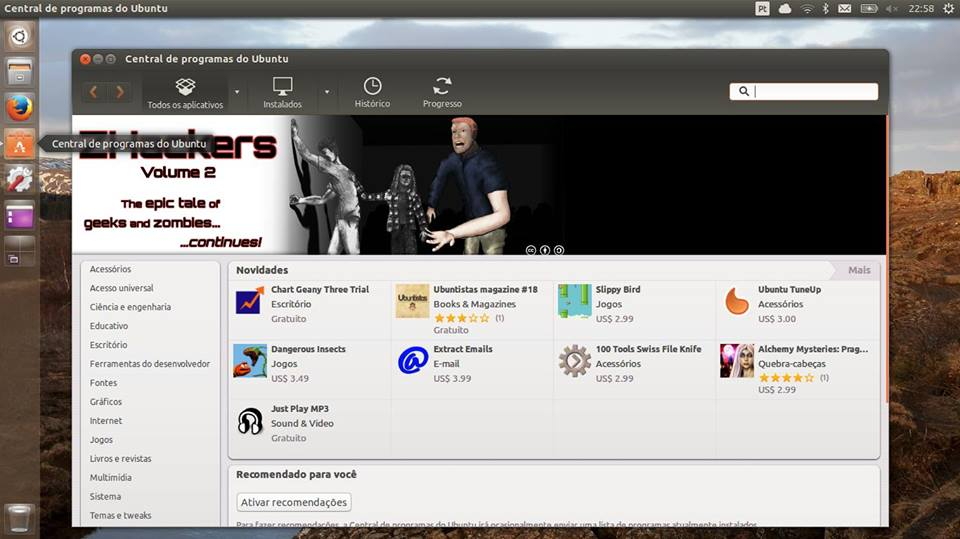
\includegraphics[scale=0.4]{linux5.png} 
\end{figure}
Resultado da procura do coq no gerenciador:\\
\begin{figure}[!htb]
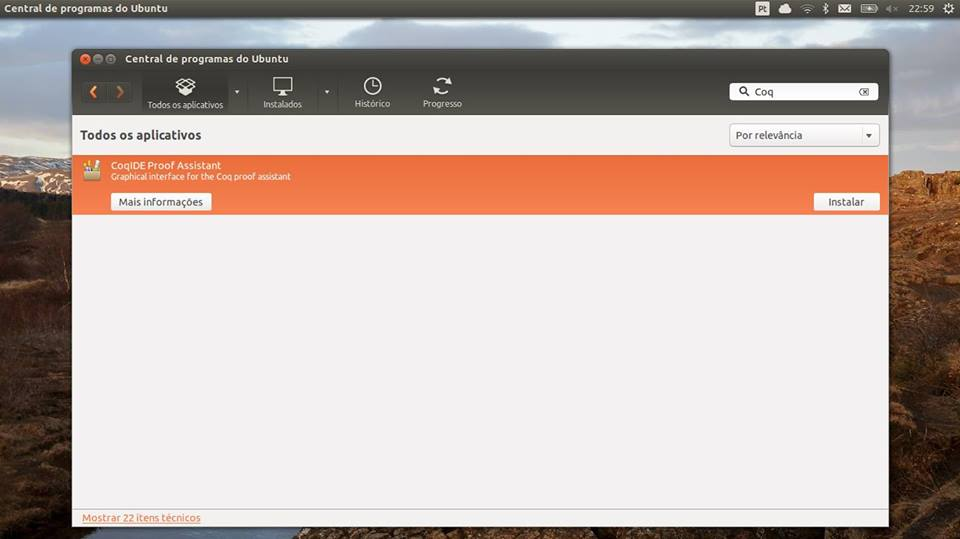
\includegraphics[scale=0.4]{linux2.png} 
\end{figure}
Informar o usu\'{a}rio mestre do linux, o q possui os privil\'{e}gios de instala\c{c}\~{a}o de programas.\\
\begin{figure}[!htb]
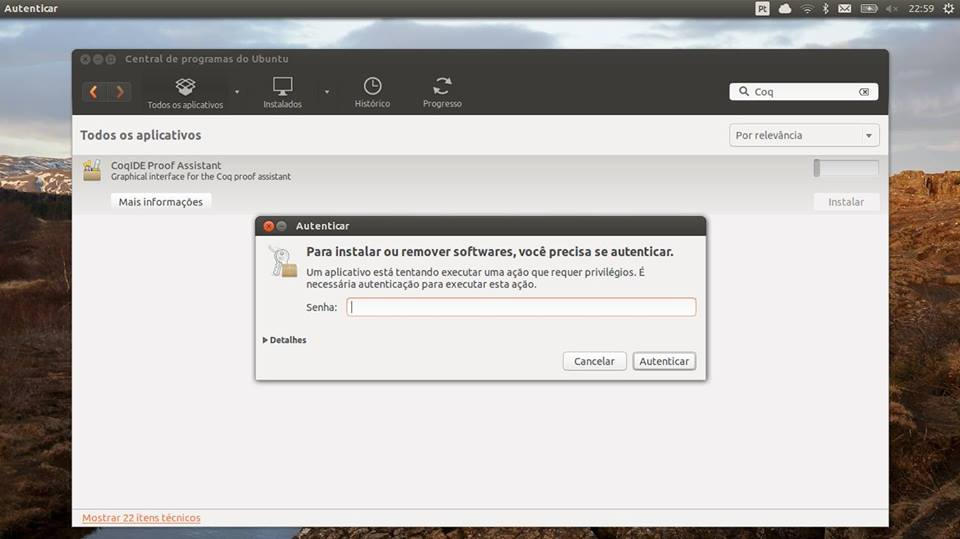
\includegraphics[scale=0.4]{linux1.png} 
\end{figure}
Indicativo que o programa foi instalado.\\
\begin{figure}[!htb]
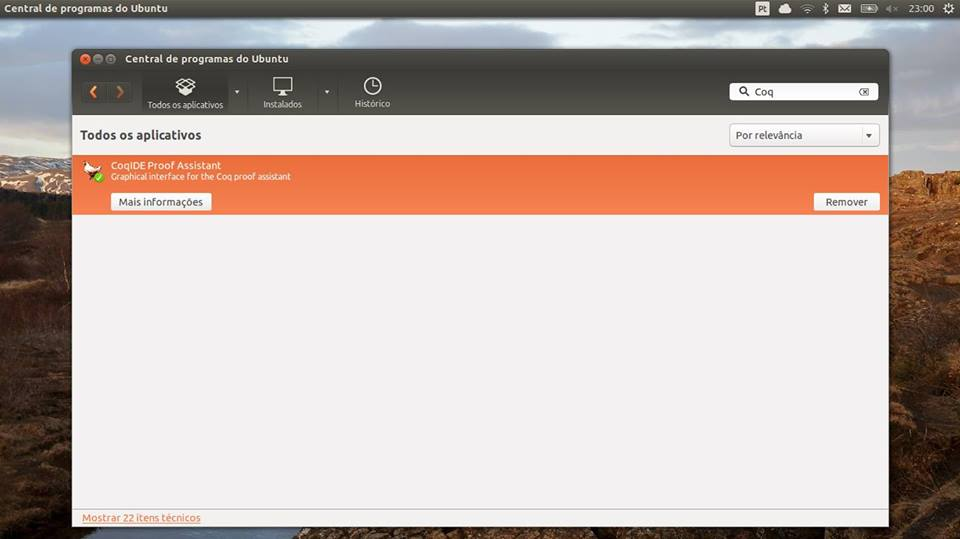
\includegraphics[scale=0.4]{linux3.png} 
\end{figure}
Depois de instalado o \'{i}cone do Coq aparece no painel.\\
\begin{figure}[!htb]
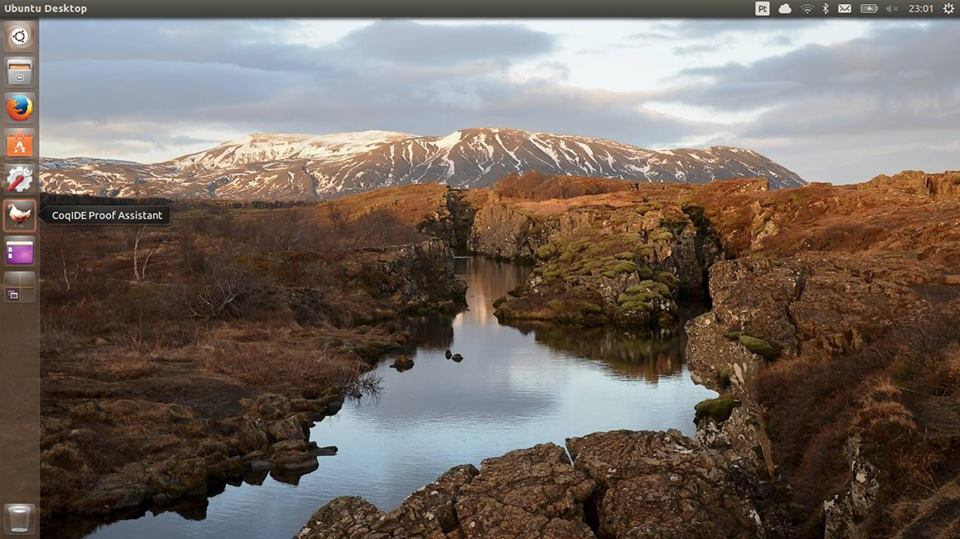
\includegraphics[scale=0.4]{linux6.png}
\end{figure}
Janela do Coq aberta:\\
\begin{figure}[!htb]
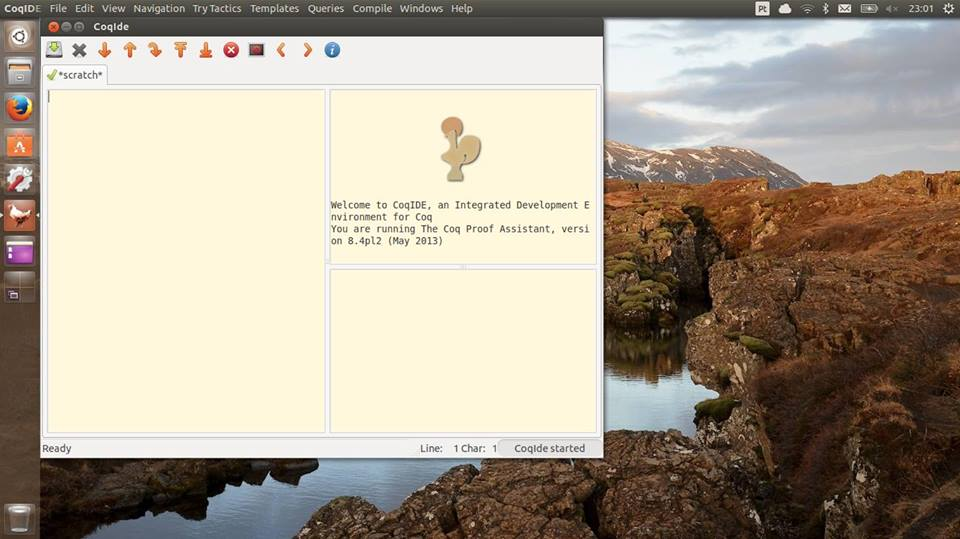
\includegraphics[scale=0.4]{linux4.png}
\end{figure}
\section{Instala\c{c}\~ao para MacOS}

\bibliographystyle{plain}
\bibliography{apostila}

\end{document}
